\documentclass[12pt,twoside]{report}


%%%%%%%%%%%%%%%%%%%%%%%%%%%%%%%%%%%%%%%%%%%%%%%%%%%%%%%%%%%%%%%%%%%%%%%%%%%%%

% Definitions for the title page
% Edit these to provide the correct information
% e.g. \newcommand{\reportauthor}{Timothy Kimber}

\newcommand{\reporttitle}{ Gaussian Processes for \\ Optimal Sensor Position \\[0.5cm] { \Large  MSc Project Report}}
\newcommand{\reportauthor}{Adrian \textsc{Löwenstein}}  %\\ \phantom{blank author} 
\newcommand{\supervisor}{Dr. Rossella \textsc{Arcucci} } % \\ Miguel \textsc{Molina-Solana}

\newcommand{\degreetype}{Computing (Machine Learning)}

%%%%%%%%%%%%%%%%%%%%%%%%%%%%%%%%%%%%%%%%%%%%%%%%%%%%%%%%%%%%%%%%%%%%%%%%%%%%%

% load some definitions and default packages
%%%%%%%%%%%%%%%%%%%%%%%%%%%%%%%%%%%%%%%%%
% University Assignment Title Page 
% LaTeX Template
% Version 1.0 (27/12/12)
%
% This template has been downloaded from:
% http://www.LaTeXTemplates.com
%
% Original author:
% WikiBooks (http://en.wikibooks.org/wiki/LaTeX/Title_Creation)
%
% License:
% CC BY-NC-SA 3.0 (http://creativecommons.org/licenses/by-nc-sa/3.0/)
% 
%
%%%%%%%%%%%%%%%%%%%%%%%%%%%%%%%%%%%%%%%%%
%----------------------------------------------------------------------------------------
%	PACKAGES AND OTHER DOCUMENT CONFIGURATIONS
%----------------------------------------------------------------------------------------
\usepackage[a4paper,hmargin=2.8cm,vmargin=2.0cm,includeheadfoot]{geometry}
\usepackage{caption}
\usepackage{subcaption}
\usepackage{textpos}
\usepackage{natbib} % for bibliography
\usepackage{tabularx,longtable,multirow}%hangcaption
\usepackage{fncylab} %formatting of labels
\usepackage{fancyhdr} % page layout
\usepackage{url} % URLs
\usepackage[english]{babel}
\usepackage{amsmath}
\usepackage{graphicx}
\usepackage{dsfont}
\usepackage{epstopdf} % automatically replace .eps with .pdf in graphics
\usepackage{backref} % needed for citations
\usepackage{array}
\usepackage{latexsym}
\usepackage[pdftex,pagebackref,hypertexnames=false,colorlinks]{hyperref} 
% provide links in pdf



\hypersetup{pdftitle={},
  pdfsubject={}, 
  pdfauthor={},
  pdfkeywords={}, 
  pdfstartview=FitH,
  pdfpagemode={UseOutlines},% None, FullScreen, UseOutlines
  bookmarksnumbered=true, bookmarksopen=true, colorlinks,
    citecolor=black,%
    filecolor=black,%
    linkcolor=black,%
    urlcolor=black}

\usepackage[all]{hypcap}


%\usepackage{color}
%\usepackage[tight,ugly]{units}
%\usepackage{float}
%\usepackage{tcolorbox}
%\usepackage[colorinlistoftodos]{todonotes}
% \usepackage{ntheorem}
% \theoremstyle{break}
% \newtheorem{lemma}{Lemma}
% \newtheorem{theorem}{Theorem}
% \newtheorem{remark}{Remark}
% \newtheorem{definition}{Definition}
% \newtheorem{proof}{Proof}


%%% Default fonts
\renewcommand*{\rmdefault}{bch}
\renewcommand*{\ttdefault}{cmtt}



%%% Default settings (page layout)
\setlength{\parindent}{0em}  % indentation of paragraph

\setlength{\headheight}{14.5pt}
\pagestyle{fancy}
\renewcommand{\chaptermark}[1]{\markboth{\chaptername\ \thechapter.\ #1}{}} 

\fancyfoot[ER,OL]{\sffamily\textbf{\thepage}}%Page no. in the left on odd pages and on right on even pages
\fancyfoot[OC,EC]{\sffamily }
\renewcommand{\headrulewidth}{0.1pt}
\renewcommand{\footrulewidth}{0.1pt}
\captionsetup{margin=10pt,font=small,labelfont=bf}


%--- chapter heading

\def\@makechapterhead#1{%
  \vspace*{10\p@}%
  {\parindent \z@ \raggedright \sffamily
    \interlinepenalty\@M
    \Huge\bfseries \thechapter \space\space #1\par\nobreak
    \vskip 30\p@
  }}

%---chapter heading for \chapter*  
\def\@makeschapterhead#1{%
  \vspace*{10\p@}%
  {\parindent \z@ \raggedright
    \sffamily
    \interlinepenalty\@M
    \Huge \bfseries  #1\par\nobreak
    \vskip 30\p@
  }}

\allowdisplaybreaks

% load some macros
% Here, you can define your own macros. Some examples are given below.

\newcommand{\R}[0]{\mathds{R}} % real numbers
\newcommand{\Z}[0]{\mathds{Z}} % integers
\newcommand{\N}[0]{\mathds{N}} % natural numbers
\newcommand{\C}[0]{\mathds{C}} % complex numbers
\renewcommand{\vec}[1]{{\boldsymbol{{#1}}}} % vector
\newcommand{\mat}[1]{{\boldsymbol{{#1}}}} % matrix
\newcommand{\norm}[1]{\left\lVert#1\right\rVert}


\date{\today}

\begin{document}

% load title page
% Last modification: 2015-08-17 (Marc Deisenroth)
\begin{titlepage}

\newcommand{\HRule}{\rule{\linewidth}{0.5mm}} % Defines a new command for the horizontal lines, change thickness here


%----------------------------------------------------------------------------------------
%	LOGO SECTION
%----------------------------------------------------------------------------------------


\includegraphics[width = 4cm]{./figures/imperial}\\[0.5cm] 

\center % Center remainder of the page

%----------------------------------------------------------------------------------------
%	HEADING SECTIONS
%----------------------------------------------------------------------------------------

\textsc{\Large Imperial College London}\\[0.5cm] 
\textsc{\large Department of Computing}\\[0.5cm] 

%----------------------------------------------------------------------------------------
%	TITLE SECTION
%----------------------------------------------------------------------------------------

\HRule \\[0.4cm]
{ \huge \bfseries \reporttitle}\\ % Title of your document
\HRule \\[1.5cm]
 
%----------------------------------------------------------------------------------------
%	AUTHOR SECTION
%----------------------------------------------------------------------------------------

\begin{minipage}{0.4\textwidth}
\begin{flushleft} \large
\emph{Author:}\\
\reportauthor % Your name
\end{flushleft}
\end{minipage}
~
\begin{minipage}{0.4\textwidth}
\begin{flushright} \large
\emph{Supervisor:} \\
\supervisor % Supervisor's Name
\end{flushright}
\end{minipage}\\[4cm]


%----------------------------------------------------------------------------------------
%	FOOTER & DATE SECTION
%----------------------------------------------------------------------------------------
\vfill % Fill the rest of the page with whitespace
Submitted in partial fulfillment of the requirements for the MSc degree in
\degreetype~of Imperial College London\\[0.5cm]

\makeatletter
\@date 
\makeatother


\end{titlepage}



% page numbering etc.
\pagenumbering{roman}
\clearpage{\pagestyle{empty}\cleardoublepage}
\setcounter{page}{1}
\pagestyle{fancy}

%%%%%%%%%%%%%%%%%%%%%%%%%%%%%%%%%%%%
%\begin{abstract}
%Your abstract.
%\end{abstract}

\cleardoublepage
%%%%%%%%%%%%%%%%%%%%%%%%%%%%%%%%%%%%
%\section*{Acknowledgments}
%Comment this out if not needed.

\clearpage{\pagestyle{empty}\cleardoublepage}

%%%%%%%%%%% TABLE OF CONTENTS 
\chapter*{Abstract}

Gaussian processes (GP) have been widely used since the 1970s in the fields of geostatistics and meteorology. Current applications are in diverse fields including sensor placement.
In this project, we propose the employment of a GP model to calculate the optimal spatial positioning of sensors to study and collect air pollution data in big cities. We will then apply the results by means of a data assimilation with the data at the optimised positions.


\chapter*{Acknowledgment}

I would like to thank \textit{Imperial College London} for the opportunity I was given to pursue my studies this prestigious university. \\

I would like to thank my supervisor Dr. Rossella Arcucci  of the \textit{Data Science Institute}, for her help and wise counselling throughout the project. \\

An finally, I would like to thank my girlfriend, and friends from Imperial College, who supported me during this project. \\



%--- table of contents
\fancyhead[RE,LO]{\sffamily {Table of Contents}}
\tableofcontents 


\clearpage{\pagestyle{empty}\cleardoublepage}
\pagenumbering{arabic}
\setcounter{page}{1}
\fancyhead[LE,RO]{\slshape \rightmark}
\fancyhead[LO,RE]{\slshape \leftmark}

\pagebreak



%%%%%%%%%%% CHAPTER: INTRODUCTION
\chapter{Introduction}



The optimisation of sensor position is a very common problem in many applications. The reliability of very complex systems often depend on the choice sensor position. The cost induced by the incorrect placement or un-necessary sensor placement could be very important. There is therefore a real need for optimal sensor placement in the industry and in research applications. \\

Main Problem \\
Optimise sensor positions. Common Problem. \\



Solution to the Problem
Investigate and Explore the solution proposed by \citet{krause_near-optimal_2008} on near-optimal optimisation \\
\\ > Details on the Process
Gaussian Processes \\


Applications : \\
Application to the Problem of Data Assimilation. Assimilate data on a limited number of points. Use the optimal sensors for the Data Assimilation and see if the results are better than random.  Can be used on other sets.  \\

Challenge is the size of of the candidate set. \\


 



\todo{Write Intoduction}


\todo{Write Problem Statement : Why we need that ? What solution ?
}



 
%%%%%%%%%%% CHAPTER: LITERATURE REVIEW
\chapter{Literature Review}


In this chapter, we will cover the literature and the theory that will be used throughout the project. First, we will review the context of the project and how it fits into the \textbf{MAGIC} project. Then our focus goes to the definition of \textbf{Gaussian Processes} (GP) and how they are used in the context of geospatial data. Furthermore, the use of GP relies heavily on \textbf{Covariance} matrixes which need to be estimated. Those tools enable us to create \textbf{optimisation} algorithms for the position of sensors. Finally, we will quickly explore the concepts of \textbf{Data Assimilation} (DA) that will be used to validate the results of the optimisation. 

\section{The MAGIC Project}

This work is done in the context of the \textbf{Managing Air for Green Inner Cities} project. This is a multidisciplinary project and has for objective to find solutions to the pollution and heating phenomenons in cities. Traditionally, urban environmental control relies on polluting and energy consuming heating, ventilation and cooling (HVAC) systems. The usage of the systems increases the heat and the pollution levels, inducing an increased need for the HVAC. The MAGIC project aims at breaking this vicious circle and has for objective to provide tools to make possible the design of cities acting as a natural HVAC system. \\


This has been extensively discussed by  \cite{song_natural_2018}.  For this purpose, integrated management and the decision-support system is under development. It includes a variety of simulations for pollutants and temperature at different scales; a set of mathematical tools to allow fast computation in the context of real-time analysis; and cost-benefit models to asses the viability of the planning options and decisions. \\

As explained by \cite{song_natural_2018}, the test site which has been selected to conduct the study is a real urban area located in London South Bank University (LSBU) in  Elephant and Castle, London. In order to investigate the effect of ventilation on the cities problem, researchers in the MAGIC project have created simulations and experiments both in outdoor and indoor conditions, on the test site. They used wind tunnel experiments and computational fluid dynamics (CFD) to simulate the outdoor environment. Further works include the development of reduced-order modelling (ROM) in order to make faster the simulations while keeping a high level of accuracy \citep{arcucci_effective_2018}. \\

Another key research direction in the use Data Assimilation (DA) and more specifically Variational DA (VarDA) for assimilating measured data in real time and allowing better prediction of the model in the near future \citep{arcucci_effective_2018}. The further use of those methods would be the optimisation of the position of the sensors which provide information for the VarDA.


\section{Gaussian Processes}\label{sec:theory:gp}

In this section, we will review Gaussian Processes (GP) which are probabilistic models for spatial predictions based on observations assumption. \\ 

As explained by \citet[p.~29]{rasmussen_gaussian_2006}, the history of Gaussian Processes goes back at least as far as the 1940s. A lot of usages were developed in various fields. Notably for predictions in spatial statistics \citep{cressie_statistics_1991}.  Applied in particular in Geostatistics with methods known as \textit{kringing}, and in Meteorology. Gradually GP started to be used in more general cases for regression. Nowadays it is often used in the context of Machine Learning. \\


For our problem, we will be modelling the data of the sensor with GPs.
%As for sensor optimisation, we will follow the approach that was developed by \citet{krause_near-optimal_2008}. This method relies on GP for finding a near-optimal solution to the problem of placing sensors. 

\todo{Mention the main assumption that the data needs to be gaussianly distributed and iid samples (Maybe already explained)}

%\subsection{Sensor Data Modelling}

\subsection{Multivariate Gaussian Distribution}

GP will serve as a basic tool in our project. In the space we are monitoring we have a certain number of sensors measuring a certain quantity, such as temperature, pressure, speed of the wind or the concentration of a pollutant at a given position. We assume that the measured quantity has a \textit{multivariate Gaussian joint distribution} between each point of the space. The associated random variable is $\X_\V$ for the set of locations $\V$ we would have the following distribution : $P(\X_\V = \vec{x}_\V) \sim \mathcal{N}(\mu_\V, K_{\V\V}) $, or explicitly : 


\begin{equation}
    P(\X_\V = \vec{x}_\V) \frac{1}{(2\pi)^{n/2} |K_{\V\V}|} \exp^{-\frac{1}{2}(\vec{x}_\V - \mu_\V)^T K_{\V\V}^{-1} (\vec{x}_\V - \mu_\V)}
\end{equation}


\subsection{Prediction with Gaussian Processes}
Let us still consider that we have the set of locations $\V$ and a set of sensors $\A$. In order to predict the quantity at positions were we have no sensors ($\V \backslash \A $) we can use a Gaussian Process. This allows us to infer a function belonging the the function space : $\mathcal{GP}(\mathcal{M}(\vec{x}), \mathcal{K}(\vec{x},\vec{x}'))$.  This GP is associated with a \textbf{mean function} $\mathcal{M}(\cdot)$ and a symmetric positive-definite \textbf{kernel function} $\mathcal{K}(\cdot,\cdot)$. We will denote the mean function values for a set of positions $\A$ by $\mu_\A$ and the kernel function values, or covariance matrix, between those points by $K_\A$. More detailed definitions are available in \citet[p.~13-16]{rasmussen_gaussian_2006}. \\

For a set of observations $\vec{x}_\A$ at positions $\A$ we can express for a finite set of other positions $\V \backslash \A $ the conditional distribution of those values. This means that we are able, for each point $y \in \V \backslash \A $, to predict the mean and the variance of $\vec{x}_y$. Using conditional distribution for the Multivariate Gaussian Distribution \citep[p.~193]{deisenroth_mathematics_2018}, we are able to express the following : 
\begin{align}
    P(\X_y | \vec{x}_\A ) &= \mathcal{N}(\mu_{y | \A}, K_{y | \A}) \\
    \mu_{y | \A} &= \mu_y + K_{y\A} K_{\A\A}^{-1} (y - \mu_y)\\ 
    K_{y | \A} &=  K_{yy} - K_{y\A} K_{\A\A}^{-1} K_{\A y} \label{equ:covGP}
\end{align}

An important point to notice is that the predicted covariance for the point y is not dependent of the values measured at $\A$, this is really useful because it allows us to define the uncertainty at $y$ without using only the covariance. \\

\subsection{Scalable Gaussian Processes} 

The biggest weakness of Standard GPs is their complexity. For $p$ training points, the algorithm requires the inversion of a $p \times p$ covariance matrix $K_{pp}$. \citet{liu_when_2018} gives an extensive review of all methods used to make the GPs more scalable. Those methods are evaluated with regards to their \textit{scalability} and their \textit{capability}. \\ 

We redefine notations used here to explore scalable Gaussian Processes.  We consider $n$ training points $\mathbf{X}= \{\vec{x}_i \in \mathbb{R}^d \}^n_{i=1}$, and observations $\vec{y} = \{y_i = y(\vec{x}_i) \in \mathbb{R} \}^n_{i=1} $. GP aims at inferring the function $f : \mathbb{R}^d \mapsto \mathbb{R}$ that describes the best the training data. This function belongs to the  function space $\mathcal{GP}(\mathcal{M}(\vec{x}), \mathcal{K}(\vec{x},\vec{x}'))$. We then replace the conditionals .  In order to obtain the observations we formally add gaussian noise $\mathcal{N}(0,\epsilon_nI_n)$ to the inferred function values (we didn't need that in the previous section). 


% The aim of global approximation is to reduce the size of the covariance matrix, in order to make the computation scalable. There are several ways to proceed: \textbf{subset of data} method where we reduce the size of the training set; the \textbf{sparse kernel} methods where we exploit a low-rank representation of the GP (\textbf{sparse approximation}). \\ 
 
 \paragraph{Subset of Data}



The \textbf{subset of data method} (SoD) is a very simple strategy that only requires to create a subset of the original training data. The resulting cost of the GP is only of $\mathcal{O}(m^3)$ with $m$ the number of points in the subset and $m << p$.  \\

 \paragraph{Sparse Kernel}
 
The \textbf{sparse kernel} approach is the idea to reduce the importance of the points far from each other and imposing sparsity of the covariance by setting to zero the elements of the matrix $K_{pp}$ that are below a certain threshold. The resulting complexity being of $\mathcal{O}(\alpha p^3)$ with $0 < \alpha < 1$. The difficulty here is to ensure the positive definiteness of the resulting covariance. \\

 \paragraph{Low Rank Approximation}
 
 In \citet{foster_stable_2009}, the idea of using the Truncated Singular Values Decomposition (TSVD) as a method of obtaining a low-rank, well conditioned version of the covariance matrix was developed. The inconvenient of this method is that the TSVD is an operation of complexity $\mathcal{O}(n^3)$. We will propose in the following chapter a solution inspired by idea. 

\paragraph{Sparse Approximations}

The \textbf{sparse approximation} methods are very diverse and are allowed by different kinds of approximations : the \textbf{approximation of the prior} ; the \textbf{approximation of the posterior} ; \textbf{structured sparse approximations}. \\

\textbf{Prior approximation} modifies the joint prior $p(\mathit{f,f_*})$ between the training data $\mathit{f}_*$ and the test data $\mathit{f}$ by assuming independence between them knowing \textbf{inducing variables} $\mathit{f}_m$ : $\mathit{f}_* \perp \mathit{f} \; | \; \mathit{f}_m$. We also define the Nyström notation for the covariance : $\vec{Q}_{ab} = \vec{K}_{am} \vec{K}_{mm}^{-1} \vec{K}_{mb} $. We are then able to express the conditional probabilities for $p(\mathit{f} | \mathit{f}_m) = \mathcal{N}(\mathit{f} \; | \; \vec{K}_{nm}\vec{K}_{mm}^{-1}\mathit{f}_m \, , \vec{K}_{nn} - \vec{Q}_{nn})$ and  $p(\mathit{f}_* | \mathit{f}_m)  = \mathcal{N}(\mathit{f} \; | \; \vec{K}_{*m}\vec{K}_{mm}^{-1}\mathit{f}_* \, , \vec{K}_{**} - \vec{Q}_{**})$  and approximate them to : $q(\mathit{f} | \mathit{f}_m)$ and  $q(\mathit{f}_* | \mathit{f}_m)$ by replacing respectively the covariances by   $\tilde{\vec{Q}}_{nn}$ and $\tilde{\vec{Q}}_{**}$. This approximation allows for a computation with a reduced complexity of $\mathcal{O}(mn^2)$. \\

 In order to select an appropriate approximate covariance $\tilde{\vec{Q}}_{nn}$ and $\tilde{\vec{Q}}_{**}$, different methods are referenced such as  SoR, DTC, FITC and PITC.
 
 
 \textit{Subset of Regressor} (SoR) fixes both covariances to $0$, forcing a deterministic view. 
 
 In the \textit{Deterministic Training Conditional} (DTC), imposes a deterministic training $\tilde{\vec{Q}}_{nn} = 0$ but keeps the exact test conditional $p(\mathit{f}_* | \mathit{f}_m)$. 
 
 Another approach is the \textit{Fully Independent Training Conditional} (FITC). Here we keep exact the test conditional but we approximate the training by considering that each realisation is independent from each other : the $\{\mathit{f}_i\}^n_{i=1}$ are fully independent, and we take the covariance to be $\tilde{\vec{Q}}_{nn} = diag(\vec{K}_{nn} - \vec{Q}_{nn} ) $. This leads to better results than the two previous methods. 
 In order to further improve this method the idea of \textit{Partially Independent Training Conditional} (PITC) was introduced. Here we consider that not all the training points are independent, but only some of them. This leads to an independence by blocks, and an block-diagonal covariance approximation : $\tilde{\vec{Q}}_{nn} = blkdiag(\vec{K}_{nn} - \vec{Q}_{nn} ) $. 
 
In those methods, the choice of the $m$ \textit{inducing points} is crucial to enable a good approximation. \\


Another way to see the problem is to \textbf{approximate the posterior} $p(\mathit{f,f_*} | \vec{y})$ of the GP instead of the prior $p(\mathit{f,f_*})$, by replacing it with a variational distribution  $q(\mathit{f,f_*} | \vec{y})$. The main method is called the \textit{Variational Free Energy} (VFE), and has been developed by \cite{titsias_variational_2009}. We optimise the variational parameters and hyperparameters of the  approximation by minimising the KL divergence between the two distributions : 


\begin{align}
    KL(q(\mathit{f,f_*} | \vec{y})\; || \;  p(\mathit{f,f_*} | \vec{y})) &= \log p(\vec{y}) - \left\langle  \log \frac{p(\mathit{f,f_*},\vec{y})}{q(\mathit{f,f_*} | \vec{y})}\right\rangle_{q(\mathit{f,f_*} | \vec{y})} \\
    &= \log p(\vec{y}) - F_q
    \label{equ:vfe_kl}
    \end{align}  
    
As the KL divergence is positive, minimising this quantity is equivalent to maximising the Variational Free Energy (VFE): $F_q$ (also called Evidence Lower Bound - ELBO). A tighter bound can be derived to replace $F_q$ : 
\begin{equation}
    F_{VFE} = \log q_{DTC}(\vec{y}) - \frac{1}{2\sigma_\epsilon^2} tr(\vec{K}_{nn} - \vec{Q}_{nn})
\end{equation}

In the DTC we maximised the likelihood $q_{DTC}(\vec{y})$ and here we add only an additional term. This has 3 functions: it acts as a regulariser against over-fitting; it helps finding a good inducing set; it always improves the ELBO with increasing $m$.  \\

Finally, the last global approach is the \textit{structured sparse approximations}. The main idea is to speed up the computation of the inversion of the covariance matrix and multiplication by a vector: $\vec{K}_{nn}^{-1}\vec{y}$. For that fast \textit{matrix vector multiplication} (MVM) is used, it solves the linear system by using conjugate gradients. Several improvements have been proposed, especially when the covariance matrix $\vec{K}_{nn}$ has some algebraic structure, such as in the \textit{Kroenecker Methods} and the \textit{Toeplitz Methods}. Those methods require also inputs having a grid structure, therefore not directly applicable in our project.  In order to generalise those methods to any kind of data structure, the method of structured kernel interpolation (SKI) was also proposed by \citet{wilson_kernel_2015}. Inducing points are created using local linear interpolation techniques and constrained to the grid structure. This method has drawbacks such as exponential growth of inducing points in high dimension; discontinuous predictions and overconfident variance. 


\paragraph{Remarks on the Approximation Methods}
Many of those methods require a lot of computing to come up with the GP approximation. Some of them require to find the best inducing points representing the observations of the original GP. Once this step is done, they allow a very computationaly efficient prediction. Unfortunately we will see that the nature of the optimisation problem proposed by \citet{krause_near-optimal_2008}, makes it impossible for us to use most of those algorithms. Indeed we will see that our observation set is constantly changing with the iterations of the algorithm, forcing us to compute for each iteration a new set of inducing points. This creates a new bottleneck. 
%
%\subsubsection{Local Approaches}
%
%Applying the principle de Divide and Conquer (D\&C), the main idea is to use \textit{local experts} to create a full GP representation. It has the main advantage to enable naturally \textit{parallelisation} and to capture \textit{non-stationary} features. We can use naive local experts (NLE), or more complex combinations of localised experts such as mixture of experts (MoE) or Products of Experts (PoE). \\
%
%In naive local experts (NLE), each expert is trained on a different subset of the space. For a training set of points $\mathcal{D}$ and its subsets $\mathcal{D}_i$, we have the prediction of the expert $\mathcal{M}_i$ inside a subregion $\Omega_i$ : $\vec{x}_* \in \Omega_i$ such as $p(y_* | \mathcal{D}, \vec{x}_*) \approx p_i(y_* | \mathcal{D}_i, \vec{x}_*) $. In \textit{inductive} NLE, the space is first partitioned and each expert is trained before choosing the appropriate one of the prediction. The partition is therefore fixed beforehand. In \textit{transductive} NLE, once the prediction point $\vec{x}_*$ has been chosen,  the expert $\mathcal{M}_*$ is trained locally on a subset $\mathcal{D}_*$ close to $\vec{x}_*$. A few drawbacks are the discontinuities at the boundaries between the subregions and the fact that it generalises badly to all the regions. \\


\section{Covariance Matrix} \label{sec:cov_est}

We have seen how GPs are defined and can be made more scalable. In order to have good results, we need to have a good estimate of the covariance matrix between the points of our mesh. \\



%Many application requires the covariance to be estimated because of the lack of measures. Very often a limited number of sensors has been in position and the key challenge is to interpolate the covariance. talk of the different methods\\

In our specific case, we already have at our disposal a very dense network of measurement. With more than $100'000$ different locations we don't need to explore the space outside of those points. Unfortunately, the sample covariance is a very bad estimator of the true covariance in high dimensional settings such as ours \citep{pourahmadi_covariance_2011}. \\


We will see the properties that our covariance must have to accurately represent our data, before discussing the best ways of estimating the covariance matrix.


\subsection{Properties of Covariance}

By definition a covariance matrix must be \textbf{positive-definite} and \textbf{symmetrical} \citep[p.~80]{rasmussen_gaussian_2006}. \\

A covariance function between two inputs $x$ and $x'$ is \textbf{stationary}   when it is invariant to translation. Thus, when it is a function of $x' - x$. \\
In a covariance function that is \textbf{isotropic}, we remove the dependence of the direction and, it becomes a function of the distance between the two points: $|x' - x|$. The isotropy of the covariance function is a stronger assumption than  \\ 

In our problem, we can't assume that the process is stationary nor isotropic. Our space is 3-dimensional and not homogeneous. The presence of the buildings and other obstacles that likely to make environment variables less smooth \citep{paciorek_nonstationary_2004}. Also, it has been shown by \citet{krause_near-optimal_2008} that non-stationary covariance matrixes give better results than stationary or isotropic. This makes us choose a non-stationary covariance matrix for the  GPs of our problem.


\subsection{Covariance Estimation}


There are several ways to estimate the covariance matrix of a random process. In this part we are going to expose some simple, yet computationally efficient ways to estimate the true covariance matrix $\vec{\Sigma}$ of a gaussian distributed dataset.\\

We consider the process $Y$ in $p$ different locations at $n$ sampling times. $\vec{Y}_i = (Y_{1i}, \dots, Y_{pi})$, with $i = 1 \dots n$, and $X$ the cantered process. \\

\subsubsection{Sample Covariance}

The simplest estimator of the covariance matrix is the \textbf{sample covariance matrix} $ \vec{\hat{S}} $ directly computed from the captured data. It's size if of $p\times p$. This estimator is an unbiased estimator of the true covariance matrix $\vec{\Sigma}$. It is also the expression of the \textbf{maximal likelihood} estimator. 

\begin{align}
    \vec{\hat{S}} &= \frac{1}{n} \sum_{i=1}^n (\vec{Y}_i - \bar{\vec{Y}})\cdot (\vec{Y}_i - \bar{\vec{Y}})^T, \quad \bar{\vec{Y}} = \frac{1}{T} \sum_{i=1}^n \vec{Y}_i \\
    \vec{\hat{S}} &= \frac{1}{n} \sum_{i=1}^n \vec{X}_i \cdot \vec{X}_i^T 
\end{align}

Unfortunately, this covariance is often singular when $p >> T$ \citep{fan_overview_2015}, and its estimation error is very important \citep{ledoit_honey_2003}.

\subsubsection{Shrinkage Method}


%
%\paragraph{Estimating a Spatial Covariance} 
%
%\cite{nott_estimation_2002-1} proposed to fit local variograms in order to approaximate the covariance matrix. It is a method that was developped in \cite{cressie_statistics_1991}. \\
%
%Another method is the use of spatial deformation of the kernel in order to obtain non-stationarity \citep{sampson_nonparametric_1992}. \\
%
%Several different approaches are developed in the literature, notably the works of \citep{fan_overview_2015} and \cite{guttorp_20_1994} which is more focused on spatial data. 
%
%\textbf{Note :} This section needs further developments, in order to find an implement the best possible approach in \textit{coordination} with the scalable Gaussian Processes. 
%

A good alternative to the sample covariance matrix is the shrinkage method developed by \citet{ledoit_improved_2003}. It was originally proposed for the the purpose of improving the mean-variance portfolio optimisation in finance. \\

Intuitively, the algorithm tends to pull most extreme coefficients of the covariance matrix towards more central values, thus shifting every eigenvalue according to a given offset. The principle of shrinkage estimator is to make a compromise between two extreme estimators : One that is structured, that we call the shrinkage target $\vec{F}$, and one that is unstructured, the sample covariance matrix  $\vec{S}$. To make this compromise we take a  convex linear combination of the two estimators and optimise the shrinkage constants. The shrinkage target $F$ is often defined as proportional to the identity matrix \citet{chen_shrinkage_2010} : 

\begin{equation}
	\vec{\hat{F}} = \frac{\text{Tr}(\vec{\hat{S}})}{p} \vec{I}
\end{equation}

The shrinkage oracle estimator is defined such as :

\begin{equation}
	\vec{\hat{\Sigma}} = \rho\vec{\hat{S}} + (1- \rho )\vec{\hat{S}}
	\label{equ:oracle}
\end{equation}

The optimisation problem was expressed as follows by \citet{ledoit_well-conditioned_2004}, ($\lVert  \cdot \rVert_F$ being the Frobenius matrix norm ) :

\begin{align}
	\min_\rho \quad & \mathbb{E}\left\{ \, \lVert \vec{\hat{\Sigma}} - \vec{\Sigma} \rVert_F^2 \, \right\} \\
	\text{s.t.} \quad &  \vec{\hat{\Sigma}} = \rho\vec{\hat{S}} + (1- \rho )\vec{\hat{S}} \\
\end{align}

Which has for solution : 

\begin{equation}
	\rho_O = \frac{\mathbb{E}\left\{\text{Tr}[(\vec{\Sigma} -\vec{\hat{S}} ) (\hat{\vec{F}} -\vec{\hat{S}} )]\right\}}{\mathbb{E}\left\{ \, \left\lVert \vec{\hat{S}} -\vec{\hat{S}} \right\rVert_F^2 \, \right\}}
\end{equation}


This solution is dependant of the true covariance matrix $\vec{\Sigma}$ and therefore can't be directly implemented. \citet{ledoit_well-conditioned_2004} propose then a method that is to \textit{asymptotically} approximate the estimator. 

\begin{equation}
	\hat{\rho}_{LW}^* =  \frac{\sum_{i=1}^n \left\lVert \vec{Y_i}\vec{Y_i}^T - \vec{\hat{S}} \right\rVert_F^2   }{n^2 \left[ \text{Tr}( \vec{\hat{S}} ^2) - \frac{ \text{Tr}^2( \vec{\hat{S}} ) }{p} \right]}
\end{equation}

They proved that for $n,\, p \rightarrow \infty $ and $p/n \rightarrow c $ with $0<c < \infty $, this quantity converges to the optimal solution.  By including it in the equation \ref{equ:oracle} we obtain the Ledoit-Wolf (LW) covariance estimator.



\subsubsection{Oracle Approximating Shrinkage (OAS)}

An alternative proposed by \citet{chen_shrinkage_2010}, is called the Oracle Approximating Shrinkage. It builds itself on the LW estimator, but with a  smaller Mean Squared Error than the LW estimator. \\

By defining an iterative method to estimate he shrinkage constant, and by using the gaussian assumption, they have been able to develop a closed form expression for the shrinkage constant $0 < \rho^*_{OAS}  \leq 1$ : \\

\begin{equation}
	\rho^*_{OAS} = \min \left(   \frac{\left(\frac{1-2}{p}\right) \text{Tr}( \vec{\hat{S}} ^2) -  \text{Tr}^2( \vec{\hat{S}} ) }{\left( \frac{n+1-2}{p}\right)\left[ \text{Tr}( \vec{\hat{S}} ^2) - \frac{ \text{Tr}^2( \vec{\hat{S}} ) }{p} \right] } \quad , \; 1\right)
	\label{equ:cov:shrink:oas}
\end{equation}

Additionally, it is shown that in cases where $p$ in much larger that $n$, the OAS estimator performs better that the LW estimator. 



\subsection{Kernel Functions}


One other alternative for estimating a covariance matrix it the choice of an arbitrary kernel function such as it is often the case in classical GP regressions. The kernel functions are often parametric and can therefore be adapted to the data, and optimised using the the Maximal Likelihood of the GP regression.  \\ 

Here, we display some classical kernel functions which are isotropic and have for parameter the lengthscale $l$. We present the squared \textbf{exponential kernel} and the \textbf{Matèrn 3/2} and \textbf{5/2} taken from \cite{rasmussen_gaussian_2006}. \\


\begin{equation}
	 K_{SE}(d) = \exp \Big(-\frac{|d|^2}{2\ell^2} \Big)
\end{equation}

\begin{equation}
	K_{3/2}(d) = \sigma^2\left(1+\frac{\sqrt{3}d}{\rho}\right)\exp\left(-\frac{\sqrt{3}d}{\rho}\right)
\end{equation} 
 
\begin{equation}
	K_{5/2}(d) = \sigma^2\left(1+\frac{\sqrt{5}d}{\rho}+\frac{5d^2}{3\rho^2}\right)\exp\left(-\frac{\sqrt{5}d}{\rho}\right)
\end{equation}

As we have data for every point we wish to predict, it is better to use some data driven technique rather than using some of those arbitrary covariance functions. Furthermore the true covariance of the space is likely to be non-stationary as \citet{krause_near-optimal_2008} explains. 


\section{Sensor Position Optimisation}\label{sec:theory:opt}

Now that we have modelled the relationship between the positions using GPS we can establish an algorithm that was developed by \citet{krause_near-optimal_2008}. The process of placing sensors in an optimal way is called in spatial statistics, \textit{sampling} or \textit{experimental design}. We want to find the optimal way to place a number of $k$ sensors (indexed by $\A$) inside the set of possible sensor locations $\S$ . So that we have $\A \subseteq \S \subseteq \V$. \\


For the rest of this section, we assume that we have at our disposal a good estimate of the covariance matrix between each point. In practice this is not that obvious as we have seen in section \ref{sec:cov_est}. The following is valid for any covariance matrix that is symmetric and positive-definite. \\ 

First, we will define how to characterise a good design in term of sensor placement. Then we will define the main optimisation algorithm and its improvements. \\ 

\subsection{Placement Criterion}

\subsubsection{Entropy Criterion}

Intuitively a good way of measuring uncertainty is the \textit{entropy}. By observing the conditional entropy of the location where no sensor was placed $\VA$, we can estimate the uncertainty remaining for those locations. We define the following conditional entropy of the un-instrumented location knowing the instrumented ones \citep[p.~16]{cover_elements_1991} :

\begin{align}
    H(\X_{\VA} | \X_\A) &= \mathbb{E}_{p(\vec{x}_{\VA},\vec{x}_\A)} \log p(\X_{\VA} | \X_\A) \\
    H(\X_{\VA} | \X_\A) &= - \sum_{\vec{x}_{\VA} \in \X_{\VA}}\sum_{\vec{x}_{\A} \in \X_{\A}} p(\vec{x}_{\VA},\vec{x}_\A) \log p(\vec{x}_{\VA}|\vec{x}_\A) \\
    H(\X_{\VA} | \X_\A) &= - \int p(\vec{x}_{\VA},\vec{x}_\A) \log p(\vec{x}_{\VA}|\vec{x}_\A) \: d\vec{x}_{\VA} \, d\vec{x}_\A 
\end{align}

For the specific case of the \textit{Multivariate Gaussian Distribution}, \citet{krause_near-optimal_2008} gives us the expression of the entropy of a point $y \in \VA$ conditioned by the set $\A$ in a closed form depending exclusively on the covariance between those elements: $K_{y | \A}$. Thus we have :  

\begin{equation}
    H(\X_{y} | \X_\A) = \frac{1}{2} \log K_{y | \A} + \frac{1}{2} \left(1 + \log 2\pi  \right) \label{equ:entGP}
\end{equation}

This formulation is extremely useful because we can directly use the expression of the covariance given by the \textit{Gaussian Process} expressed previously (\ref{equ:covGP}). \\


This conditional entropy can also be expressed using the \textit{chain rule}  \citep[p.~16]{cover_elements_1991} : 

\begin{align}
    H(\X_{\VA} | \X_\A) &= H(\X_{\VA} ,  \X_\A) -  H(\X_{\A}) \\
    &= H(\X_{\V}) -  H(\X_{\A}) 
\label{equ:chainentropy}
\end{align}

The optimal set of sensors $\A^*$ with size $|\A^*| = k$, is then defined for the minimum of this entropy. If we minimise this quantity we will reduce the uncertainty on the un-instrumented locations $\VA$ : 

\begin{align}
    \A^* &= {\arg\min}_{\A \subseteq \V : |\A| = k } \: H(\X_{\VA} | \X_\A) \\
     &= {\arg\min}_{\A \subseteq \V : |\A| = k }\:  H(\X_\V) -  H(\X_{\A}) \\
     &= {\arg\max}_{\A \subseteq \V : |\A| = k }\:  H(\X_{\A}) 
\end{align}


\subsubsection{Mutual Information Criterion}

The Entropy criterion provides an intuitive way to solve the problem, unfortunately, during experiments referenced by \citet{krause_near-optimal_2008}, it was noted that this criterion has a tendency to induce placement at the border of the space, and therefore wastes a lot of precious information. This is due to the fact that the entropy criterion is \textit{indirect} because it measures the uncertainty of the selected sensor position, instead of measuring the uncertainty of every other location of the space (which are the ones we are interested in). \\

An other criterion was proposed by \citet{caselton_optimal_1984} : the \textit{Mutual Information} (MI) Criterion. We try to maximise the mutual information between the set of selected sensors $\A$ and the rest of the space $\VA$. Using the definitions of MI provided by \citet[p.~19]{cover_elements_1991} : 

\begin{align}
    \A^* &= {\arg\max}_{\A \subseteq \V : |\A| = k } \: I(\X_{\VA} , \X_\A) \\
    &= {\arg\max}_{\A \subseteq \V : |\A| = k } \: H(\X_{\VA}) -  H(\X_{\VA} | \X_{\A})
\end{align}


Experimentally, \citet{krause_near-optimal_2008} explain that  the mutual information outperforms entropy placement optimisation. They also argue that this criterion relies heavily on the quality of the model $P(\X_\V)$ (i.e. how the covariance is modelled, see section \ref{sec:cov_est}) for giving good results. 

\subsection{Approximation Algorithm}
 
 As stated by \citet{krause_near-optimal_2008}, the problem is a \textit{NP-complete problem}. Therefore we present here an algorithm that is able to approximate in polynomial time the optimal solution, with a constant factor guarantee. \\
 
 Let us define the initial sensor set $\A_0 = \emptyset$. At each iteration we have a new sensor set : $\A$,  and for a point $y$, we define : $\bar{\A} = \V \backslash ( \A \cup y )$. We also have the set of positions that can be selected as sensors : $\S$,  and the associated set : $\U = \V \backslash \S $. \\
 
 
 The idea is to greedily add sensors until we reach the wanted number ($k$).   This greedy approach is enabled by the use of the \textit{chain rule} of entropy.  Starting from $\A = \A_0$, at each iteration we add to $\A$ the point $y \in \S \backslash A $ which decreases the least the current MI : 
\begin{align}
    y* &= {\arg \max}_{y \in \S \backslash A } \: MI(\A \cup y, \bar{\A} ) - MI(\A, \VA) \\
    &= {\arg \max}_{y \in \S \backslash A } \: H(y | \A ) - H(y | \bar{\A} )
\end{align}

In our specific case with the Multivariate Gaussian Distribution, we can take the formulation presented in equation \ref{equ:entGP} and rewrite the objective to : 

\begin{align}
    y*  &= {\arg \max}_{y \in \S \backslash A } \: \frac{1}{2} \log K_{y | \A} - \frac{1}{2} \log K_{y | \bar{\A}} \\
    &= {\arg \max}_{y \in \S \backslash A } \: \log \left(\frac{K_{y | \A}}{K_{y | \bar{\A}}} \right) \\
    &= {\arg \max}_{y \in \S \backslash A } \: \frac{K_{y | \A}}{K_{y | \bar{\A}}}
\end{align}

Here we can use the GP that we have defined earlier in equation \ref{equ:covGP} to finally write the problem to solve at each iteration of the algorithm : 

\begin{equation}
    y*  = {\arg \max}_{y \in \S \backslash A } \: \frac{K_{yy} - K_{y\A} K_{\A\A}^{-1} K_{\A y} }{K_{yy} - K_{y\bar{\A}} K_{\bar{\A}\bar{\A}}^{-1} K_{\bar{\A} y} } \label{equ:updateGreedy}
\end{equation}

Then we update the set of sensors such that $\A = \A \cup y^*$, and then restart the process until $|\A| = k$. It is described in algorithm \ref{alg:greedy}  \\

\begin{algorithm}[h!]
 \KwData{Covariance matrix $K_{\V\V}$ , $k$, $\V$}
 \KwResult{Sensor Selection $\A$}
 begin\;
 \For{$j \leftarrow 1$ \KwTo $k$}{
     \For{$y \in \S \backslash \A $}{
     $\delta_y \leftarrow \frac{K_{yy} - K_{y\A} K_{\A\A}^{-1} K_{\A y} }{K_{yy} - K_{y\bar{\A}} K_{\bar{\A}\bar{\A}}^{-1} K_{\bar{\A} y} }$
     }
    $y^* \leftarrow {\arg \max}_{y \in \S \backslash A } \delta_y$ \\
    $\A \leftarrow \A \cup y^* $
 }
 \caption{Greedy/Naive Algorithm}
 \label{alg:greedy}
\end{algorithm}


This algorithm computes a solution that is very close to the optimal one if the discretisation of the space is small enough. The bound of the solution obtained is approximately 63\% of the optimal solution. If the true optimal set is $\A^*$ and $\hat{\A}$ is the solution returned by the greedy algorithm, then \citet{krause_near-optimal_2008} proves, for a small $\epsilon >0 $, that : 
 \begin{equation}
    MI(\hat{\A}) \geq (1 - \frac{1}{e}) \cdot MI(\A^*) - k\epsilon
\end{equation}

To prove that they use the notion of \textit{submodularity} \citep{nemhauser_analysis_1978} applied to the $MI(\cdot)$ function. Intuitively this represents the notion of \textit{diminishing returns} :  adding a sensor to a small set of sensors has more benefits than adding a sensor to a large set of sensors. 


\subsection{Improvements over the Algorithm}


%\subsubsection{Scaling-up}

We have exposed the main greedy algorithm to solve that optimisation problem. \citet{krause_near-optimal_2008} explains that complexity is a big issue for scaling this algorithm up. If we consider that the number of locations in our space is $|\V| = n$, and that the number of sensors to place is $k$, the complexity of the main algorithm is $\mathcal{O}(kn^4)$. They propose two solutions to this issue: a \textit{lazy procedure} that cuts the complexity to  $\mathcal{O}(kn^3)$ and a \textit{local kernel} strategy that reduces it to $\mathcal{O}(kn)$

\subsubsection{Lazy Procedure} This procedure uses strategically the notion of \textit{submodularity} and \textit{priority queues}. We can describe it intuitively: When a sensor is selected $y^*$, the other nearby points will have de decreased $\delta_y$ and will, therefore, be less desirable. Therefore if we maintain a priority queue with the ordered values of $\delta_y$ at each step we will take the top values and update them to the current value successively. If the current value needs to be updated and the location is close to the previous optimum, it would have a small $\delta_y$ and be send back in the queue. If we meet a point which has been updated and is still a the top of the queue, it means that this point is our new optimum. This technique can be efficiently applied using \textbf{binary heaps}. This algorithm is described in the algorithm \ref{alg:lazy}. \\ 


\begin{algorithm}[h]
 \KwData{Covariance matrix $K_{\V\V}$ , $k$, $\V$}
 \KwResult{Sensor Selection $\A$}
 initialisation\;
 $\A = \emptyset$ \\
 \lForEach{$y \in \S $}{$\delta_y \leftarrow + \infty$} 
 begin\;
 \For{$j \leftarrow 1$ \KwTo $k$}{
      \lForEach{$y \in \S \backslash \A $}{$current_y \leftarrow $ False }
     \While{True}{
     $y^* \leftarrow {\arg \max}_{y \in \S \backslash A } \delta_y$ \\
    \lIf{$current_{y^*}$}{break}
     $\delta_{y^*} $ is updated with \ref{equ:updateGreedy} \\
     $current_y \leftarrow $ True
     
     }
    $\A \leftarrow \A \cup y^* $
 }
\caption{Lazy Algorithm}
\label{alg:lazy}
\end{algorithm}

\subsubsection{Local Kernels} This procedure takes advantage of the structure of the covariance matrix. For many GPs, correlation decreases exponentially with the distance between points. So, the idea here is to truncate the covariance matrix to points that are the most correlated. This method is equivalent of using sparse kernels for the estimating the covariance matrix. \\ 

If we want to compute the covariance between a point of interest $y$ and a set of points $\mathcal{B} \subset \V $ we have the original covariance matrix $K_{y\mathcal{B}}$. When we remove from the set $\mathcal{B}$, the set of elements  $x \in \S$ such that $|\K(y,x)| > \epsilon $ we define the new set  $\tilde{\mathcal{B}}_y = N(y,\epsilon)$. \\

This set is defined such as it contains less than $d$ locations : $|N(y,\epsilon)| \leq d $. The truncated covariance associated with this set is named : $\tilde{K}_{y\mathcal{B}}$. Finally, we define the approximate conditional entropy $\tilde{H}_\epsilon(y | \X) \simeq H(y | \X)$, computed with truncated covariance of the points of $N(y,\epsilon)$. The $\delta_y$ values are initialised by taking the difference between the true entropy and the truncated covariance, as :
\begin{align}
    \delta_y &= \tilde{H}_\epsilon(y | \A) - \tilde{H}_\epsilon(y | \bar{\A}) \\
            &= H(y) - \tilde{H}_\epsilon(y | \V \backslash y )
\end{align}
Or equivalently by keeping the previous notations: 
\begin{align}
    \delta_y &= \frac{K_{yy} }{K_{yy} - \tilde{K}_{y\V \backslash y} \tilde{K}_{\V \backslash y \V \backslash y}^{-1} \tilde{K}_{\V \backslash y y} } \label{equ:initLocal}
\end{align}


As for the other iterations (when $\A \neq \emptyset$), we have : 

\begin{align}
    \delta_y &= \tilde{H}_\epsilon(y | \A) - \tilde{H}_\epsilon(y | \bar{\A}) \\
    &= \frac{K_{yy} - \tilde{K}_{y\A} \tilde{K}_{\A\A}^{-1} \tilde{K}_{\A y} }{\tilde{K}_{yy} - \tilde{K}_{y\bar{\A}} \tilde{K}_{\bar{\A}\bar{\A}}^{-1} \tilde{K}_{\bar{\A} y} } \label{equ:updateLocal}
\end{align}


Furthermore, we also decide to update only the points that a not very correlated with the current optimal (previously placed sensor). This is justified by the fact that correlated points share a lot a mutual information and that the next best point is likely to be outside of $N(y^*,\epsilon)$. We explicitly define all the steps in algorithm \ref{alg:local}. \\

\begin{algorithm}[h]
 \KwData{Covariance matrix $K_{\V\V}$ , $k$, $\V$, $\epsilon$}
 \KwResult{Sensor Selection $\A$}
 initialisation\;
 $\A = \emptyset$ \\
 \lForEach{$y \in \S $}{$\delta_y \leftarrow $ \ref{equ:initLocal} }
 begin\;
 \For{$j \leftarrow 1$ \KwTo $k$}{
      \lForEach{$y \in \S \backslash \A $}{$current_y \leftarrow $ False }
     \While{True}{
     $y^* \leftarrow {\arg \max}_{y \in \S \backslash A } \delta_y$ \\
     $\A \leftarrow \A \cup y^* $ \\ 
    \lForEach{$y \in N(y^*,\epsilon) $}{$\delta_y \leftarrow $ \ref{equ:updateLocal} }
     
     }
    
 }
\caption{Local Kernel Algorithm}
\label{alg:local}
\end{algorithm} 


\citet{krause_near-optimal_2008} proves that this algorithm approximates the optimal solution with complexity $\mathcal{O}(nd^3 + nk + kd^4)$. The solution found by this algorithm is close to the real optimum within given bounds. \\

This two strategies can be combined in order to make the problem even more scalable. 

\section{Variational Data Assimilation}

\todo{Explain Data Assimilation}

Data Assimilation (DA) is a method widely used in the Geostatistics and Meteorology. Its purpose is to incorporate real observations in the simulation of a complex physical phenomenon. In the MAGIC project Data Assimilation is a way of improving the simulation of the tracer concentration propagation through space. For this purpose points to be assimilated have to be selected. It is therefore interesting to apply the optimal sensor positioning algorithm of the simulatio n dataset in order to select a limited number of points for the DA. In this section we review the DA and Variational DA techniques based on the work of \citet{arcucci_optimal_2019}.  \\












%% TEMP %%% CHAPTER: background
%\chapter{Background}

In this chapter, we will cover the literature and the theory that will be used throughout the project. First, we will review the context of the project and how it fits into the \textbf{MAGIC} project. Then our focus goes to the definition of \textbf{Gaussian Processes} (GP) and how they are used in the context of geospatial data. Furthermore, the use of GP relies heavily on \textbf{Covariance} matrixes which need to be estimated. Those tools enable us to create \textbf{optimisation} algorithms for the position of sensors. Finally, we will quickly explore the concepts of \textbf{Data Assimilation} (DA) that will be used to validate the results of the optimisation. 

\section{The MAGIC Project}

This work is done in the context of the \textbf{Managing Air for Green Inner Cities} project. This is a multidisciplinary project and has for objective to find solutions to the pollution and heating phenomenons in cities. Traditionally, urban environmental control relies on polluting and energy consuming heating, ventilation and cooling (HVAC) systems. The usage of the systems increases the heat and the pollution levels, inducing an increased need for the HVAC. The MAGIC project aims at breaking this vicious circle and has for objective to provide tools to make possible the design of cities acting as a natural HVAC system. \\


This has been extensively discussed by  \cite{song_natural_2018}.  For this purpose, integrated management and the decision-support system is under development. It includes a variety of simulations for pollutants and temperature at different scales; a set of mathematical tools to allow fast computation in the context of real-time analysis; and cost-benefit models to asses the viability of the planning options and decisions. \\

As explained by \cite{song_natural_2018}, the test site which has been selected to conduct the study is a real urban area located in London South Bank University (LSBU) in  Elephant and Castle, London. In order to investigate the effect of ventilation on the cities problem, researchers in the MAGIC project have created simulations and experiments both in outdoor and indoor conditions, on the test site. They used wind tunnel experiments and computational fluid dynamics (CFD) to simulate the outdoor environment. Further works include the development of reduced-order modelling (ROM) in order to make faster the simulations while keeping a high level of accuracy \citep{arcucci_effective_2018}. \\

Another key research direction in the use Data Assimilation (DA) and more specifically Variational DA (VarDA) for assimilating measured data in real time and allowing better prediction of the model in the near future \citep{arcucci_effective_2018}. The further use of those methods would be the optimisation of the position of the sensors which provide information for the VarDA.


\section{Gaussian Processes}

In this chapter, we will review Gaussian Processes (GP) which are probabilistic models for spatial predictions based on observations assumption. \\ 

As explained by \citet[p.~29]{rasmussen_gaussian_2006}, the history of Gaussian Processes goes back at least as far as the 1940s. A lot of usages were developed in various fields. Notably for predictions in spatial statistics \citep{cressie_statistics_1991}.  Applied in particular in Geostatistics with methods known as \textit{kringing}, and in Meteorology. Gradually GP started to be used in more general cases for regression. Nowadays it is often used in the context of Machine Learning. \\


For our problem, we will be modelling the data of the sensor with GPs.
%As for sensor optimisation, we will follow the approach that was developed by \citet{krause_near-optimal_2008}. This method relies on GP for finding a near-optimal solution to the problem of placing sensors. 

\todo{Mention the main assumption that the data needs to be gaussianly distributed and iid samples (Maybe already explained)}

\subsection{Sensor Data Modelling}

\subsubsection{Multivariate Gaussian Distribution}

GP will serve as a basic tool in our project. In the space we are monitoring we have a certain number of sensors measuring a certain quantity, such as temperature, pressure, speed of the wind or the concentration of a pollutant at a given position. We assume that the measured quantity has a \textit{multivariate Gaussian joint distribution} between each point of the space. The associated random variable is $\X_\V$ for the set of locations $\V$ we would have the following distribution : $P(\X_\V = \vec{x}_\V) \sim \mathcal{N}(\mu_\V, K_{\V\V}) $, or explicitly : 


\begin{equation}
    P(\X_\V = \vec{x}_\V) \frac{1}{(2\pi)^{n/2} |K_{\V\V}|} \exp^{-\frac{1}{2}(\vec{x}_\V - \mu_\V)^T K_{\V\V}^{-1} (\vec{x}_\V - \mu_\V)}
\end{equation}


\subsubsection{Prediction with Gaussian Processes}
Let us still consider that we have the set of locations $\V$ and a set of sensors $\A$. In order to predict the quantity at positions were we have no sensors ($\V \backslash \A $) we can use a Gaussian Process. This allows us to infer a function belonging the the function space : $\mathcal{GP}(\mathcal{M}(\vec{x}), \mathcal{K}(\vec{x},\vec{x}'))$.  This GP is associated with a \textbf{mean function} $\mathcal{M}(\cdot)$ and a symmetric positive-definite \textbf{kernel function} $\mathcal{K}(\cdot,\cdot)$. We will denote the mean function values for a set of positions $\A$ by $\mu_\A$ and the kernel function values, or covariance matrix, between those points by $K_\A$. More detailed definitions are available in \citet[p.~13-16]{rasmussen_gaussian_2006}. \\

For a set of observations $\vec{x}_\A$ at positions $\A$ we can express for a finite set of other positions $\V \backslash \A $ the conditional distribution of those values. This means that we are able, for each point $y \in \V \backslash \A $, to predict the mean and the variance of $\vec{x}_y$. Using conditional distribution for the Multivariate Gaussian Distribution \citep[p.~193]{deisenroth_mathematics_2018}, we are able to express the following : 
\begin{align}
    P(\X_y | \vec{x}_\A ) &= \mathcal{N}(\mu_{y | \A}, K_{y | \A}) \\
    \mu_{y | \A} &= \mu_y + K_{y\A} K_{\A\A}^{-1} (y - \mu_y)\\ 
    K_{y | \A} &=  K_{yy} - K_{y\A} K_{\A\A}^{-1} K_{\A y} \label{equ:covGP}
\end{align}

An important point to notice is that the predicted covariance for the point y is not dependent of the values measured at $\A$, this is really useful because it allows us to define the uncertainty at $y$ without using only the covariance. \\

\subsection{Scalable Gaussian Processes} 

The biggest weakness of Standard GPs is their complexity. For $p$ training points, the algorithm requires the inversion of a $p \times p$ covariance matrix $K_{pp}$. \citet{liu_when_2018} gives an extensive review of all methods used to make the GPs more scalable. Those methods are evaluated with regards to their \textit{scalability} and their \textit{capability}. \\ 

We redefine notations used here to expose scalable Gaussian Processes.  We consider $n$ training points $\mathbf{X}= \{\vec{x}_i \in \mathbb{R}^d \}^n_{i=1}$, and observations $\vec{y} = \{y_i = y(\vec{x}_i) \in \mathbb{R} \}^n_{i=1} $. GP aims at inferring the function $f : \mathbb{R}^d \mapsto \mathbb{R}$ that describes the best the training data. This function belongs to the  function space $\mathcal{GP}(\mathcal{M}(\vec{x}), \mathcal{K}(\vec{x},\vec{x}'))$. We then replace the conditionals .  In order to obtain the observations we formally add gaussian noise $\mathcal{N}(0,\epsilon_nI_n)$ to the inferred function values (we didn't need that in the previous section). 
\subsubsection{Global Approaches}

The aim of global approximation is to reduce the size of the covariance matrix, in order to make the computation scalable. There are several ways to proceed: \textbf{subset of data} method where we reduce the size of the training set; the \textbf{sparse kernel} methods where we exploit a low-rank representation of the GP (\textbf{sparse approximation}). \\ 


The \textbf{subset of data method} (SoD) is a very simple strategy that only requires to create a subset of the original training data. The resulting cost of the GP is only of $\mathcal{O}(m^3)$ with $m$ the number of points in the subset and $m << p$.  \\

The \textbf{sparse kernel} approach is the idea to reduce the importance of the points far from each other and imposing sparsity of the covariance by setting to zero the elements of the matrix $K_{pp}$ that are below a certain threshold. The resulting complexity being of $\mathcal{O}(\alpha p^3)$ with $0 < \alpha < 1$. The difficulty here is to ensure the positive definiteness of the resulting covariance. Methods for obtaining such results are discussed in the next section. \\

The \textbf{sparse approximation} methods are very diverse and are allowed by different kinds of approximations : the \textbf{approximation of the prior} ; the \textbf{approximation of the posterior} ; \textbf{structured sparse approximations}. \\

\textbf{Prior approximation} modifies the joint prior $p(\mathit{f,f_*})$ between the training data $\mathit{f}_*$ and the test data $\mathit{f}$ by assuming independence between them knowing \textbf{inducing variables} $\mathit{f}_m$ : $\mathit{f}_* \perp \mathit{f} \; | \; \mathit{f}_m$. We also define the Nyström notation for the covariance : $\vec{Q}_{ab} = \vec{K}_{am} \vec{K}_{mm}^{-1} \vec{K}_{mb} $. We are then able to express the conditional probabilities for $p(\mathit{f} | \mathit{f}_m) = \mathcal{N}(\mathit{f} \; | \; \vec{K}_{nm}\vec{K}_{mm}^{-1}\mathit{f}_m \, , \vec{K}_{nn} - \vec{Q}_{nn})$ and  $p(\mathit{f}_* | \mathit{f}_m)  = \mathcal{N}(\mathit{f} \; | \; \vec{K}_{*m}\vec{K}_{mm}^{-1}\mathit{f}_* \, , \vec{K}_{**} - \vec{Q}_{**})$  and approximate them to : $q(\mathit{f} | \mathit{f}_m)$ and  $q(\mathit{f}_* | \mathit{f}_m)$ by replacing respectively the covariances by   $\tilde{\vec{Q}}_{nn}$ and $\tilde{\vec{Q}}_{**}$. This approximation allows for a computation with a reduced complexity of $\mathcal{O}(mn^2)$. \\

 In order to select an appropriate approximate covariance $\tilde{\vec{Q}}_{nn}$ and $\tilde{\vec{Q}}_{**}$, different methods are referenced such as  SoR, DTC, FITC and PITC. 
 
 \textit{Subset of Regressor} (SoR) fixes both covariances to $0$, forcing a deterministic view. 
 
 In the \textit{Deterministic Training Conditional} (DTC), imposes a deterministic training $\tilde{\vec{Q}}_{nn} = 0$ but keeps the exact test conditional $p(\mathit{f}_* | \mathit{f}_m)$. 
 
 Another approach is the \textit{Fully Independent Training Conditional} (FITC). Here we keep exact the test conditional but we approximate the training by considering that each realisation is independent from each other : the $\{\mathit{f}_i\}^n_{i=1}$ are fully independent, and we take the covariance to be $\tilde{\vec{Q}}_{nn} = diag(\vec{K}_{nn} - \vec{Q}_{nn} ) $. This leads to better results than the two previous methods. 
 In order to further improve this method the idea of \textit{Partially Independent Training Conditional} (PITC) was introduced. Here we consider that not all the training points are independent, but only some of them. This leads to an independence by blocks, and an block-diagonal covariance approximation : $\tilde{\vec{Q}}_{nn} = blkdiag(\vec{K}_{nn} - \vec{Q}_{nn} ) $. 
 
In those methods, the choice of the $m$ \textit{inducing points} is crucial to enable a good approximation. \\


Another way to see the problem is to \textbf{approximate the posterior} $p(\mathit{f,f_*} | \vec{y})$ of the GP instead of the prior $p(\mathit{f,f_*})$, by replacing it with a variational distribution  $q(\mathit{f,f_*} | \vec{y})$. The main method is called the \textit{Variational Free Energy} (VFE), and has been developed by \cite{titsias_variational_2009}. We optimise the variational parameters and hyperparameters of the  approximation by minimising the KL divergence between the two distributions : 


\begin{align}
    KL(q(\mathit{f,f_*} | \vec{y})\; || \;  p(\mathit{f,f_*} | \vec{y})) &= \log p(\vec{y}) - \left\langle  \log \frac{p(\mathit{f,f_*},\vec{y})}{q(\mathit{f,f_*} | \vec{y})}\right\rangle_{q(\mathit{f,f_*} | \vec{y})} \\
    &= \log p(\vec{y}) - F_q
    \label{equ:vfe_kl}
    \end{align}  
    
As the KL divergence is positive, minimising this quantity is equivalent to maximising the Variational Free Energy (VFE): $F_q$ (also called Evidence Lower Bound - ELBO). A tighter bound can be derived to replace $F_q$ : 
\begin{equation}
    F_{VFE} = \log q_{DTC}(\vec{y}) - \frac{1}{2\sigma_\epsilon^2} tr(\vec{K}_{nn} - \vec{Q}_{nn})
\end{equation}

In the DTC we maximised the likelihood $q_{DTC}(\vec{y})$ and here we add only an additional term. This has 3 functions: it acts as a regulariser against over-fitting; it helps finding a good inducing set; it always improves the ELBO with increasing $m$.  \\

Finally, the last global approach is the \textit{structured sparse approximations}. The main idea is to speed up the computation of the inversion of the covariance matrix and multiplication by a vector: $\vec{K}_{nn}^{-1}\vec{y}$. For that fast \textit{matrix vector multiplication} (MVM) is used, it solves the linear system by using conjugate gradients. Several improvements have been proposed, especially when the covariance matrix $\vec{K}_{nn}$ has some algebraic structure, such as in the \textit{Kroenecker Methods} and the \textit{Toeplitz Methods}. Those methods require also inputs having a grid structure, therefore not directly applicable in our project.  In order to generalise those methods to any kind of data structure, the method of structured kernel interpolation (SKI) was also proposed by \citet{wilson_kernel_2015}. Inducing points are created using local linear interpolation techniques and constrained to the grid structure. This method has drawbacks such as exponential growth of inducing points in high dimension; discontinuous predictions and overconfident variance. 


\subsubsection{Local Approaches}

Applying the principle de Divide and Conquer (D\&C), the main idea is to use \textit{local experts} to create a full GP representation. It has the main advantage to enable naturally \textit{parallelisation} and to capture \textit{non-stationary} features. We can use naive local experts (NLE), or more complex combinations of localised experts such as mixture of experts (MoE) or Products of Experts (PoE). \\

In naive local experts (NLE), each expert is trained on a different subset of the space. For a training set of points $\mathcal{D}$ and its subsets $\mathcal{D}_i$, we have the prediction of the expert $\mathcal{M}_i$ inside a subregion $\Omega_i$ : $\vec{x}_* \in \Omega_i$ such as $p(y_* | \mathcal{D}, \vec{x}_*) \approx p_i(y_* | \mathcal{D}_i, \vec{x}_*) $. In \textit{inductive} NLE, the space is first partitioned and each expert is trained before choosing the appropriate one of the prediction. The partition is therefore fixed beforehand. In \textit{transductive} NLE, once the prediction point $\vec{x}_*$ has been chosen,  the expert $\mathcal{M}_*$ is trained locally on a subset $\mathcal{D}_*$ close to $\vec{x}_*$. A few drawbacks are the discontinuities at the boundaries between the subregions and the fact that it generalises badly to all the regions. \\

\textbf{Note :} This section will be developed further as the project explores those methods in practice especially MoE and PoE. 

\subsection{Covariance Matrix Estimation} \label{sec:cov_est}

We have seen how GPs are defined and made more scalable. In order to have good results, we need to have a good estimate of the covariance matrix between the points of our space. \\



%Many application requires the covariance to be estimated because of the lack of measures. Very often a limited number of sensors has been in position and the key challenge is to interpolate the covariance. talk of the different methods\\

In our specific case, we already have at our disposal a very dense network of measurement. With more than $100'000$ different locations we don't need to explore the space outside of those points. Unfortunately, the sample covariance is a very bad estimator of the true covariance in high dimensional settings such as ours \citep{pourahmadi_covariance_2011}. \\


We will see the properties that our covariance to accurately model our space, before discussing the best ways of estimating the covariance matrix estimation.


\subsubsection{Properties of Covariance}

By definition a covariance matrix must be \textbf{positive-definite} and \textbf{symmetrical} \citep[p.~80]{rasmussen_gaussian_2006}. \\

A covariance function between two inputs $x$ and $x'$ is \textbf{stationary}   when it is invariant to translation. Thus, when it is a function of $x' - x$. \\
In a covariance function that is \textbf{isotropic}, we remove the dependence of the direction and, it becomes a function of the distance between the two points: $|x' - x|$. The isotropy of the covariance function is a stronger assumption than  \\ 

In our problem, we can't assume that the process is stationary nor isotropic. Our space is 3-dimensional and not homogeneous. The presence of the buildings and other obstacles that likely to make environment variables less smooth \citep{paciorek_nonstationary_2004}. Also, it has been shown by \citet{krause_near-optimal_2008} that non-stationary covariance matrixes give better results than stationary or isotropic. This makes us choose a non-stationary covariance matrix for the  GPs of our problem.


\subsubsection{Covariance Estimation}

We consider the process $Y$ in $p$ different locations at $T$ sampling times. $\vec{Y}_t = (Y_{1t}, \dots, Y_{pt})$, with $t = 1 \dots T$. We want to estimate the covariance matrix $\Sigma$. \\

\paragraph{Sample Covariance}

The simplest estimator of the covariance matrix is the \textbf{sample covariance matrix} $\vec{S}$ directly computed from the captured data. 

\begin{equation}
    \vec{S} = \frac{1}{T -1} \sum_{t=1}^T (\vec{Y}_t - \bar{\vec{Y}})\cdot (\vec{Y}_t - \bar{\vec{Y}}_t)^T, \quad \bar{\vec{Y}} = \frac{1}{T} \sum_{t=1}^T \vec{Y}_t
\end{equation}

Unfortunately, this covariance is singular when $p >> T$ \citep{fan_overview_2015}, and the accumulation of errors due to the number of parameters to estimate. One additional assumption that we need to make for this covariance is its the sparsity of the covariance which is needed to reduce the number of parameters and is often realistic in practice. 

\paragraph{Shrinkage Methods}
%
%\paragraph{Estimating a Spatial Covariance} 
%
%\cite{nott_estimation_2002-1} proposed to fit local variograms in order to approaximate the covariance matrix. It is a method that was developped in \cite{cressie_statistics_1991}. \\
%
%Another method is the use of spatial deformation of the kernel in order to obtain non-stationarity \citep{sampson_nonparametric_1992}. \\
%
%Several different approaches are developed in the literature, notably the works of \citep{fan_overview_2015} and \cite{guttorp_20_1994} which is more focused on spatial data. 
%
%\textbf{Note :} This section needs further developments, in order to find an implement the best possible approach in \textit{coordination} with the scalable Gaussian Processes. 
%
\todo{Remove this part on spatial covariance, maybe mention it}
\todo{Explain the problem with the nature of the covariance and explain shrinkage methods}


\section{Sensor Position Optimisation}

Now that we have modelled the relationship between the positions using GPS we can establish an algorithm that was developed by \citet{krause_near-optimal_2008}. The process of placing sensors in an optimal way is called in spatial statistics, \textit{sampling} or \textit{experimental design}. We want to find the optimal way to place a number of $k$ sensors (indexed by $\A$) inside the set of possible sensor locations $\S$ . So that we have $\A \subseteq \S \subseteq \V$. \\


For the rest of this section, we assume that we have at our disposal a good estimate of the covariance matrix between each point. In practice this is not that obvious as we have seen in section \ref{sec:cov_est}. The following is valid for any covariance matrix that is symmetric and positive-definite. \\ 

First, we will define how to characterise a good design in term of sensor placement. Then we will define the main optimisation algorithm and its improvements. \\ 

\subsection{Placement Criterion}

\subsubsection{Entropy Criterion}

Intuitively a good way of measuring uncertainty is the \textit{entropy}. By observing the conditional entropy of the location where no sensor was placed $\VA$, we can estimate the uncertainty remaining for those locations. We define the following conditional entropy of the un-instrumented location knowing the instrumented ones \citep[p.~16]{cover_elements_1991} :

\begin{align}
    H(\X_{\VA} | \X_\A) &= \mathbb{E}_{p(\vec{x}_{\VA},\vec{x}_\A)} \log p(\X_{\VA} | \X_\A) \\
    H(\X_{\VA} | \X_\A) &= - \sum_{\vec{x}_{\VA} \in \X_{\VA}}\sum_{\vec{x}_{\A} \in \X_{\A}} p(\vec{x}_{\VA},\vec{x}_\A) \log p(\vec{x}_{\VA}|\vec{x}_\A) \\
    H(\X_{\VA} | \X_\A) &= - \int p(\vec{x}_{\VA},\vec{x}_\A) \log p(\vec{x}_{\VA}|\vec{x}_\A) \: d\vec{x}_{\VA} \, d\vec{x}_\A 
\end{align}

For the specific case of the \textit{Multivariate Gaussian Distribution}, \citet{krause_near-optimal_2008} gives us the expression of the entropy of a point $y \in \VA$ conditioned by the set $\A$ in a closed form depending exclusively on the covariance between those elements: $K_{y | \A}$. Thus we have :  

\begin{equation}
    H(\X_{y} | \X_\A) = \frac{1}{2} \log K_{y | \A} + \frac{1}{2} \left(1 + \log 2\pi  \right) \label{equ:entGP}
\end{equation}

This formulation is extremely useful because we can directly use the expression of the covariance given by the \textit{Gaussian Process} expressed previously (\ref{equ:covGP}). \\


This conditional entropy can also be expressed using the \textit{chain rule}  \citep[p.~16]{cover_elements_1991} : 

\begin{align}
    H(\X_{\VA} | \X_\A) &= H(\X_{\VA} ,  \X_\A) -  H(\X_{\A}) \\
    &= H(\X_{\V}) -  H(\X_{\A}) 
\label{equ:chainentropy}
\end{align}

The optimal set of sensors $\A^*$ with size $|\A^*| = k$, is then defined for the minimum of this entropy. If we minimise this quantity we will reduce the uncertainty on the un-instrumented locations $\VA$ : 

\begin{align}
    \A^* &= {\arg\min}_{\A \subseteq \V : |\A| = k } \: H(\X_{\VA} | \X_\A) \\
     &= {\arg\min}_{\A \subseteq \V : |\A| = k }\:  H(\X_\V) -  H(\X_{\A}) \\
     &= {\arg\max}_{\A \subseteq \V : |\A| = k }\:  H(\X_{\A}) 
\end{align}


\subsubsection{Mutual Information Criterion}

The Entropy criterion provides an intuitive way to solve the problem, unfortunately, during experiments referenced by \citet{krause_near-optimal_2008}, it was noted that this criterion has a tendency to induce placement at the border of the space, and therefore wastes a lot of precious information. This is due to the fact that the entropy criterion is \textit{indirect} because it measures the uncertainty of the selected sensor position, instead of measuring the uncertainty of every other location of the space (which are the ones we are interested in). \\

An other criterion was proposed by \citet{caselton_optimal_1984} : the \textit{Mutual Information} (MI) Criterion. We try to maximise the mutual information between the set of selected sensors $\A$ and the rest of the space $\VA$. Using the definitions of MI provided by \citet[p.~19]{cover_elements_1991} : 

\begin{align}
    \A^* &= {\arg\max}_{\A \subseteq \V : |\A| = k } \: I(\X_{\VA} , \X_\A) \\
    &= {\arg\max}_{\A \subseteq \V : |\A| = k } \: H(\X_{\VA}) -  H(\X_{\VA} | \X_{\A})
\end{align}


Experimentally, \citet{krause_near-optimal_2008} explain that  the mutual information outperforms entropy placement optimisation. They also argue that this criterion relies heavily on the quality of the model $P(\X_\V)$ (i.e. how the covariance is modelled, see section \ref{sec:cov_est}) for giving good results. 

\subsection{Approximation Algorithm}
 
 As stated by \citet{krause_near-optimal_2008}, the problem is a \textit{NP-complete problem}. Therefore we present here an algorithm that is able to approximate in polynomial time the optimal solution, with a constant factor guarantee. \\
 
 Let us define the initial sensor set $\A_0 = \emptyset$. At each iteration we have a new sensor set : $\A$,  and for a point $y$, we define : $\bar{\A} = \V \backslash ( \A \cup y )$. We also have the set of positions that can be selected as sensors : $\S$,  and the associated set : $\U = \V \backslash \S $. \\
 
 
 The idea is to greedily add sensors until we reach the wanted number ($k$).   This greedy approach is enabled by the use of the \textit{chain rule} of entropy.  Starting from $\A = \A_0$, at each iteration we add to $\A$ the point $y \in \S \backslash A $ which decreases the least the current MI : 
\begin{align}
    y* &= {\arg \max}_{y \in \S \backslash A } \: MI(\A \cup y, \bar{\A} ) - MI(\A, \VA) \\
    &= {\arg \max}_{y \in \S \backslash A } \: H(y | \A ) - H(y | \bar{\A} )
\end{align}

In our specific case with the Multivariate Gaussian Distribution, we can take the formulation presented in equation \ref{equ:entGP} and rewrite the objective to : 

\begin{align}
    y*  &= {\arg \max}_{y \in \S \backslash A } \: \frac{1}{2} \log K_{y | \A} - \frac{1}{2} \log K_{y | \bar{\A}} \\
    &= {\arg \max}_{y \in \S \backslash A } \: \log \left(\frac{K_{y | \A}}{K_{y | \bar{\A}}} \right) \\
    &= {\arg \max}_{y \in \S \backslash A } \: \frac{K_{y | \A}}{K_{y | \bar{\A}}}
\end{align}

Here we can use the GP that we have defined earlier in equation \ref{equ:covGP} to finally write the problem to solve at each iteration of the algorithm : 

\begin{equation}
    y*  = {\arg \max}_{y \in \S \backslash A } \: \frac{K_{yy} - K_{y\A} K_{\A\A}^{-1} K_{\A y} }{K_{yy} - K_{y\bar{\A}} K_{\bar{\A}\bar{\A}}^{-1} K_{\bar{\A} y} } \label{equ:updateGreedy}
\end{equation}

Then we update the set of sensors such that $\A = \A \cup y^*$, and then restart the process until $|\A| = k$. It is described in algorithm \ref{alg:greedy}  \\

\begin{algorithm}[h]
 \KwData{Covariance matrix $K_{\V\V}$ , $k$, $\V$}
 \KwResult{Sensor Selection $\A$}
 begin\;
 \For{$j \leftarrow 1$ \KwTo $k$}{
     \For{$y \in \S \backslash \A $}{
     $\delta_y \leftarrow \frac{K_{yy} - K_{y\A} K_{\A\A}^{-1} K_{\A y} }{K_{yy} - K_{y\bar{\A}} K_{\bar{\A}\bar{\A}}^{-1} K_{\bar{\A} y} }$
     }
    $y^* \leftarrow {\arg \max}_{y \in \S \backslash A } \delta_y$ \\
    $\A \leftarrow \A \cup y^* $
 }
 \caption{Greedy Algorithm}
 \label{alg:greedy}
\end{algorithm}


This algorithm computes a solution that is very close to the optimal one if the discretisation of the space is small enough. The bound of the solution obtained is approximately 63\% of the optimal solution. If the true optimal set is $\A^*$ and $\hat{\A}$ is the solution returned by the greedy algorithm, then \citet{krause_near-optimal_2008} proves, for a small $\epsilon >0 $, that : 
 \begin{equation}
    MI(\hat{\A}) \geq (1 - \frac{1}{e}) \cdot MI(\A^*) - k\epsilon
\end{equation}
To prove that they use the notion of \textit{submodularity} \citep{nemhauser_analysis_1978} applied to the $MI(\cdot)$ function. Intuitively this represents the notion of \textit{diminishing returns} :  adding a sensor to a small set of sensors has more benefits than adding a sensor to a large set of sensors. 


\subsection{Improvements over the Algorithm}


%\subsubsection{Scaling-up}

We have exposed the main greedy algorithm to solve that optimisation problem. \citet{krause_near-optimal_2008} explains that complexity is a big issue for scaling this algorithm up. If we consider that the number of locations in our space is $|\V| = n$, and that the number of sensors to place is $k$, the complexity of the main algorithm is $\mathcal{O}(kn^4)$. They propose two solutions to this issue: a \textit{lazy procedure} that cuts the complexity to  $\mathcal{O}(kn^3)$ and a \textit{local kernel} strategy that reduces it to $\mathcal{O}(kn)$

\subsubsection{Lazy Procedure} This procedure uses strategically the notion of \textit{submodularity} and \textit{priority queues}. We can describe it intuitively: When a sensor is selected $y^*$, the other nearby points will have de decreased $\delta_y$ and will, therefore, be less desirable. Therefore if we maintain a priority queue with the ordered values of $\delta_y$ at each step we will take the top values and update them to the current value successively. If the current value needs to be updated and the location is close to the previous optimum, it would have a small $\delta_y$ and be send back in the queue. If we meet a point which has been updated and is still a the top of the queue, it means that this point is our new optimum. This technique can be efficiently applied using \textbf{binary heaps}. This algorithm is described in the algorithm \ref{alg:lazy}. \\ 


\begin{algorithm}[h]
 \KwData{Covariance matrix $K_{\V\V}$ , $k$, $\V$}
 \KwResult{Sensor Selection $\A$}
 initialisation\;
 $\A = \emptyset$ \\
 \lForEach{$y \in \S $}{$\delta_y \leftarrow + \infty$} 
 begin\;
 \For{$j \leftarrow 1$ \KwTo $k$}{
      \lForEach{$y \in \S \backslash \A $}{$current_y \leftarrow $ False }
     \While{True}{
     $y^* \leftarrow {\arg \max}_{y \in \S \backslash A } \delta_y$ \\
    \lIf{$current_{y^*}$}{break}
     $\delta_{y^*} $ is updated with \ref{equ:updateGreedy} \\
     $current_y \leftarrow $ True
     
     }
    $\A \leftarrow \A \cup y^* $
 }
\caption{Lazy Algorithm}
\label{alg:lazy}
\end{algorithm}

\subsubsection{Local Kernels} This procedure takes advantage of the structure of the covariance matrix. For many GPs, correlation decreases exponentially with the distance between points. So, the idea here is to truncate the covariance matrix to points that are the most correlated. \\ 

If we want to compute the covariance between a point of interest $y$ and a set of points $\mathcal{B} \subset \V $ we have the original covariance matrix $K_{y\mathcal{B}}$. When we remove from the set $\mathcal{B}$, the set of elements  $x \in \S$ such that $|\K(y,x)| > \epsilon $ we define the new set  $\tilde{\mathcal{B}}_y = N(y,\epsilon)$ . This set is defined such as it contains less than $d$ locations : $|N(y,\epsilon)| \leq d $. The truncated covariance associated with this set is named : $\tilde{K}_{y\mathcal{B}}$. Finally, we define the approximate conditional entropy $\tilde{H}_\epsilon(y | \X) \simeq H(y | \X)$, computed with truncated covariance of the points of $N(y,\epsilon)$. The $\delta_y$ values are initialised by taking the difference between the true entropy and the truncated covariance, as :
\begin{align}
    \delta_y &= \tilde{H}_\epsilon(y | \A) - \tilde{H}_\epsilon(y | \bar{\A}) \\
            &= H(y) - \tilde{H}_\epsilon(y | \V \backslash y )
\end{align}
Or equivalently by keeping the previous notations: 
\begin{align}
    \delta_y &= \frac{K_{yy} }{K_{yy} - \tilde{K}_{y\V \backslash y} \tilde{K}_{\V \backslash y \V \backslash y}^{-1} \tilde{K}_{\V \backslash y y} } \label{equ:initLocal}
\end{align}


As for the other iterations (when $\A \neq \emptyset$), we have : 

\begin{align}
    \delta_y &= \tilde{H}_\epsilon(y | \A) - \tilde{H}_\epsilon(y | \bar{\A}) \\
    &= \frac{K_{yy} - \tilde{K}_{y\A} \tilde{K}_{\A\A}^{-1} \tilde{K}_{\A y} }{\tilde{K}_{yy} - \tilde{K}_{y\bar{\A}} \tilde{K}_{\bar{\A}\bar{\A}}^{-1} \tilde{K}_{\bar{\A} y} } \label{equ:updateLocal}
\end{align}


We explicitly define the steps in algorithm \ref{alg:local}. \\

\begin{algorithm}[h]
 \KwData{Covariance matrix $K_{\V\V}$ , $k$, $\V$, $\epsilon$}
 \KwResult{Sensor Selection $\A$}
 initialisation\;
 $\A = \emptyset$ \\
 \lForEach{$y \in \S $}{$\delta_y \leftarrow $ \ref{equ:initLocal} }
 begin\;
 \For{$j \leftarrow 1$ \KwTo $k$}{
      \lForEach{$y \in \S \backslash \A $}{$current_y \leftarrow $ False }
     \While{True}{
     $y^* \leftarrow {\arg \max}_{y \in \S \backslash A } \delta_y$ \\
     $\A \leftarrow \A \cup y^* $ \\ 
    \lForEach{$y \in N(y^*,\epsilon) $}{$\delta_y \leftarrow $ \ref{equ:updateLocal} }
     
     }
    
 }
\caption{Local Kernel Algorithm}
\label{alg:local}
\end{algorithm} 


\citet{krause_near-optimal_2008} proves that this algorithm approximates the optimal solution with complexity $\mathcal{O}(nd^3 + nk + kd^4)$. The solution found by this algorithm is close to the real optimum within given bounds. \\

This two strategies can be combined in order to make the problem even more scalable. 

\section{Variational Data Assimilation}





%%%%%%%%%%% CHAPTER: IMPLEMENTATION
\chapter{Implementation}

%\todo{Introduction to chapter : - Analysis of the Data - Methods developed - Algorithm Implementation - Results Analysis (viz and comparison) }

In this chapter we are going to show details of the implementation. First, we give some practical details on the code and the tools used to create it.  We will then proceed to the analysis of the data used in this project. We will explain the important role of data preselection, before showing details of the optimisation implementation. Finally we will explain our choices for the validation involving Data Assimilation. 

\section{Practical Informations}


\subsection{Availability of the code}

All the codes developed during this project are available on \textbf{GitHub} at the following address : \url{https://github.com/adrianlwn/MScProject\_OptSensors\_GP}. A Description of the code and explanation on how to use it is available in appendix \ref{appendix:code}. 


\subsection{Environment}

For this project the code was implemented using \textit{python 3.7} and the following list of external libraries : 

\begin{table}[h!]
\centering
\begin{tabular}{l|c}
\hline
Library & Version \\ \hline
numpy & 1.16.2 \\
scipy & 1.2.1\\
scikit-learn & 0.20.3 \\
pandas & 0.24.2 \\
shapely & 1.6.4 \\
matplotlib & 3.0.3\\ 
fluidity &  \\
\hline

\end{tabular}
\caption{Library Informations}
\end{table}

\todo{Make sure that the packages are all listed}

\subsection{Experimental Conditions}

All the implementation and the results obtained, especially the timings, have been computed on the same hardware and in the same conditions. The specifications of the machine are as follows :

\begin{table}[h!]
\centering
\begin{tabular}{l|c}
\hline

OS & Ubuntu 18.04.2 LTS (GNU/Linux 4.15.0-46-generic ) \\ \hline
Architecture    &    x86\_64 \\ \hline

Number of CPUs          &    48\\ \hline

CPU     &    Intel(R) Xeon(R) CPU E5-2680 v3 @ 2.50GHz \\ \hline

\end{tabular}
\caption{Hardware and Software Informations}
\end{table}



\section{Data Analysis}
The main dataset we are using for this project comes from the air pollution simulations at the London South Bank University (LSBU) that was used by \citet{arcucci_optimal_2019}.\\ 


The simulation results used are stored in Visualization Toolkit (VTK) files, and extracted using the python framework of \textbf{fluidity}. We specifically use the data from the three-dimensional \texttt{small3DLSBU} simulation. We have developed a series of functions for reading, processing, and saving the raw simulations files in the project. 

The simulated fields are the \textbf{tracer} concentration, \textbf{tracer background} concentration, wind \textbf{velocity} and \textbf{pressure}. \\


The simulation is done on a discreet set points, each having a 3D coordinate and organised as an unstructured mesh. At the low center of the space the points density is very high compared to the rest of the space. Furthermore, the simulation is realised at time resolution of $\Delta t = 0.5s$ for $988$ time steps or samples. \\
 
\begin{figure}[h!]
\centering
  
\includegraphics[width=0.8\linewidth]{figures/Analysis/tracer050cutZ1}
  \caption{Tracer Field : Horizontal cut at $z=1m$ and $t=50$  }
  \label{fig:view:tracerstart}
\end{figure}

\begin{figure}[h!]
\centering
  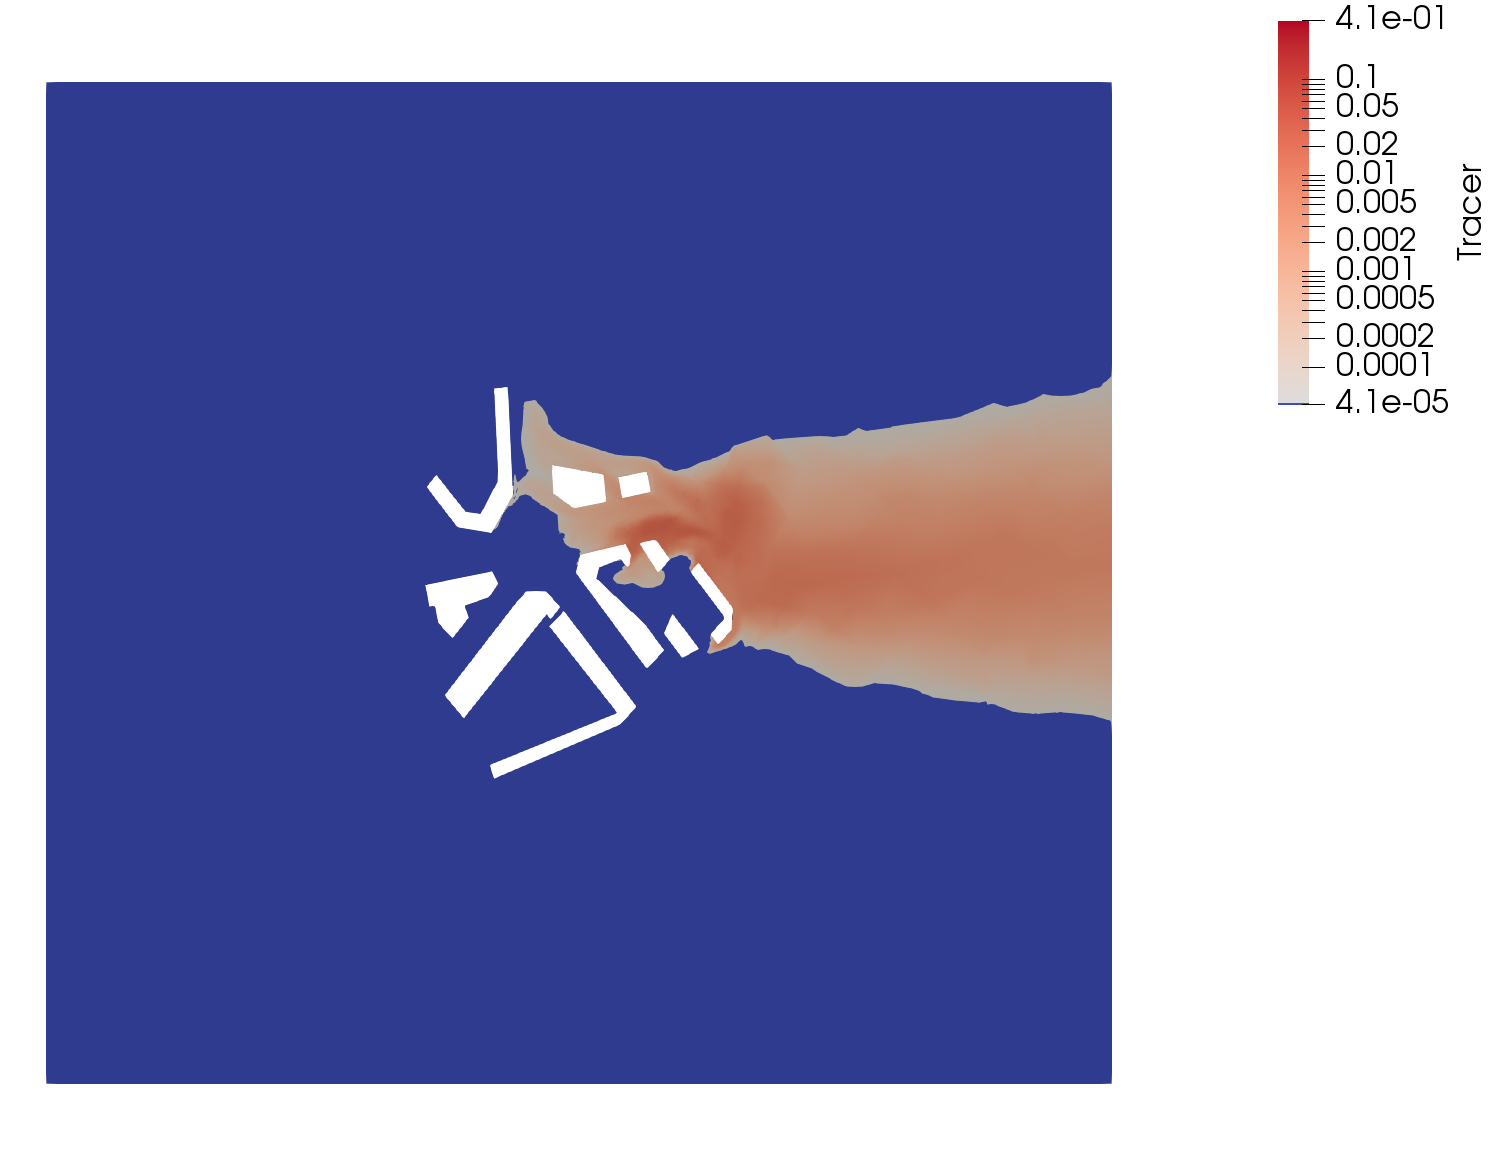
\includegraphics[width=0.8\linewidth]{figures/Analysis/tracer988cutZ1}
  \caption{Tracer Field : Horizontal cut at $z=1m$ and $t=988$}
  \label{fig:view:tracerend}
\end{figure}




The \textbf{tracer} represents the propagation of a pollutant generated from the centre of the domain at ground level. It aims a representing a busy intersection. We represent two horizontal cuts of the tracer field at $z=1m$ and at $t=50$ and $t=988$ in the figures \ref{fig:view:tracerstart} and \ref{fig:view:tracerend}\\




As we can see by observing the time propagation of those fields,  the wind is pushing the pollutants in a certain direction. Because of this, be observe that the \textbf{tracer} concentration is mainly visible downwind. \\


We can also visualise the quantity of zero elements present in the data \textit{in function of the time}. We count every point of data that has a value over $\tau = 10^{-12}$. This gives us the plot of figure \ref{fig:sumtime}. As we can see, it takes some initial time for the tracer to propagate to some kind of steady state, at around 60\% of the points.

\begin{figure}[h]
\centering
	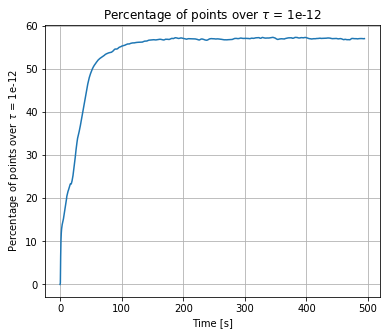
\includegraphics[width = 0.6 \textwidth]{figures/DataAnalysis/SumDataTime}
	\caption{Percentage of significant points in function of the time for $\tau = 10^{-12}$}
	\label{fig:sumtime}
\end{figure}




\section{Preselection of the Data} \label{sec:preselection}
%
%For the purpose of testing our codes and algorithms,  we are going to use a subset of the whole dataset containing a few hundreds to a few thousands of points. 
%
%\todo{rewrite the introduction of this section}
%
%The raw data is contained in VTK files. I have implemented functions in python that allows the importation, the cropping of the space, the extraction of the fields and interest and the location of the points and the saving in files for making quicker the loading procedure. 

As we have seen previously there is a large amount of irrelevant data points inside the original dataset. A lot of points have a tracer concentration close to $0$ and most of relevant points are found downwind of the origin. In this section we are going to see how to remove irrelevant points and in the same time make the dataset smaller and therefore reduce the computational cost of the main optimisation problem. 

\subsection{Selection of a working subset of the data}
The first approach that we have in order to reduce the number of the potential sensor locations, is the reduction of the space in which  we run our optimisation problem. We are focusing on the \textit{tracer} field of the simulation data. This field contains the propagation of a pollutant originating at the \textbf{center of the space} and under wind conditions blowing in the \textit{east direction} (see figure \ref{fig:view:tracer} ). The resulting data shows that most of the space is unaffected by this pollutant and so we wish to select only the space in which the pollutant concentration is non negligible. For that we develop the following procedure. \\

First we cut our 3D space into cuboids. For that we fix a number of bins per dimension and we obtained $R$ subsets $\{\mathcal{D}_k\}_{k=0}^R $. For each subspace we compute the sum over time and space of the tracer values $Y_t^i$  : 

\begin{equation}
	C(\mathcal{D}_i) = \sum_{k \in \mathcal{D}_i} \sum_{t = 0}^T Y_t^k
\end{equation}

We apply then a selection of the subsets based on the value of $C(\mathcal{D}_i)$ and a  threshold $\tau$. We keep then every subset $\mathcal{D}_i$ that respects the condition : $C(\mathcal{D}_i) > \tau$. This condition but guarantees that the points kept in the new working subset $S$ have a sufficient importance in the physical world. The new working subset for our optimisation problem would then be : 

\begin{equation}
	S = \bigcup_{C(\mathcal{D}_i) > \tau} \mathcal{D}_i
\end{equation} 

An example of this algorithm is now explained. For a number of bins of 25 in each dimension and threshold of $\tau = 10^{-2}$ we obtain a new working set size $|S| = 57'725$ instead of an original number of $100'040$. It is displayed on the figure \ref{fig:working_subset}


\begin{figure}[h]
\centering
	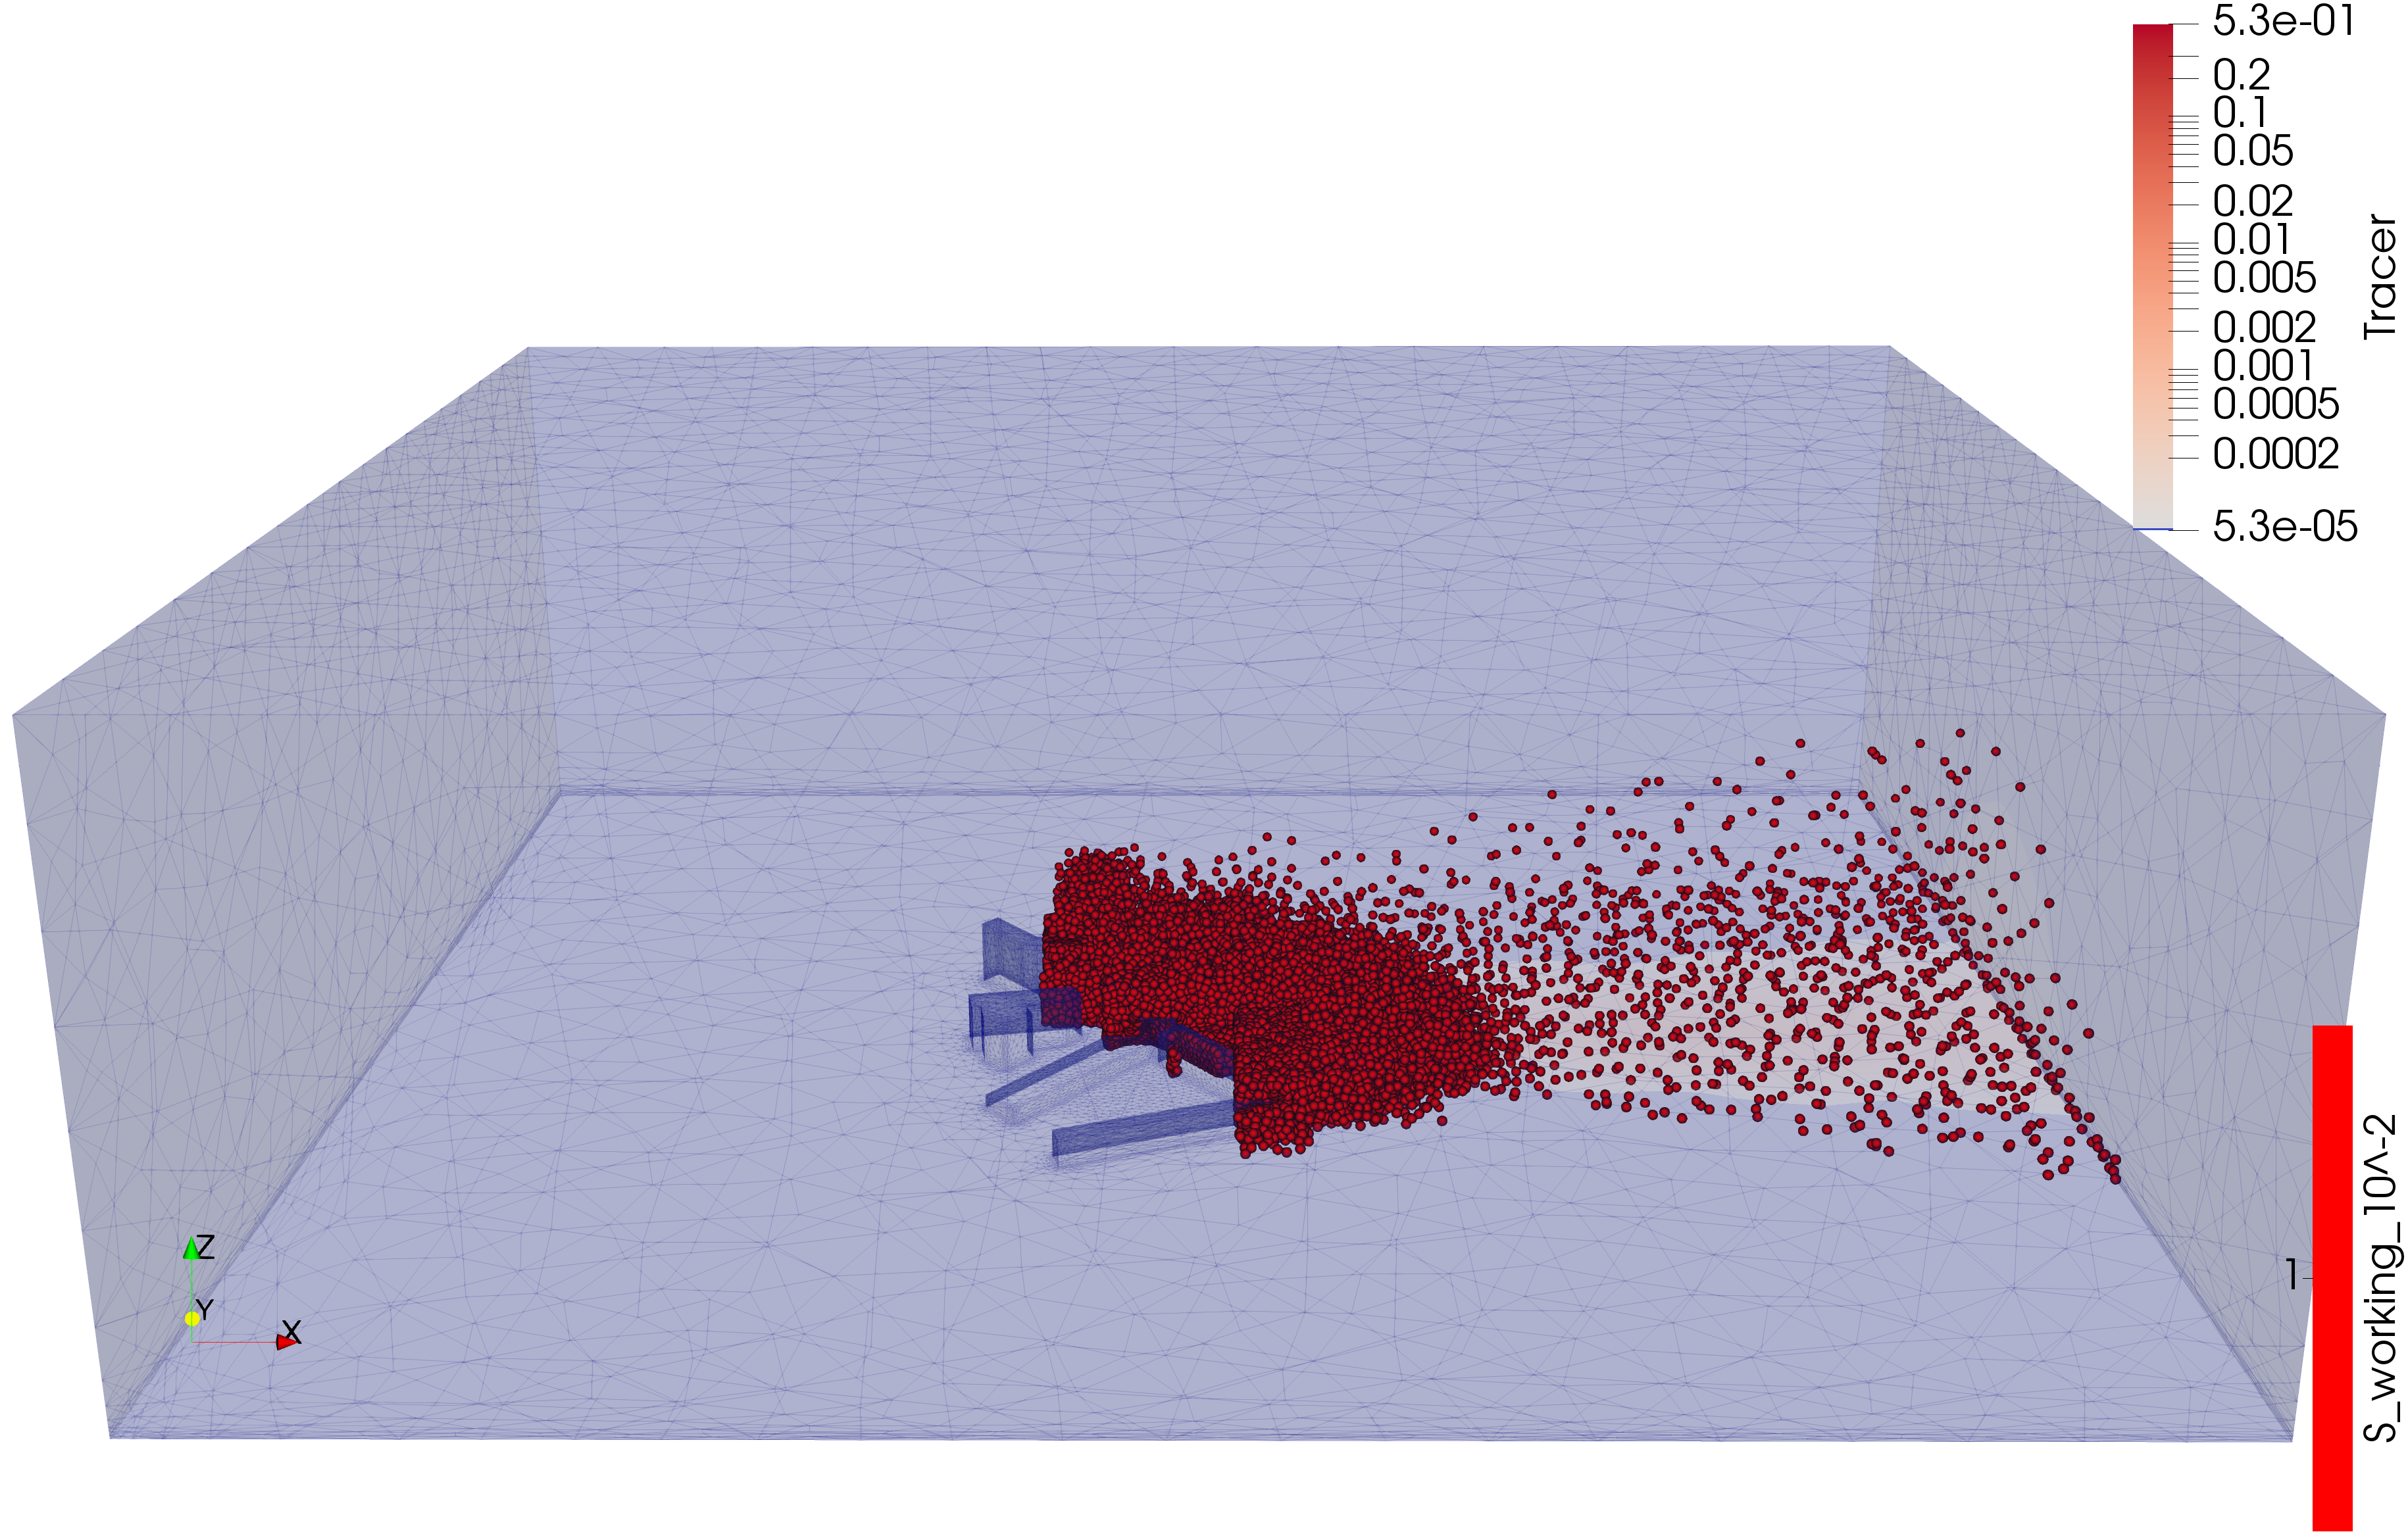
\includegraphics[width = 0.8 \textwidth]{figures/Subset/working_subset_10^-2}
	\caption{New working subset $S$ for $\tau = 10^{-2}$}
	\label{fig:working_subset}
\end{figure}

\subsection{Selection of a subset at human level}

In order to further reduce the number of points involved in the optimisation problem, we can also consider taking points that are only \textbf{accessible by a human from the ground level or the buildings}. This makes sense in the way that sensors needs to be reached from the ground and the  building top and sides for their initial placement and maintenance. \\

We define for each building $i \in \{1, \dots, B\}$ an altitude $H_i$, and for $i = 0$ we consider the rest of the unoccupied space, so $H_0 = 0$. This allows us to define an altitude under which we will select the points : $H_i + h$. The area covered by the buildings is enlarged by the value $w$, so that is covers also the sides of the buildings. See the illustration provided in figure \ref{fig:humanchart}. \\

\begin{figure}[h]
\centering
	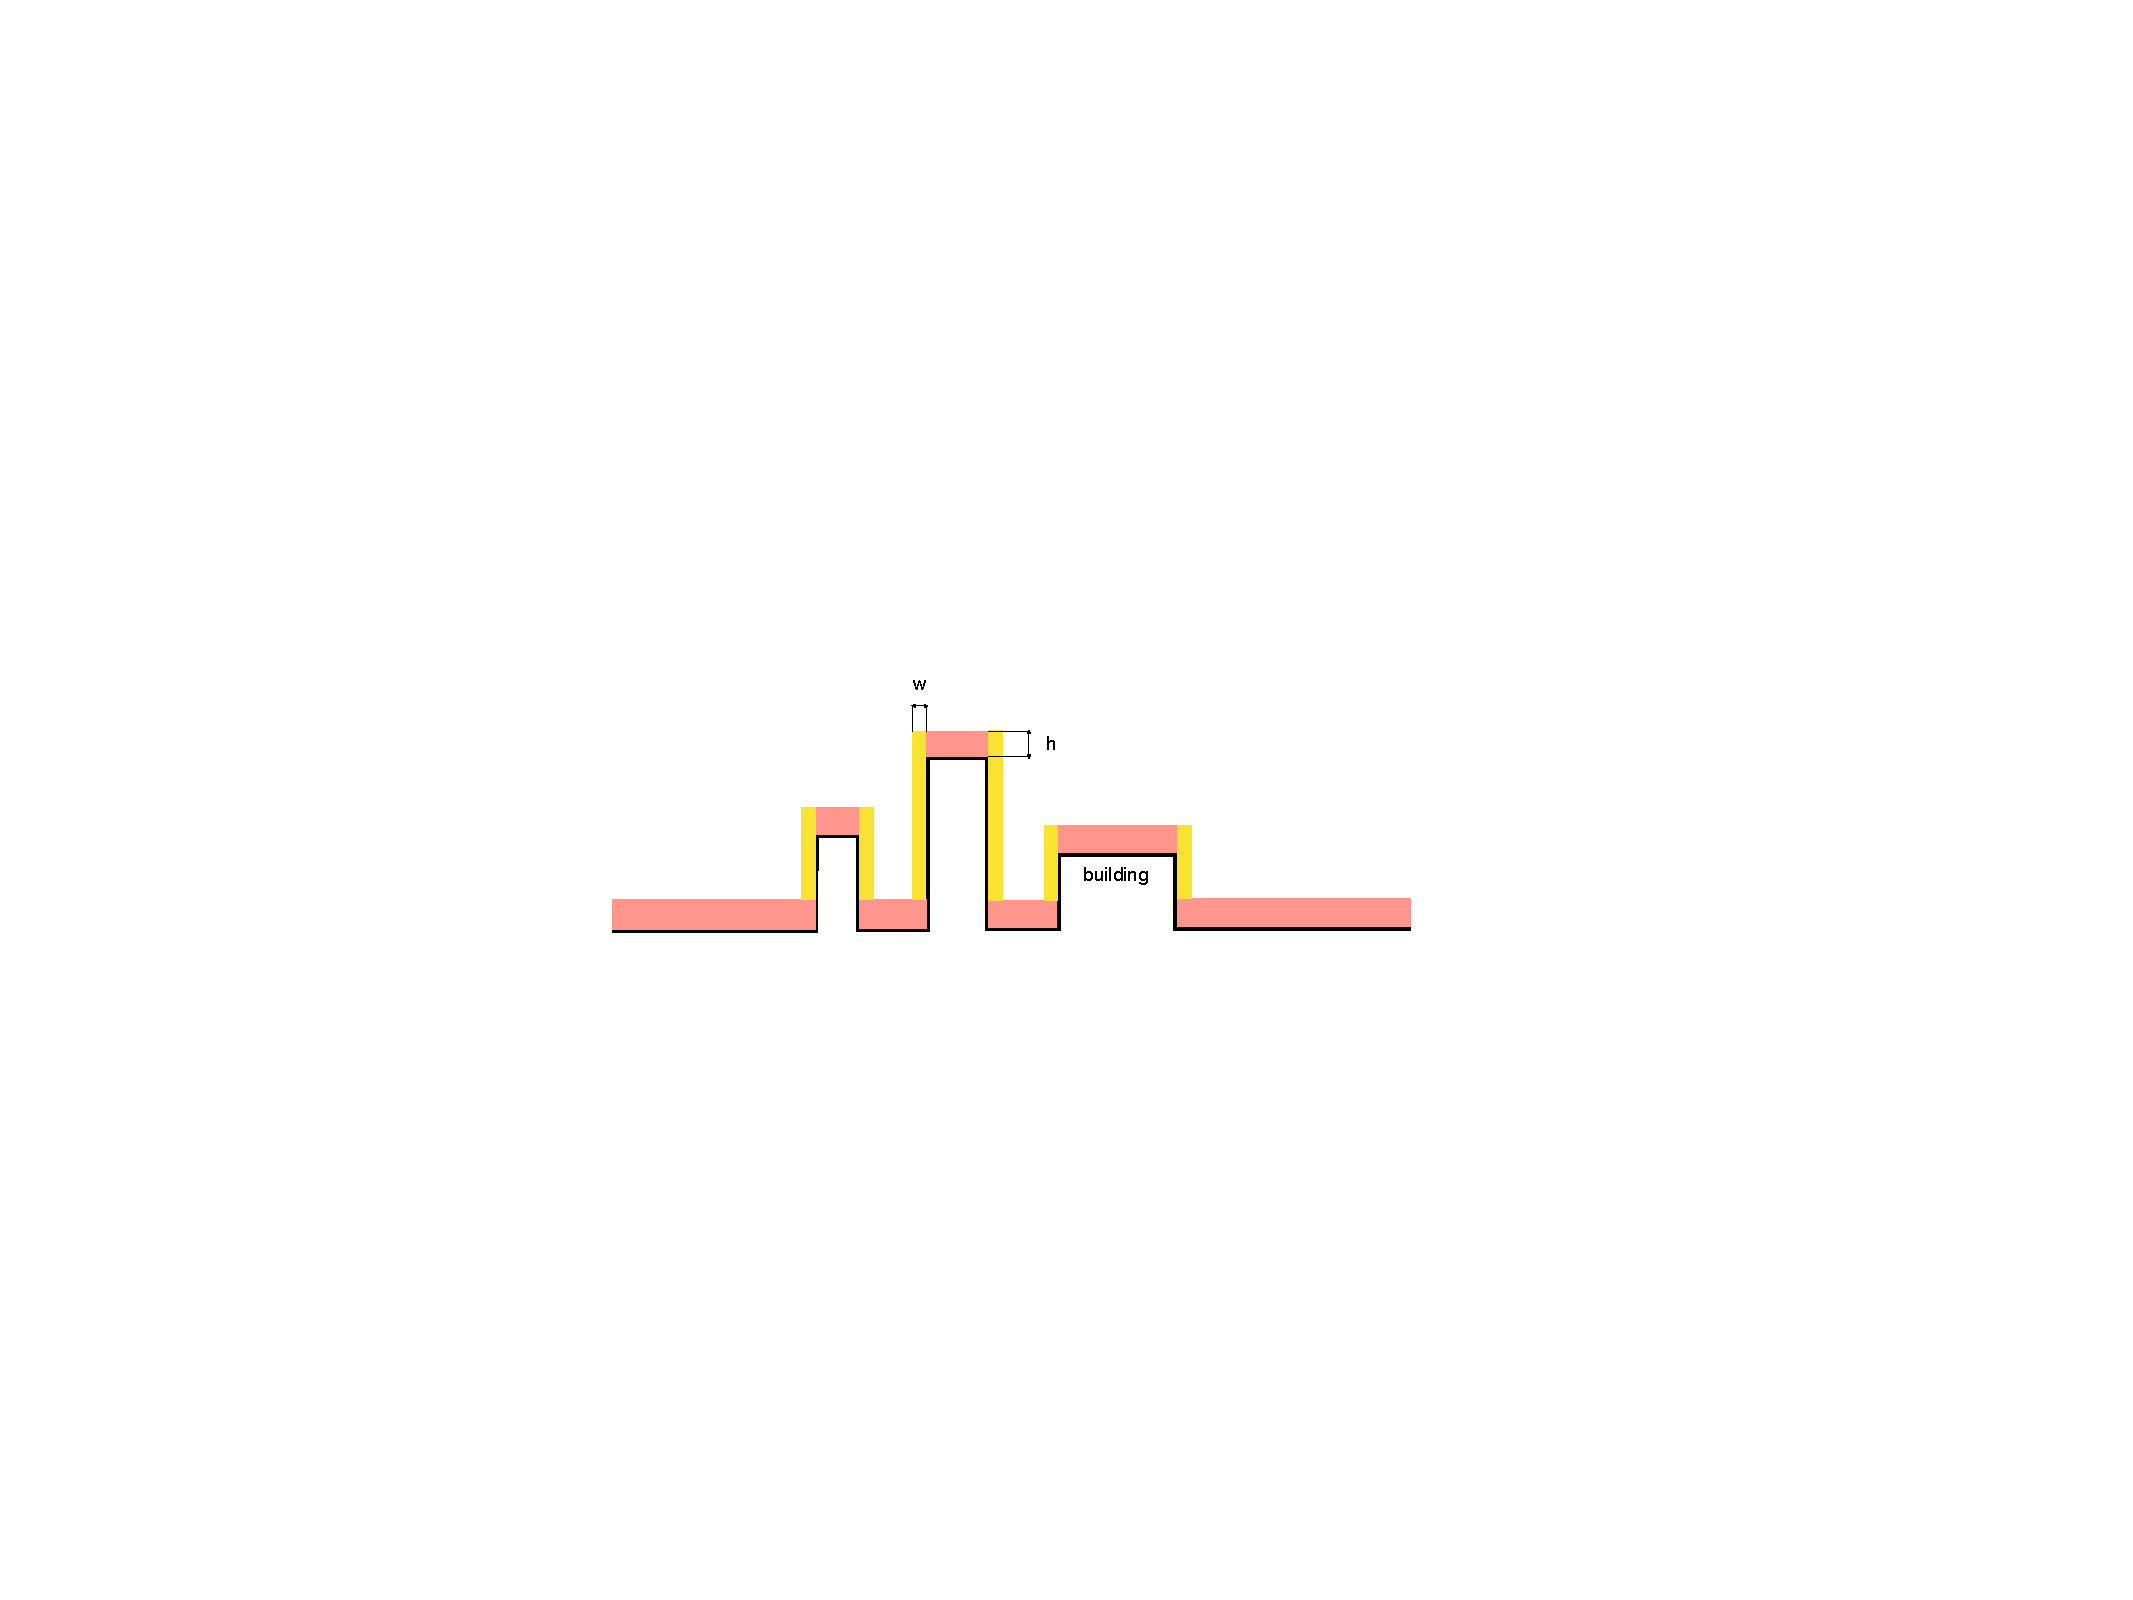
\includegraphics[width = 0.6 \textwidth]{figures/Subset/HumanSelection_chart}
	\caption{Chart Presenting the Building Profile in Human Level Selection}
	\label{fig:humanchart}
\end{figure}

In order to proceed to this selection, I had to overcome the absence of defined building profile and I had to manually define the shapes of the buildings (as you can see on figure \ref{fig:buildingshapes}) by taking the empirically the coordinates of the buildings in the small LSBU dataset, considering a XY projection of the 3D space. \\

\begin{figure}[h]
\centering
	
\includegraphics[width = 0.25 \textwidth]{figures/Subset/buildingShapes_13}
	\caption{Empirical Building Shapes}
	\label{fig:buildingshapes}
\end{figure}

Once those coordinates acquired, I used the \textbf{shapely} library  \citep{noauthor_shapely_2019} in order to define the polygones associated to the buildings. In order to define the height $H_i$ of each building I had to define a set of points overhanging it and find the minimal altitude of this point.  To define the set of points I took the inner part of the surface of the building (cut by 1m) in order to avoid any edge point. This can be seen on the figure \ref{fig:inner_outer_building}). The points which have XY coordinates within this shape are then selected and the minimal Z coordinate is taken as the definition of the roof level $H_i$ \\


\begin{figure}[h]
\centering
	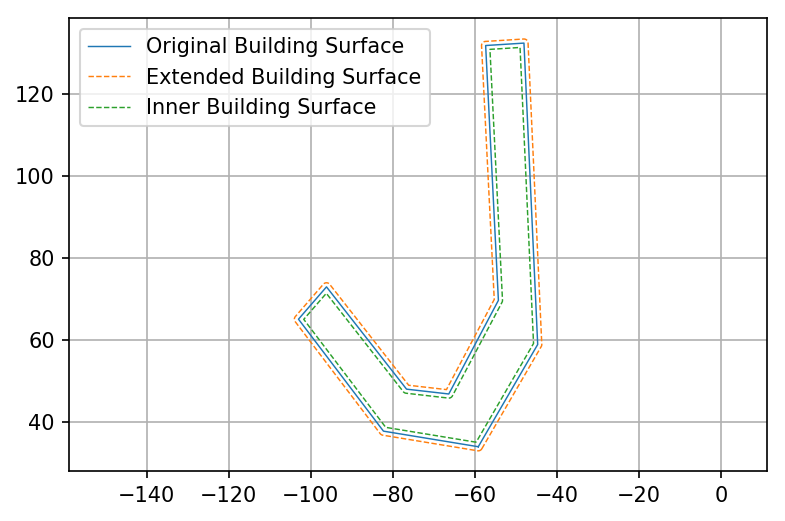
\includegraphics[width = 0.7 \textwidth]{figures/Subset/BuildingSurfaceBuffer}
	\caption{Extended an Inner building surface}
	\label{fig:inner_outer_building}
\end{figure}

Once the roof level defined we come back to the original shape of the building and enlarge it of $w$ such as showed in figure \ref{fig:inner_outer_building}. We then select every point of the main dataset that have XY coordinates in this extended rooftop and   choose only the ones which have Z bellow the threshold $H_i + h$. This constitutes our human level data selection. An illustration can be found on figure \ref{fig:human_selection}. \\

\begin{figure}[h!]
\centering
	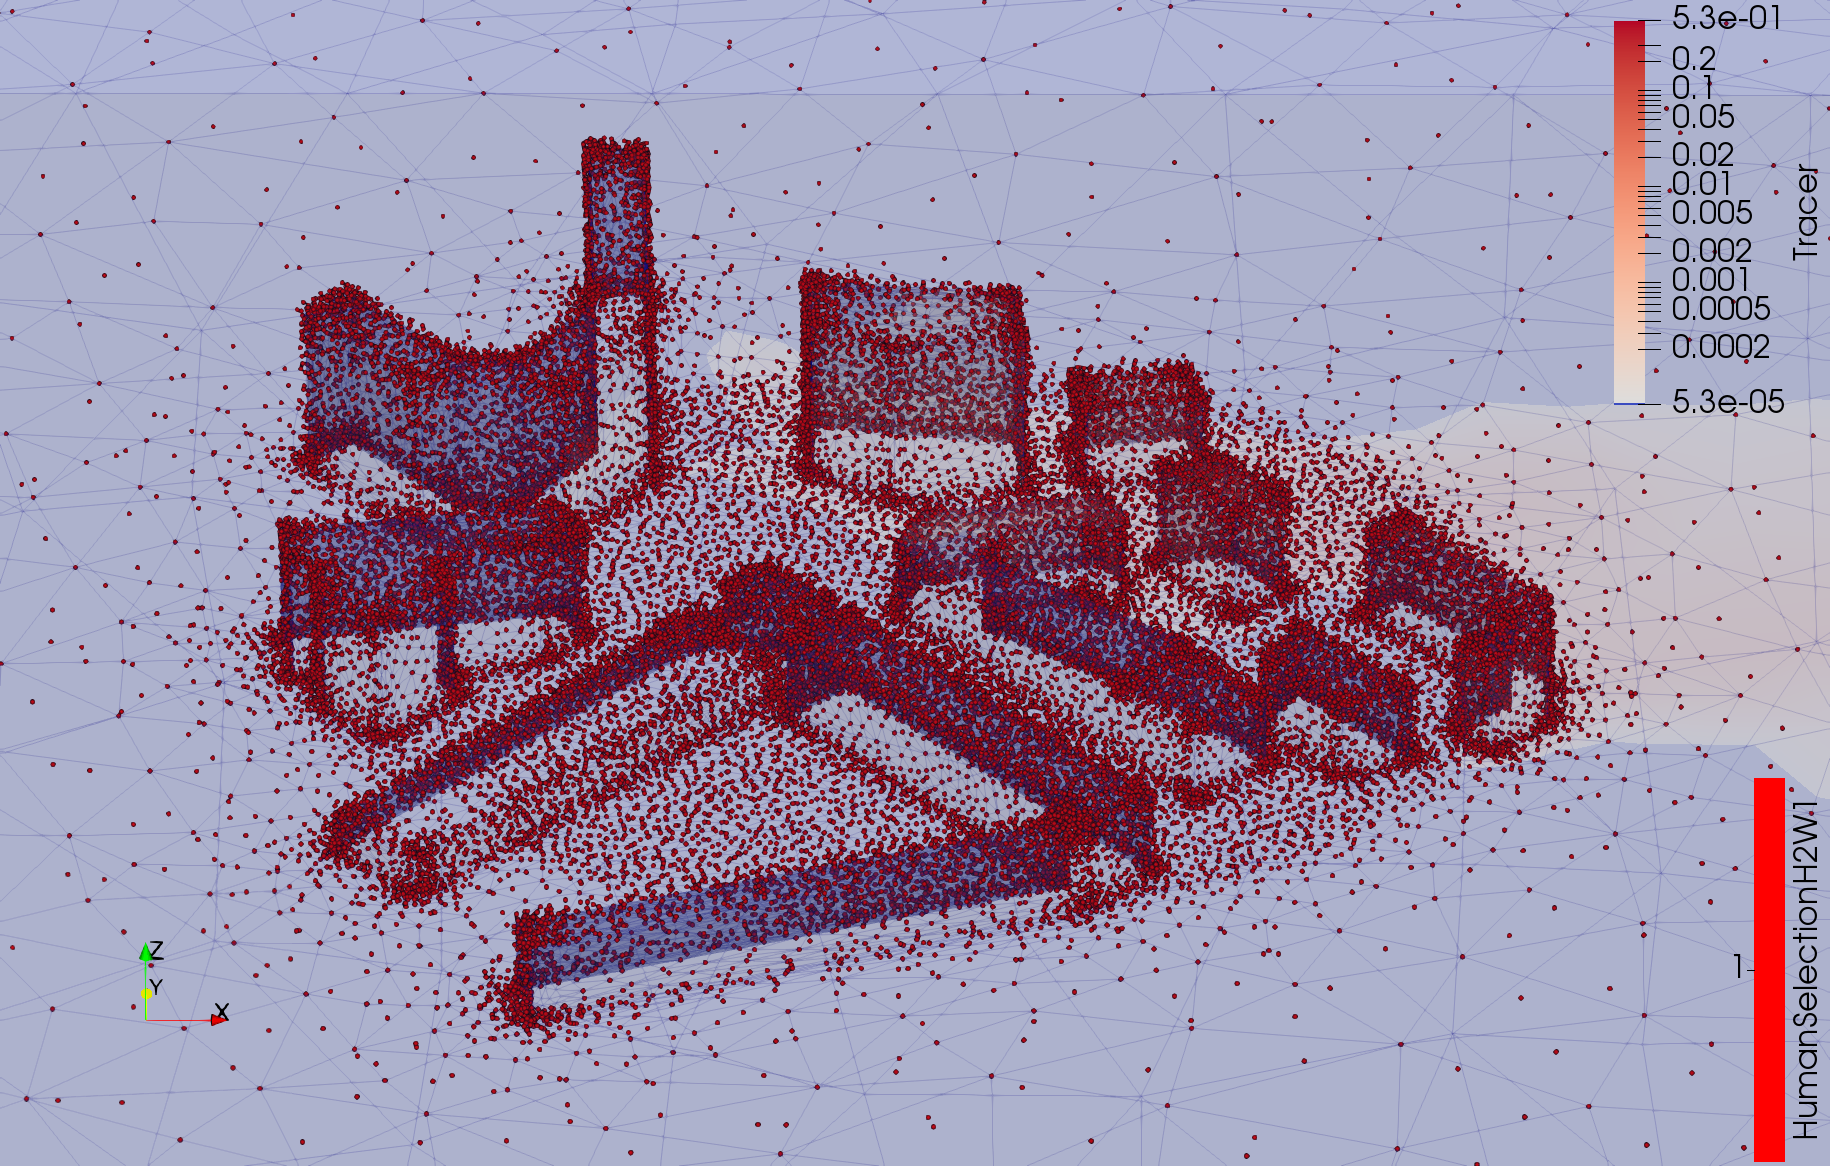
\includegraphics[width = 0.8 \linewidth]{figures/Subset/HumanSelectionH2W1_zoom}
	\caption{Human Level Selection}
	\label{fig:human_selection}
\end{figure}

This method can be seen as quite empirical, but it enables a precise dataset selection with no outlying irrelevant point. \\

With the parameters $h = 2$m and $w = 1$m we reduce the size of the dataset to $|S| = 37'847$. 


\subsection{Combined Selection}

By combining the two selection approaches and by taking the intersection of the two previously defined datasets : the working subset based on the values of the tracer and the human level selection. We are able to reduce the number of points in the dataset to $|S| = 23'643$, instead of an original number of $100'040$, which is a reduction of $76.36\%$ of the original size. In the figure \ref{fig:combined_selection} we see an illustration of the selected dataset that will be used in the rest of the project. 

\begin{figure}[h!]
\centering
	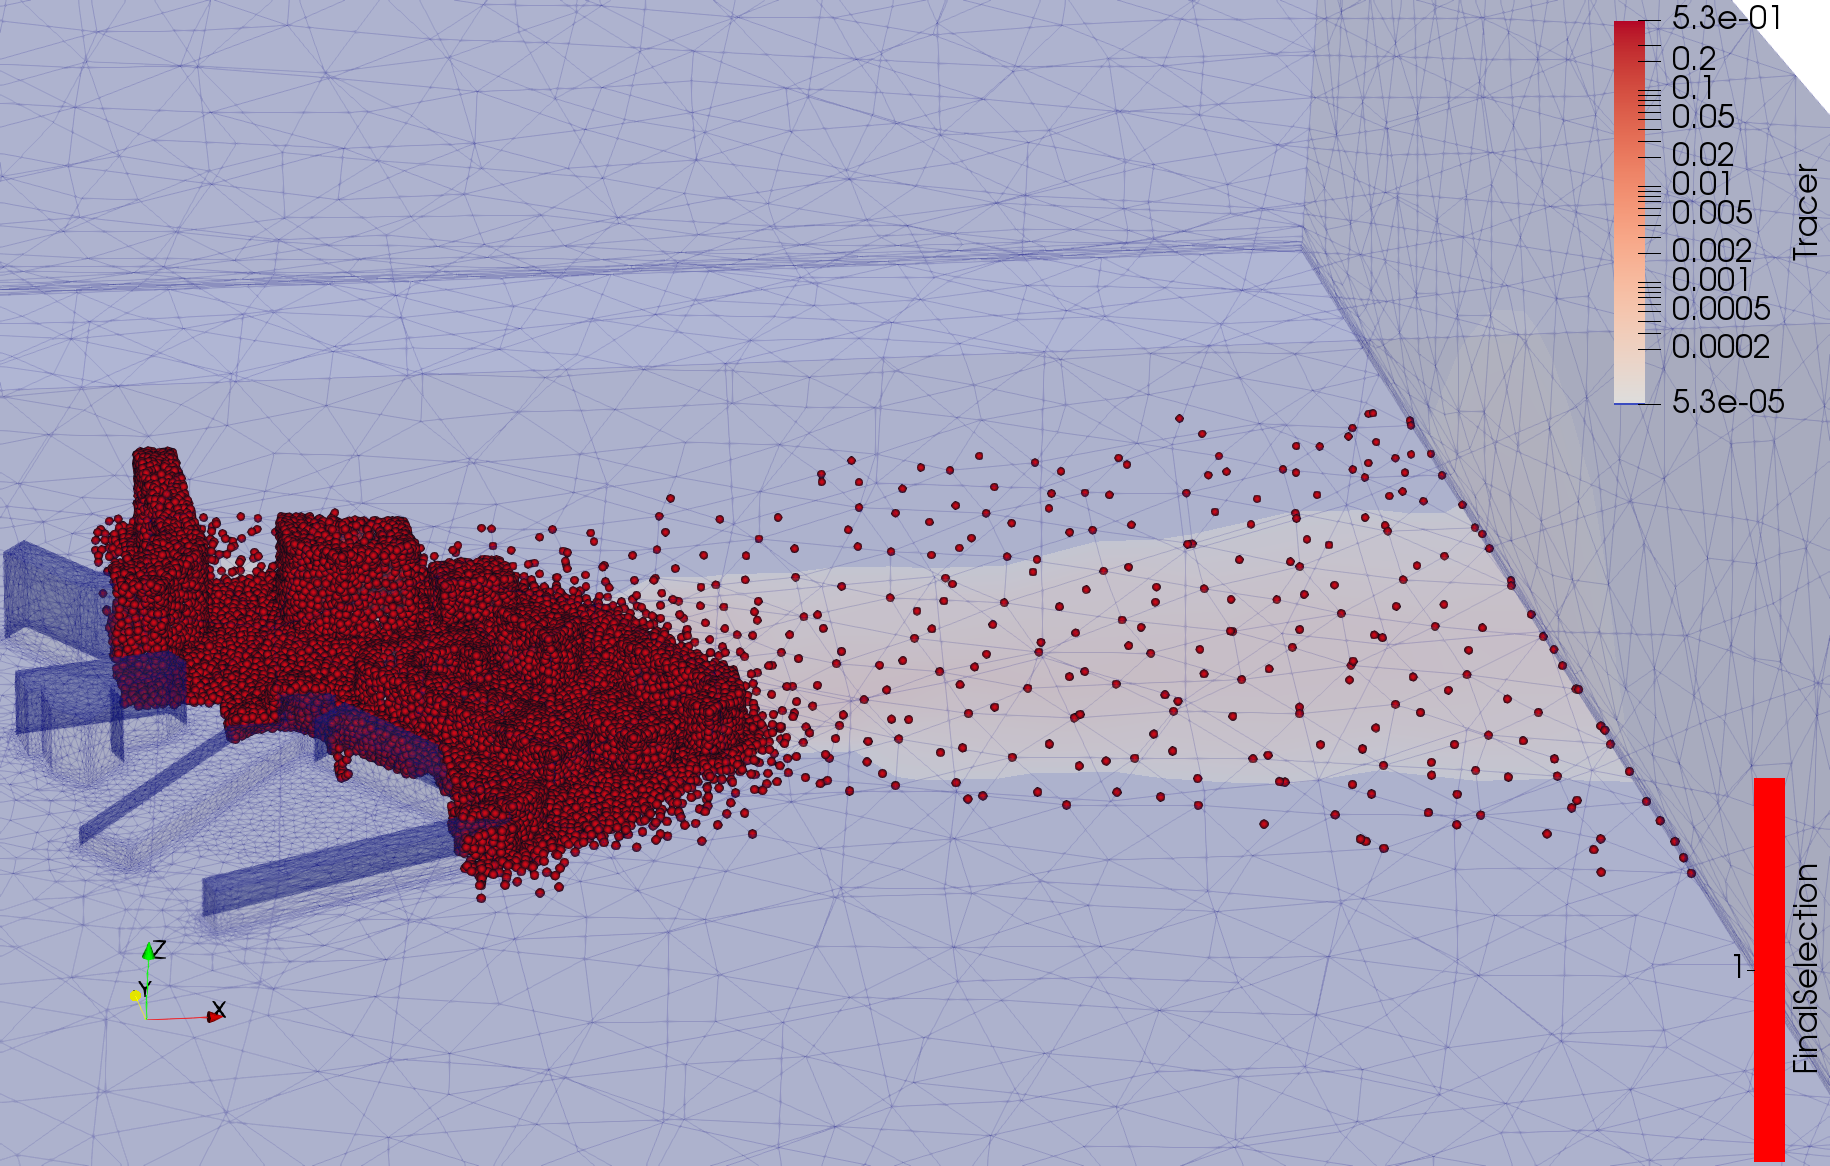
\includegraphics[width = 0.8 \linewidth]{figures/Subset/FinalSelection_zoom}
	\caption{Combined Selection : Working Subset and Human Level Selection}
	\label{fig:combined_selection}
\end{figure}


\section{Implementation of Covariance Matrix}

After the pre-selection of the data, we proceed to the computation of the covariance matrix needed for the optimisation process. This covariance links each point of the space with each other, having the size $23'643 \times 23'643 $.\\

We take advantage of the \textit{sklearn} library that contains a number of useful methods including one computing the Sample Covariance, the LW and the OAS shrinkage estimators. Any parameters used are explained in the chapter \ref{chap:results}. \\



\section{Implementation of Gaussian Processes}

GPs are in fact the main concept used in this project. We will cover here how they were implemented and what king of approximation is was made to make them more scalable. 


\todo{Important to explain how the gaussian processes were implemented. Challenge of the inversion. Classical approach and TSVD approach and show simple computation times and error results.} 

\subsection{Classical GPs}

As we have seen in section \ref{sec:theory:gp}, the gaussian process conditional covariance estimation requires only the knowledge of the covariance matrix $\K$. 

\begin{align}
	\vec{K}_{y | \A} &=  \vec{K}_{yy} - \vec{K}_{y\A} \vec{K}_{\A\A}^{-1} \vec{K}_{\A y} 
\end{align}

The first approach is simply to implement this equation using the \textit{numpy} library. It has the advantage to use parralel processing that exploits the multiple cpus of the computer in order to speed up linear algebra computations, such as this one. 

\subsection{GPs Approximation with TSVD}

In GPs, the inversion of the matrix $\K_{\A\A}$ is the most expensive operation, as it has a complexity of $\mathcal{O}(n^3)$. In to reduce the computational cost of the Gaussian Process, we propose a method that allows to approximate the covariance by reducing the dimension of the data, using the \textbf{truncated singular values decomposition} (TSVD). The idea has been developed by \citep{hansen_truncatedsvd_1987} as it allows to regularise matrix in ill-posed problems.  \\

We recall, the centred data $\vec{X}$ and the sample covariance matrix $\vec{\hat{S}}$. The data $\vec{X}$ has for size $p\times n$ and we would like to approximate it by a matrix of size $\tau \times n $. The singular value decomposition (SVD) allows to express the data matrix as a product of a rectangular diagonal matrix $\vec{\Theta} = \text{diag}(\sigma_1, \dots, \sigma_n ) \in \mathbb{R}^{p \times n} $ containing the singular values, and two orthogonal singular vectors matrices $\vec{V} \in \mathbb{R}^{n \times n} $ and $\vec{U} \in \mathbb{R}^{p \times p} $, such as : 

\begin{equation}
	\vec{X} = \vec{U} \vec{\Theta} \vec{V}^T
\end{equation}

We truncate the SVD from $p$ to $\tau$ by keeping only $\tau$ singular values. We have the singular matrix $\vec{\Theta}_\tau = \text{diag}(\sigma_1, \dots, \sigma_\tau, 0, \dots, 0 ) \in \mathbb{R}^{p \times n} $. We are then able to express an approximation of the data $\vec{\tilde{X}}$ : 

\begin{equation}
	\vec{\tilde{X}}_\tau = \vec{U} \vec{\Theta}_\tau \vec{V}^T
\end{equation}


We apply this approach to the set of points $\A$ with the data $\vec{X}_{\A}$. We get the resulting TSVD for this data : $\vec{\tilde{X}}_{\A,\tau} \in \mathbb{R}^{\tau \times n}$ we can compute with it an approximation of the sample covariance that can be easily inverted and used in our GP based optimisation.

\begin{equation}
	\vec{\tilde{K}}_{\A\A} = \frac{1}{n}\vec{\tilde{X}}_{\A,\tau}  \vec{\tilde{X}}_{\A,\tau}^T
\end{equation}

We also replace the vector of covariance $\vec{K}_{y\A}$ by : 

\begin{equation}
	\vec{\tilde{K}}_{y\A} =  \frac{1}{n}\vec{X}_{y} \vec{\tilde{X}}_{\A,\tau}^T
\end{equation}

We end up with an expression of TSVD approximate GP variance : 

\begin{equation}
	\tilde{\vec{K}}_{y | \A} =  \frac{1}{n} \left( \vec{X}_{y}\vec{X}_{y}^T - \vec{X}_{y} \vec{\tilde{X}}_{\A,\tau}^T (\vec{\tilde{X}}_{\A,\tau}  \vec{\tilde{X}}_{\A,\tau}^T)^{-1}  \vec{\tilde{X}}_{\A,\tau} \vec{X}_{y}^T \right)
\end{equation}

With this approximation the inversion has a complexity reduced to $\mathcal{O}(\tau^3)$, which is a great improvement. \\

 However, this method requires the computation of a new TSVD at each iteration of the algorithm as the indexes in $\A$ are constantly changing. 
 
 \todo{Results add discussion on the cost of TSDV refer to the email}


\subsection{Other Approaches}

A lot of literature was found on how GPs could be made more scalable : approaches relying on very elegant solutions, such as sparse GPs and VFE. After implementing them using specialised GP library (such as \textit{GPy}), I discovered that they could not be applied to our optimisation problem. Sparse GPs are in fact optimisation problems that allow to select a reduced number of positions to represent a large set of observations. But in our algorithm the observation set changes at every step of the of the loop and we need a new approximation for predicting at only one single point. This makes this approach computationally inefficient for the algorithms of \citet{krause_near-optimal_2008}. \\



If we analyse the algorithm \ref{alg:greedy} in more details, we see that it is difficult to implement any sophisitcated method to approximate the GP at each step. \\

We have defined $\A$ as the set of already placed sensors, and $\bar{\A}$ the set of other locations : $\bar{\A} = \mathcal{V} \backslash \{\A \cup y\} $ and $y$ is the candidate point changing at each step. We then have the full set of locations that is cut in 3 parts : $ \mathcal{V} = \A \cup \bar{\A} \cup \{y\} $ \\

At each iteration we need to compute two different GPs. The first one is computing the conditional variance for the point $y$ knowing the set of points $\A$ :   $\vec{K}_{y | \A} =  \vec{K}_{yy} - \vec{K}_{y\A} \vec{K}_{\A\A}^{-1} \vec{K}_{\A y} $. This GP is quite simple to compute as our cardinality of $\A$ is small. Moreover, the covariance matrix  $\vec{K}_{\A\A}$is not changing through the 2nd loop as $\A$ stays the same, so the inversion needs only to be done once. 

The second GP is computing the conditional variance for the point y knowing the set of points $\bar{\A}$ : $\vec{K}_{y | \bar{\A}} =  \vec{K}_{yy} - \vec{K}_{y\bar{\A}} \vec{K}_{\bar{\A}\bar{\A}}^{-1} \vec{K}_{\bar{\bar{\A}} y} $. This is much more difficult to estimate when the number of points in $\bar{\A}$ is of the order of 100’000. Not only it is difficult to estimate once, but be have to to it for every step of the second loop as the set $\bar{\A}$ changes constantly as we move the candidate point $y$. We then have a covariance matrix $\vec{K}_{\bar{\A}\bar{\A}}$ that is fundamentally different between each step. \\

Because of this, if we want to use a method that allows to remove the bottleneck at the covariance matrix inversion, we need to avoid creating another bottleneck to approximate the GP. The TSVD approach is sufficiently light not to increase too much the computational cost. 

\todo{check the last paragraph and maybe move it}





\section{Implementation of the Optimisation}

\todo{Explain every algorithm implemented, their difference. This is important for the result section where sample results for those algorithm will be shown later on }

\subsection{}


The methods developed by \citet{krause_near-optimal_2008} are using the full Gaussian process in to greedily place sensors. The algorithm consists in the estimation of the best “new” sensor to add the set of existing sensor based on a mutual information gain criterion. This criterion can be computed with two Gaussian processes. One that estimates the covariance of the sensor candidate $y$ given the set of previously selected sensors $\A$ : $K_{y | \A}$. The other GP allows the computation of the covariance of the candidate $y$ given the rest of the locations in the space $\bar{\A} = \V \backslash ( \A \cup y )$ : $K_{y | \bar{\A}}$. We recall the problem that is to be solved is :

\begin{equation}
    y^* = {\arg \max}_{y \in \S \backslash A } \: \frac{K_{y | \A}}{K_{y | \bar{\A}}}
\end{equation}

This has to be computed theoretically for every candidate point of the dataset, and this for every sensor we add to A. The naive version is described in \ref{alg:greedy} and a lazy version of the algorithm is available at algorithm \ref{alg:lazy}.


\subsection{Comparison tools : Distance Between Sets}

In order to be able to compare the results of optimisations, we define a metric that can be used to see how close are two optimal sets. \\

The output of our optimisation problem is a set of points $\A$ of size $k$, indexed such as $\A = \{a_1, \dots, a_k\}$. We consider two optimal sets given by two versions of our algorithm : $\A_1$ and $\A_2$. We would to define a metric that measures the distance between those two sets. As we will see several options are possible. \\

We could average the coordinates of the set points and take the $l2$ distance between the averages ($\vec{x}(\cdot)$ being the coordinate of of a point and $\bar{\vec{x}}(\A)$ the average on a set $\A$  ):

\begin{equation}
	d_{av}(\A_1,\A_2) =  \left\lVert \,\bar{\vec{x}}(\A_1)] - \bar{\vec{x}}(\A_1)\, \right\rVert_2
\end{equation}

This is unlikely to measure the spread of the points and how each points is actually close to the other set. This is why we propose to create  a \textbf{nearest neighbour} distance between the points of the sets. \\

First we define a divergence between the sets $\A_1$ and $\A_2$, which takes for each points of $\A_1$ its closest neighbour in $\A_2$, takes the distance between them, and average it across the set. We define a nearest neighbour function $NN(\cdot,\cdot)$ which, given an index $a_i$ in the set $\A_1$ and the set $\A_2$, finds the index in the set $\A_2$ of closest points to $a_i$. This mapping is not bijective and therefore leads to asymmetrical results. 

\begin{equation}
	div_{NN}(\A_1,\A_2) = \frac{1}{k}\sum_{i=1}^k \left \lVert \,\vec{x}(a_i) - \vec{x}(NN(a_i,\A_2))\, \right \rVert_2
\end{equation}

This metric has for unit the meter $[m]$. We also call this metric a \textbf{divergence} as it not \textit{symmetric}. In order to define a distance that is symmetric, we define as follows the \textbf{nearest neighbour distance} :

\begin{equation}
	d_{NN}(\A_1,\A_2) = \frac{1}{2} (div_{NN}(\A_1,\A_2) + div_{NN}(\A_2,\A_1))
	\label{equ:distNN}
\end{equation}

This metric has the advantage of being symmetric, taking into account the distance from each point of the dataset and therefore give a meaningful interpretation of how close are spatially the sets from each other. 
%\paragraph{Computational Time}
%
%An other tool that is going to be used in order to compare the algorithm is the measurement of the computation time for each resolution of the optimisation problem. 





\section{Implementation of VarDA}

\todo{Write this in the end only if the validation works well}
\todo{Explain why only on full set and not on comparison set}





%%%%%%%%%%% CHAPTER: RESULTS
\chapter{Analysis and Results} \label{chap:results}


After analysing the dataset and implementing the optimisation algorithms, we have run several experiments to find the near-optimal points. For that, we have explored different approaches for estimating the covariance function; we have compared the different algorithm on a subset of the data;  we have run the optimisation on the full dataset; and finally, we have applied those results to a Data Assimilation Procedure. 


%%%%%%%%% COVARIANCE %%%%%%%%
\section{Covariance}

As we have seen, our approach relies heavily on a properly defined covariance estimation. We have applied several methods to find a good covariance and we are presenting them in this section. \\

From now on, we will consider that the full dataset is our pre-selected subset with $23'643$ locations. 

%\subsection{Tracer Concentration Covariance}
\subsection{Sample Covariance}

The simplest covariance estimation is the Sample (Empirical) Covariance. This Matrix is a very poor estimate, as it is singular and not positive definite and poorly conditioned. It makes it impossible to invert to use it for the GPs of our optimisation problem. \\ 

We compute the determinant of the matrix using \texttt{numpy.linalg.slogdet} for the stability of this function. It indicates us that the determinant is clearly negative, and the logarithm of the determinant's absolute value is: $-1'399'936.286$. The largest eigenvalue is: $\lambda_1 = 0.0219$ and the smallest eigenvalue is: $\lambda_p = -6.8929 \cdot 10^{-18}$.

We plot in Figure \ref{fig:cov:emp:eigs} the eigen-decomposition of this sample covariance matrix.

\begin{figure}[h!]
\centering
    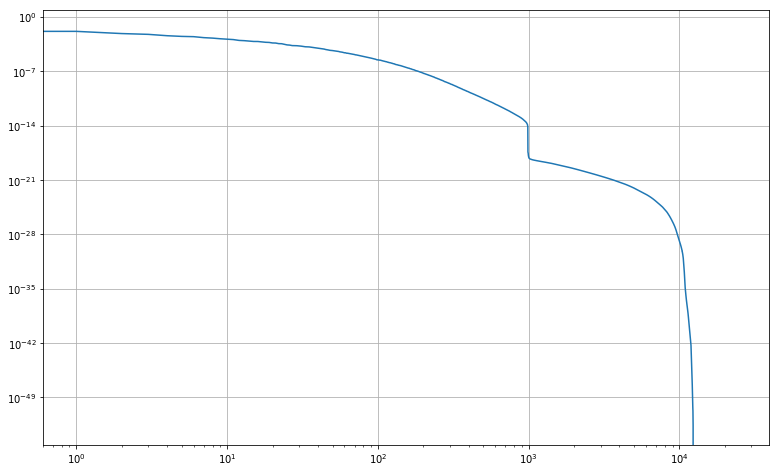
\includegraphics[width=0.7\linewidth]{figures/Covariance/Tracer_23643/cov_emp_eigenval_loglog}
    \caption{Empirical Covariance: Eigenvalues - Tracer}
    \label{fig:cov:emp:eigs}
\end{figure}

So the sample covariance matrix can not be directly used for our optimisation algorithm.  

\subsection{Shrinkage Covariance}

In this section we show the results of the class of shrinkage covariance estimators for the \textit{Tracer} Data. We use a simple \textbf{shrinkage} with shrinkage constant $\rho = 0.1$,  $\rho = 0.5$ and $\rho = 0.8$,  the \textbf{Ledoit-Wolf} Shrinkage and the \textbf{OAS} Shrinkage. 

\begin{table}[h]
\centering
    \begin{tabular}{l|ccccc}
     \toprule
        & SignDet & LogDet & $\lambda_1$ & $\lambda_p$ & $\rho$ \\ \midrule
        Empirical & ($-$) & $-1'399'936.28$ &  $0.0219$ & $-6.8929 \cdot 10^{-18}$ & -\\
        Shrinkage $\rho=0.1$ & ($+$) & $-351'807.64$ &  $0.0197$ &$3.3603\cdot 10^{-7}$ & $0.1$\\
        Shrinkage $\rho=0.5$ & ($+$) & $-314'035.58$ &  $0.0109$  &$1.6801 \cdot 10^{-6}$ & $0.5$\\
        Shrinkage $\rho=0.8$ & ($+$) & $-303'046.20$ &  $0.00438$  &$2.6882 \cdot 10^{-6}$ & $0.8$\\
        Ledoit-Wolf & ($+$) & $-406'320.19$&  $0.0217$ & $3.2867\cdot 10^{-8}$ & $0.0097811$\\
        OAS & ($+$) & $-408'903.33$ & $0.0217$ & $2.9435\cdot 10^{-8}$ & $0.0087595$ \\  \bottomrule
    \end{tabular}
    \caption{Shrinkage Comparison - Tracer}
\end{table}

\begin{figure}[h!]
\centering
    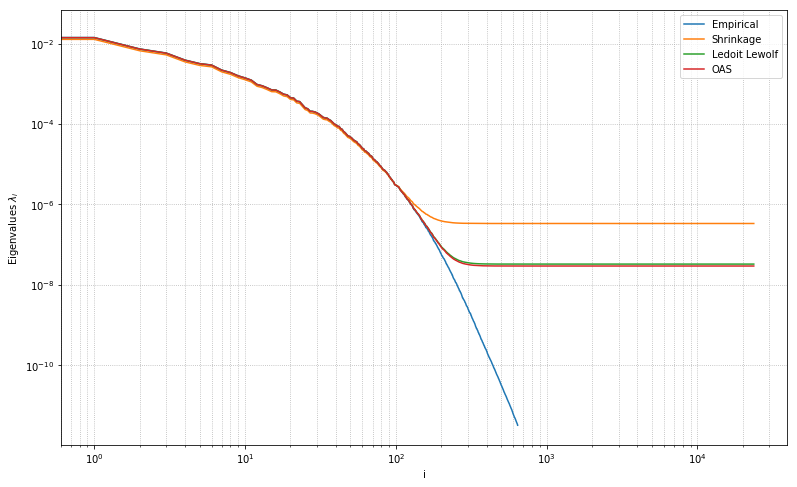
\includegraphics[width=0.8\linewidth]{figures/Covariance/Tracer_23643/cov_all_eigenval_loglog_zoom}
    \caption{Eigenvalues Covariance Comparison - Tracer}
    \label{fig:cov:comparison:eigs}
\end{figure}

As we can see the shrinkage algorithm allows to have a positive definite matrix that is very close to the original covariance matrix. It shares a lot of eigenvalues with the sample covariance matrix. This varies in function of the shrinkage constant $\rho$. For arbitrary values, $\rho = 0.1$,  $\rho= 0.5$ and  $\rho= 0.8$, we see that the smaller the shrinkage constant is, the closer we get to the sample covariance. For large constant value, we see that the upper part of the spectrum deteriorates completely, meaning that we don't have a good estimation anymore. This is perfectly logical with regards to the definition of the shrinkage which is a convex linear combination between a diagonal matrix and the sample covariance. \\

For LW and OAS, the shrinkage variable computed is close to $0.1$. The spectrums are almost identical and are resulting in very similar covariances matrixes. We see that the upper part of the spectrum is almost identical to the sample covariance matrix, but that the lower part is truncated. \\


Globally, we see that with shrinkage  the small eigenvalues get larger and that the large ones get smaller. We observe also that the determinant becomes positive, and also that it leads to a positive definite matrix. \\

As OAS gives us theoretically an optimal $\rho$ with very small error, therefore, we decide to use the \textbf{OAS estimation} of the covariance matrix for the optimisation procedure to follow.

%\subsection{Covariance on other fields}

%\subsection{Pressure Covariance}
%
%Now we study the same Covariance Estimators applied to the Pressure Field. 
%
%
%\subsubsection{Sample Covariance}
%
%Similarly, we see that the sample covariance matrix is a poor estimate of the true covariance matrix as it is not positive definite and near singular. 
%
%\begin{figure}[h!]
%\centering
%    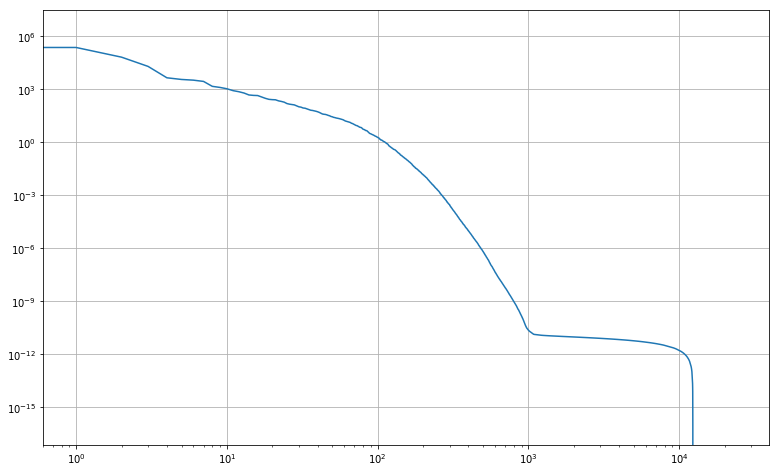
\includegraphics[width=0.8\linewidth]{figures/Covariance/Pressure_23643/cov_emp_eigenval_loglog}
%    \caption{Empirical Covariance: Eigenvalues - Pressure}
%    \label{fig:cov:emp:eigs}
%\end{figure}
%
%\subsubsection{Shrinkage Covariance}
%
%In this section we show the results of the class of shrinkage covariance estimators for the \textit{Tracer} Data. We use a simple \textbf{shrinkage} with shrinkage constant $\rho = 0.8$,  the \textbf{Ledoit-Wolf} Shrinkage and the \textbf{OAS} Shrinkage. 
%
%\begin{table}[h]
%\centering
%    \begin{tabular}{l|ccccc}
%     \toprule
%        & SignDet & LogDet & $\lambda_1$ & $\lambda_p$ & $\rho$ \\ \midrule
%        Empirical & ($-$) & $-601'246.12$ &  $2'303'868.81$ & $-8.0587 \cdot 10^{-10}$ & -\\
%        Shrinkage $\rho=0.8$ & ($+$) & $106330.01$ &  $460'863.34$  &$89.5867$ & $0.8$\\
%        Ledoit-Wolf & ($+$) & $6830.41$&  $2'276'858.60$ & $1.3129$ & $0.01172$\\
%        OAS & ($+$) & $-31'175.97$ & $2'298'501.89$ & $0.2608$ & $0.0087595$ \\  \bottomrule
%    \end{tabular}
%    \caption{Shrinkage Comparison - Pressure}
%\end{table}



%%%%%%%%% COMPARISON %%%%%%%%

\section{Comparison Optimisation Algorithms}

We have defined the three algorithms allowing for a near-optimal placement of the sensors. We have also defined an approximation of the GPs. To compare their performance and measure their limitation, we have run them on a small dataset, a subset of our main one. 
\subsection{Conditions of the Experiment}

We have defined a sphere of radius $25$m, centred close to the centre, in the middle of the propagation beam, at position $[60,35,0]$ in which are contained $3'130$ points of the mesh. By taking the intersection between those points and our selection defined in \ref{sec:preselection}, we can reduce the number of points $|S|$ to $1'295$.  The candidates are presented in Figure      \ref{fig:smallset:position}.
 \\

\begin{figure}[h!]
\centering
    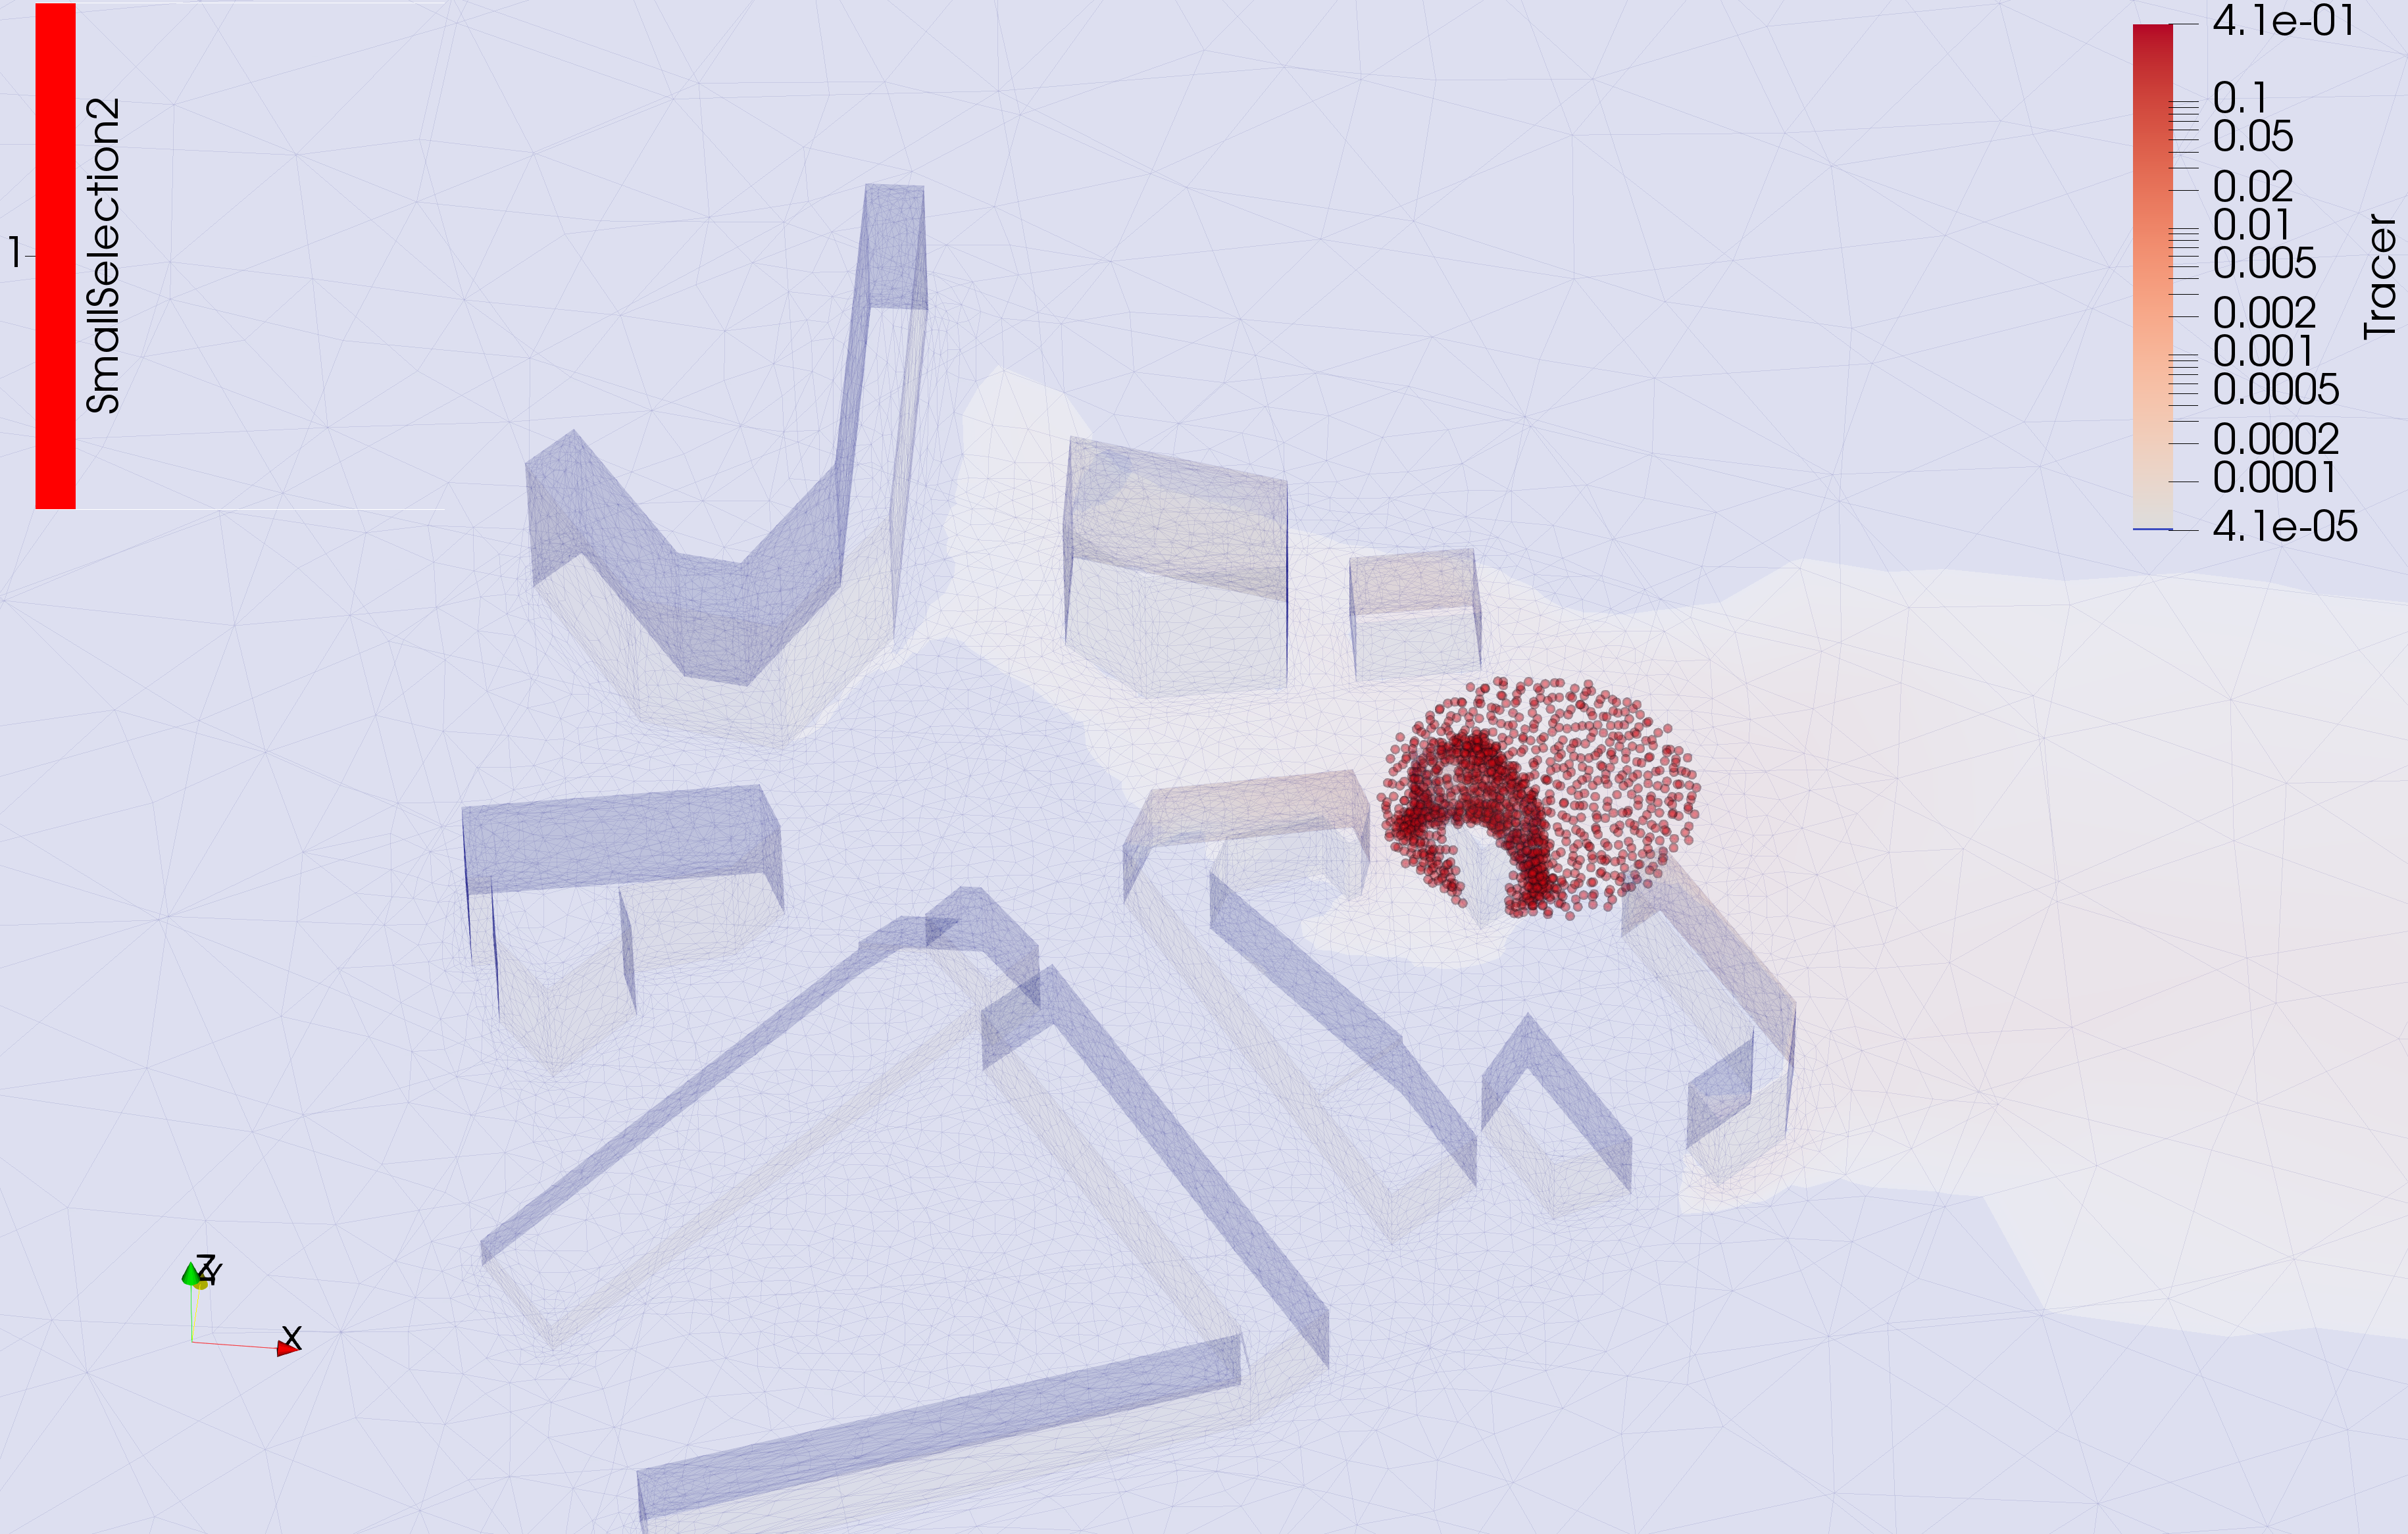
\includegraphics[width=0.8\linewidth]{figures/CompAlg/3rd/non_centered_60.35.0/candidates_screenshot}
    \caption{Small Subset Candidates}
    \label{fig:smallset:position}
\end{figure}

We compute the OAS covariance for this dataset and we will use in in the rest of the experience. The eigenvalues decomposition is shown for both the empirical covariance and the OAS estimate in Figure \ref{fig:small_cov_eig:tracer}. As shown previously we have a spectrum that is close to the original sample covariance,  only with a truncated lower part. \\

For the \textit{Tracer} we have a sample covariance that is \textbf{negative definite} with \textit{logDet} of $-39'755.06$. The OAS approximation allows us to get a \textbf{positive definite} covariance matrix with \textit{logDet} of $-19'447.95$.  \\

%For the \textit{Pressure} we have a sample covariance that is \textbf{negative definite} with \textit{logDet} of $-28'714.93$. The OAS approximation allows us to get a \textbf{positive definite} covariance matrix with \textit{logDet} of $-2'138.49$.  \\

\begin{figure}[h!]
\centering
    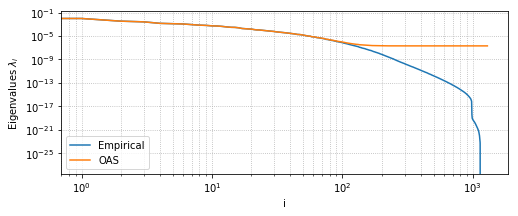
\includegraphics[width=0.7\linewidth]{figures/CompAlg/covarianceEmpOAS}
    \caption{Spectrum of Empirical and OAS covariances for Tracer}
    \label{fig:small_cov_eig:tracer}
\end{figure}

%\begin{figure}[h!]
%\centering
%    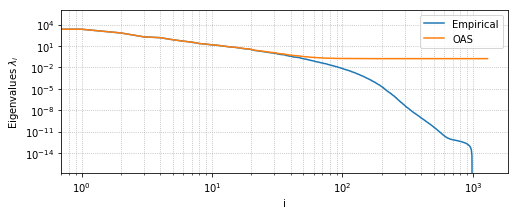
\includegraphics[width=0.7\linewidth]{figures/CompAlg/cov_emp_oas_log}
%    \caption{Spectrum of Empirical and OAS covariances for Pressure}
%    \label{fig:small_cov_eig:pressure}
%\end{figure}

Next, we are going to optimise in this space $k=10$ points with the different algorithms and compare them based on the computation time and the distance between the datasets using the NN distance defined in \ref{equ:distNN}. 

%\subsection{Optimisation on Tracer Concentration}
%In the first time, we are going to compare the performances of the different algorithms using the \textbf{Tracer Concentration} Data. 


\subsection{Greedy and Lazy Optimisation}

First, we optimise using the two first algorithms, the \textbf{greedy} and the \textbf{lazy} versions of the near-optimal sensor positioning algorithms. We will consider the output of the first algorithm as the reference for this comparison. This is because the first algorithm is the most reliable version as it covers every candidate point in its loops and relies on full GP implementation.  \\


We observe immediately that output sets given by the two methods are the same. The main difference is as expected the computation time which is much larger in the first algorithm. The Greedy Optimisation gives a result after $1043.27$s and the \textit{lazy} Optimisation gives results after $153.51 $s. The second algorithm is, for this small dataset, seven times faster than the greedy one: this is a significative difference. \\ 

The location of those points optimal points $\A^*$ is shown in green in the Figure \ref{fig:opt_small} and table \ref{tab:opt_small}. We observe that the points are well spread across space and along the wind direction. As the wind is propagating the tracer concentration, it makes sense that the sensors must be placed along this direction. \\

\begin{figure}[h!]
\centering
    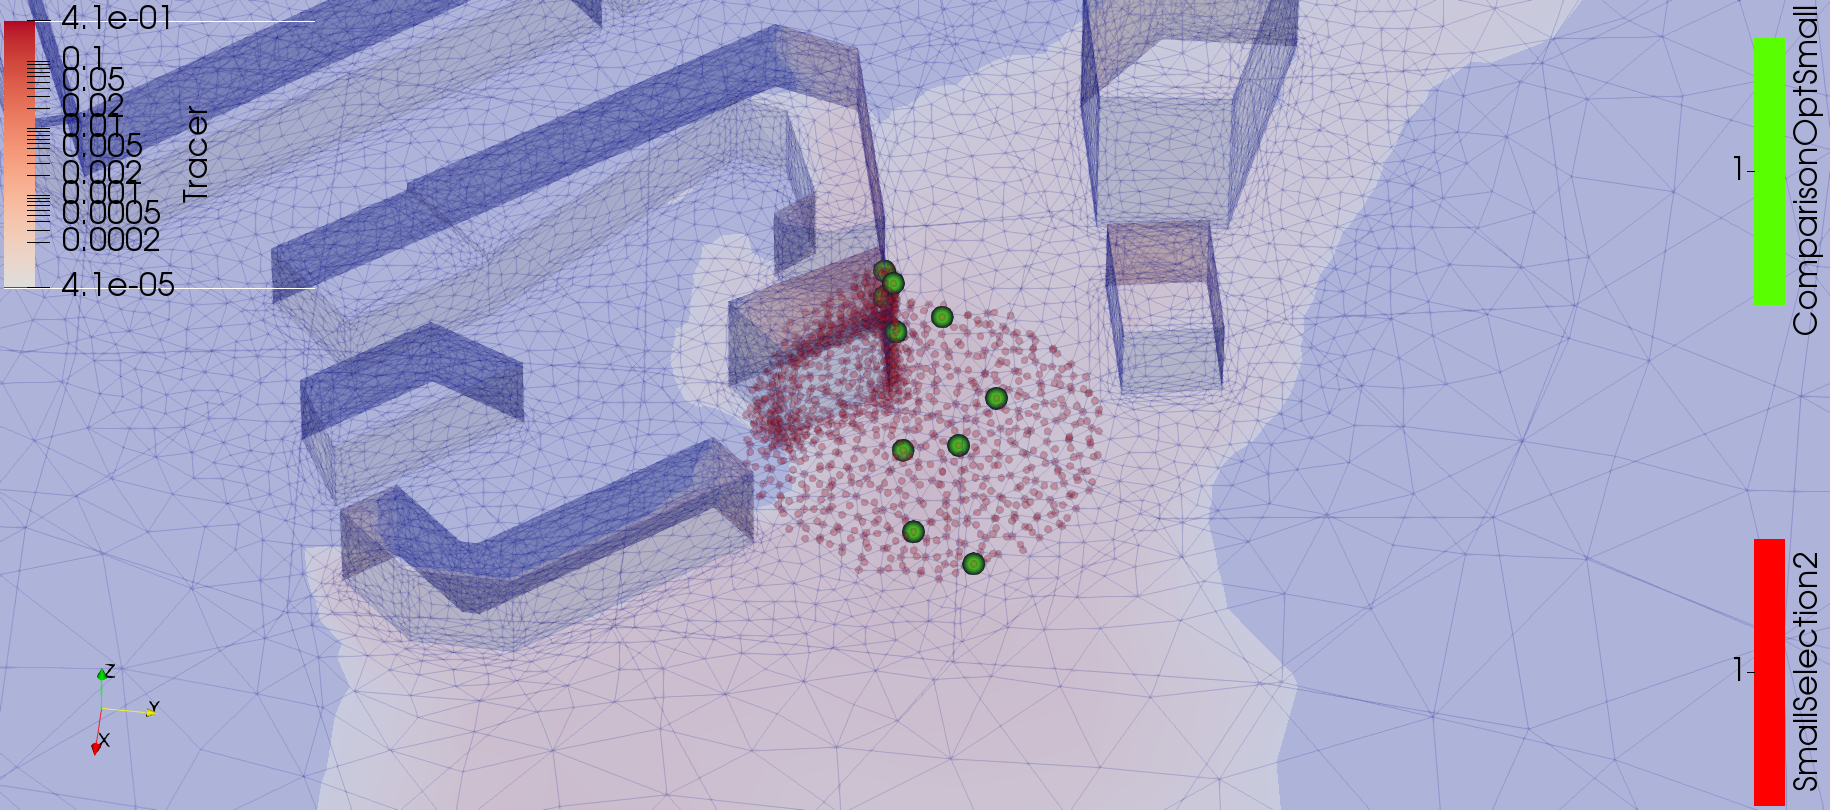
\includegraphics[width=0.8\linewidth]{figures/CompAlg/3rd/non_centered_60.35.0/optimal_screenshot}
    \caption{Optimal Points Location: Illustation}
    \label{fig:opt_small}
\end{figure}

\begin{table}[h]
\centering
\footnotesize
\begin{tabular}{l|rrrrrrrrrr}
\toprule
$\A^*$ &  52731 &  47876 &  3078  &  19782 &  26045 &  30511 &  26754 &  81507 &  11608 &  3903  \\
\midrule
X &  61.31 &  43.55 &  77.31 &  38.75 &  48.23 &  50.48 &  52.36 &  43.10 &  82.40 &  62.01 \\
Y &  40.06 &  27.62 &  35.55 &  35.26 &  29.38 &  30.04 &  44.37 &  27.52 &  44.48 &  32.39 \\
Z &   1.52 &  16.40 &   1.45 &   1.80 &  19.53 &  11.79 &   1.62 &  10.23 &   1.96 &   0.20 \\
\bottomrule
\end{tabular}
\caption{Optimal Points Locations }
\label{tab:opt_small}
\end{table}


We also can plot the Mutual Information Gain $\delta_{y^*}$at each sensor placement on Figure \ref{fig:compAlg:MIGAIN}. What we can see confirms that our Mutual Information is sub-modular, as the Mutual Information Gain is monotonically decreasing. 


\begin{figure}[h!]
\centering
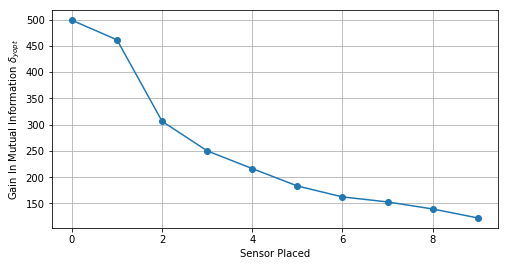
\includegraphics[width=0.6\linewidth]{figures/CompAlg/3rd/non_centered_60.35.0/MIGain}
\caption{Mutual Information Gain for each sensor - Greedy \& Lazy Algorithms}
\label{fig:compAlg:MIGAIN}
\end{figure}


\subsection{Local Kernels Optimisation}

The 3rd Algorithm that we are going to use is the one that is scalable to larger datasets. This scalability is dependent on the parameter $\epsilon$, the thresholding parameter of the covariance. As a consequence the number of selected covariates  $|N(y_{opt},\epsilon)| \leq d $ is fluctuating and influences greatly the speed of the algorithm. It is directly linked to the GP and the size of the covariance matrix to invert.  \\ 

This is why the threshold $\epsilon$ has to be chosen carefully. We are going to show that the speed, the NN distance and the parameter d varies according to $\epsilon$, before choosing a value that will be used for the full-scale optimisation. We compute of a range of values for $\epsilon$ all those results and show them in table \ref{tab:comp:results} and in Figure \ref{fig:comp:results}. \\



\begin{table}[h]
\centering
\scriptsize
\begin{tabular}{l|cccccccccc}
  \toprule
  Threshold $\epsilon$ & $10^{-10} $ &  $10^{-9}$ & $10^{-8}$ & $10^{-7}$ & $10^{-6}$ & $10^{-5}$ & $10^{-4}$ & $10^{-3}$ & $10^{-2}$ & $10^{-1}$ \\
    \midrule
  Distance [m]       &    0.00 &    0.00 &    0.00 &    0.00 &   1.248 &  2.783 & 4.693 & 11.058 & 11.058 & 11.058 \\
Time [s]       & 1660.85 & 1617.92 & 1500.63 & 1151.68 &  520.36 &  60.88 &  2.44 &   1.74 &   3.25 &   2.13 \\
Average d & 1289.40 & 1288.20 & 1284.80 & 1245.60 & 1029.60 & 510.50 & 15.20 &   0.00 &   0.00 &   0.00 \\
  \bottomrule
\end{tabular}
\caption{Local Kernel Results - Tracer}
\label{tab:comp:results}
\end{table}

\begin{figure}[h]
\centering
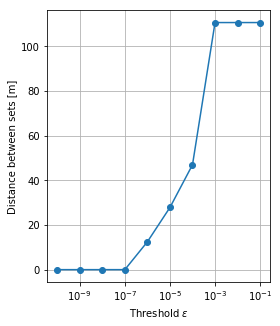
\includegraphics[height=0.33\linewidth]{figures/CompAlg/3rd/non_centered_60.35.0/comp_dist}
~
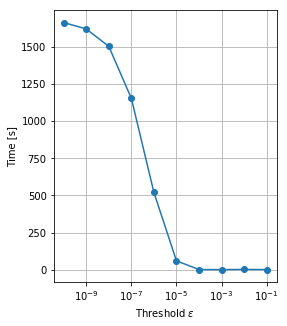
\includegraphics[height=0.33\linewidth]{figures/CompAlg/3rd/non_centered_60.35.0/comp_Time}
~
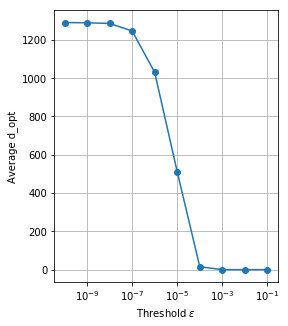
\includegraphics[height=0.33\linewidth]{figures/CompAlg/3rd/non_centered_60.35.0/comp_d_opt}
\caption{Local Kernels: Distance, Time and d, in function of $\epsilon$ - Tracer}
\label{fig:comp:results}
\end{figure}

We see that computation time is correlated with the average number of correlates d. For a threshold bellow $10^{-7}$, we see that the algorithm selects almost every point available and therefore we have computation times of the order of the greedy algorithm. The optimised set of points is then also the same as the greedy and lazy algorithms.\\

By increasing the threshold, we find that the computation time and the number of covariates decrease at the expense of the accuracy represented by the increase in the NN distance between this dataset and the optimal one. We observe also that for $\epsilon > 10^{-3}$, the number of covariates selected d is equal to zero which means that the algorithm updates every position at each iteration and uses for the optimisation only the values of the original covariance, without conditioning them, as the observed set is empty.  \\

Therefore we need to \textbf{fix the threshold} at around $ \epsilon_{opt} = 10^{-6}$, so that the error is still small and the computation time substantially reduced. This threshold will be used on the full-scale optimisation of Tracer Concentration Data.  \\ 


By relocating the centre of the selection sphere, we observe that the optimal threshold is very different from one zone to the other. For example, if we place the subset in a zone where the tracer data is almost always null, we see that the threshold needs to be much smaller to get any results. This is why the value we have chosen was optimised for an area where there is some relevant data. 


\subsection{Approximated Gaussian Processes}

Alternatively, we use the approximation method developed earlier relying on the TSVD of the data, applied to algorithm 2. We proceed to the optimisation of the dataset using different values for the truncation parameter $\tau$. We then plot the computation time and the set distance to the results of the greedy algorithm in function of the truncation parameter in Figure \ref{fig:small_set:tsvd}. \\

\begin{figure}[h]
\centering
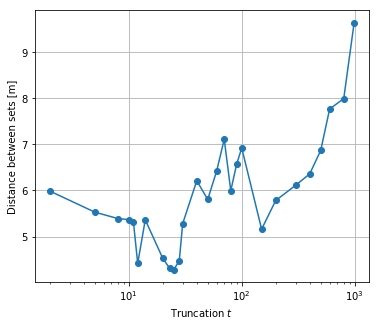
\includegraphics[height=0.33\linewidth]{figures/CompAlg/tsvd/dist_trunc}
~
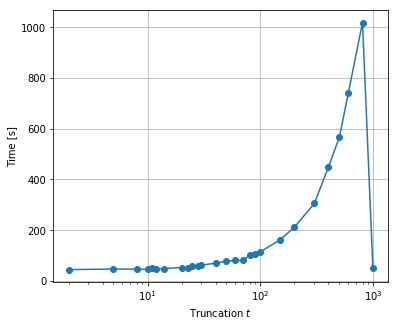
\includegraphics[height=0.33\linewidth]{figures/CompAlg/tsvd/time_trunc}
\caption{TSVD Approximation: Distance and Time in function of $\tau$}
\label{fig:small_set:tsvd}
\end{figure}

As we can see the computation time increases exponentially with $\tau$ and it is then reduced when $\tau$ gets larger than $n=988$.  For the NN distance between those sets and the optimal sets of algorithm 1, we see that it is quite low at the for a small $\tau$, and it reaches a minimum at $\tau_{opt} = 25$. For larger values, the distance is strongly increasing.  We will keep this method and the optimal truncation parameter, for testing on the full dataset in the following section. \\

It is important to mention that the result is here empirical, and that some methods providing optimal parameters are given by \citet{arcucci_optimal_2019}. In this publication, the dataset used is similar and the optimal truncation found is of the same order.  \\

%\subsection{Optimisation on Pressure}
%
%
%
%Now, we are going to compare the performances of the different algorithms using the \textbf{Pressure} Data. 
%
%\subsubsection{Greedy and Lazy Optimisation}
%
%Similarly to the case of \textbf{Tracer}, we consider that the optimal results for this configuration are given by the greedy and lazy algorithms. \\
%
%The optimal set is given in table \ref{tab:opt_small:pressure} and illustrated on Figure \ref{fig:opt_small:pressure}. The points are here too well spread on the optimisation space. They are even situated often near the border of the space. 
%
%
%\begin{figure}[h!]
%\centering
%    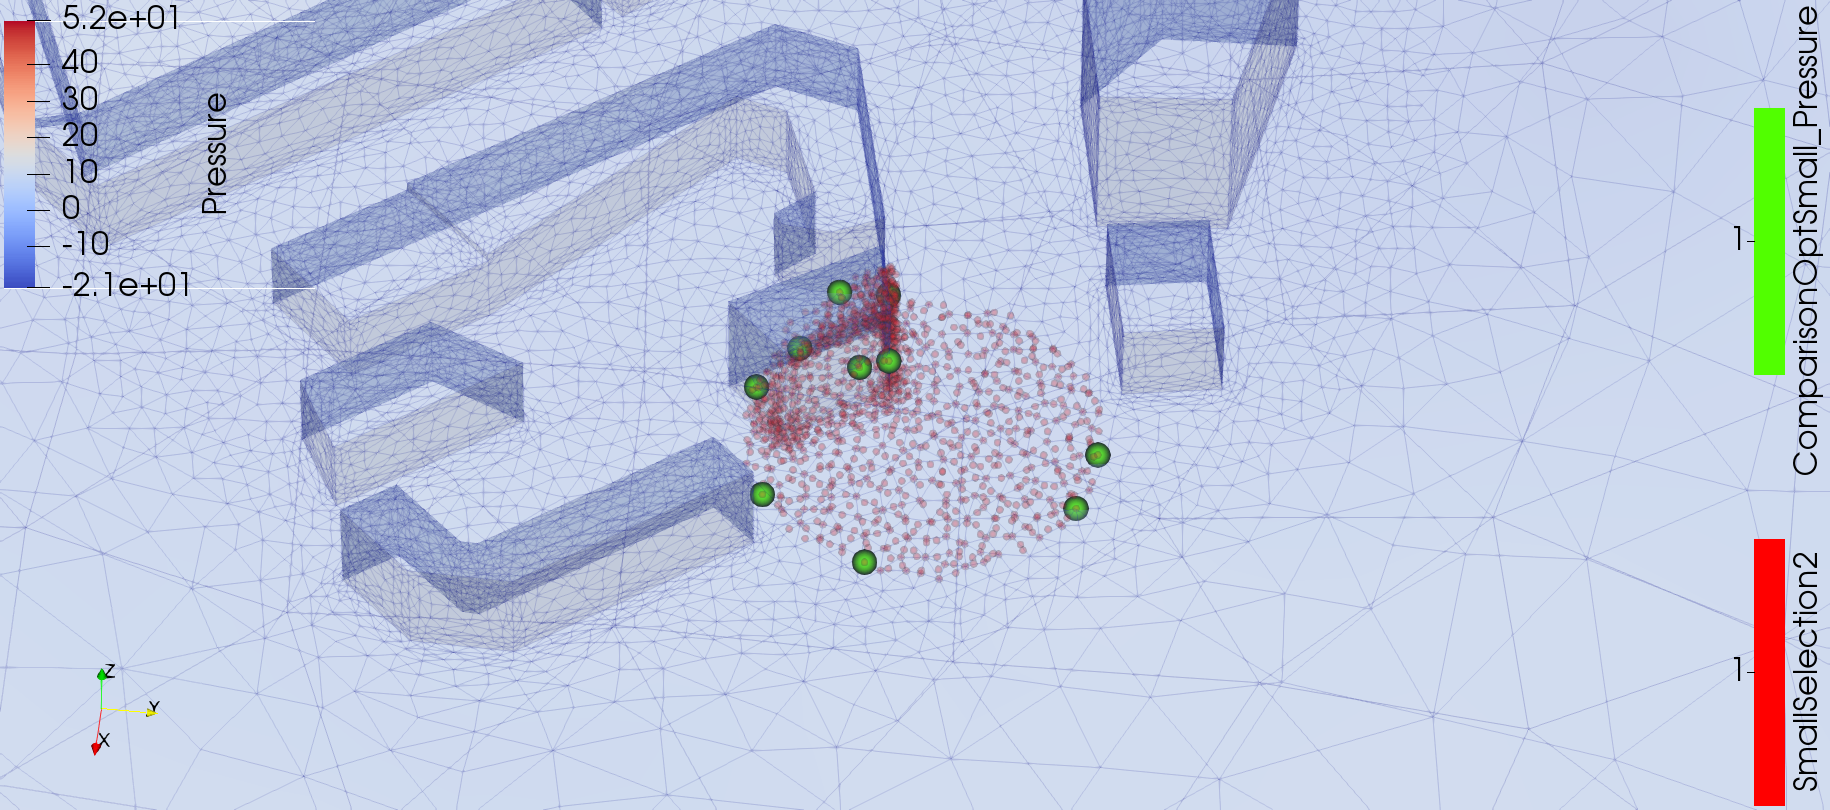
\includegraphics[width=0.8\linewidth]{figures/CompAlg/3rd/pressure_non_centered/optimal_screenshot}
%    \caption{Optimal Points Location: Illustation - Pressure}
%    \label{fig:opt_small:pressure}
%\end{figure}
%
%\begin{table}[h]
%\centering
%\footnotesize
%\begin{tabular}{l|rrrrrrrrrr}
%\toprule
%$\A^*$ &  17899 &  71227 &  71952 &  96870 &  78155 &  28083 &  40511 &  9050  &  74654 &  4146  \\
%\midrule
%X &  47.48 &  54.57 &  49.85 &  73.15 &  40.16 &  57.36 &  69.55 &  83.24 &  52.45 &  60.24 \\
%Y &  16.26 &  25.44 &  22.08 &  14.06 &  27.83 &  11.37 &  57.31 &  29.43 &  29.29 &  59.37 \\
%Z &   2.77 &   8.37 &  18.50 &   1.47 &   7.22 &   5.44 &   0.20 &   1.19 &   7.74 &   0.89 \\
%\bottomrule
%\end{tabular}
%\caption{Optimal Points Locations - Pressure}
%\label{tab:opt_small:pressure}
%\end{table}
%
%\subsubsection{Local Kernels Optimisation}
%
%We also apply the local kernel method to the Pressure Data, and we obtain the results presented in table \ref{tab:comp:results:pressure} and Figure \ref{fig:comp:results:pressure}. The threshold $\epsilon$ varies here between $60$ and $90$, as the threshold value is dependant of the data. \\
%
%We get the same kind of behaviour than in the case of the \textit{Tracer} Data. We choose the optimal threshold $\epsilon^* = 72$. For this value we have a good balance between accuracy and computation time. 
%
%
%
%\begin{table}[h]
%\centering
%\scriptsize
%\begin{tabular}{l|rrrrrrrrrr}
%\toprule
%Threshold $\epsilon$ &     60  &     65  &     70  &    75  &    80  &    82  &    84  &    86  &    88  &    90     \\
%\midrule
%Distance [m]       &    0.00 &    6.62 &   62.98 &  83.54 &  90.57 & 103.48 & 121.92 & 134.86 & 125.57 & 124.73   \\
%Time [s]        & 1217.57 & 1136.29 &  858.54 & 199.86 &  81.43 &  30.06 &  15.18 &   7.95 &   5.47 &   3.89   \\
%Average d & 1289.50 & 1287.30 & 1060.50 & 281.10 & 376.70 & 240.50 & 170.10 &  96.60 &  69.90 &  33.50   \\
%\bottomrule
%\end{tabular}
%\caption{Local Kernel Results - Pressure}
%\label{tab:comp:results:pressure}
%\end{table}
%
%\begin{figure}[h]
%\centering
%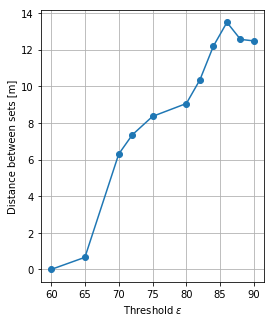
\includegraphics[height=0.33\linewidth]{figures/CompAlg/3rd/pressure_non_centered/comp_dist}
%~
%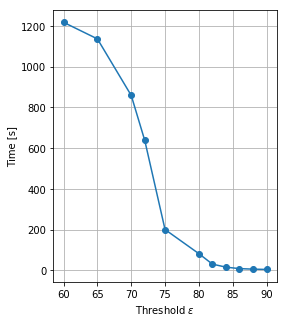
\includegraphics[height=0.33\linewidth]{figures/CompAlg/3rd/pressure_non_centered/comp_Time}
%~
%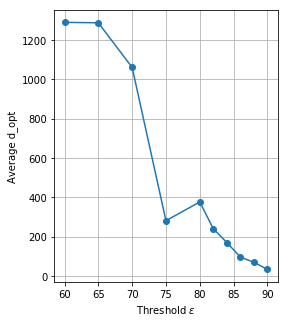
\includegraphics[height=0.33\linewidth]{figures/CompAlg/3rd/pressure_non_centered/comp_d_opt}
%\caption{Local Kernels: Distance, Time and d, in function of $\epsilon$ - Pressure}
%\label{fig:comp:results:pressure}
%\end{figure}
%
%
%
%
%
%\subsubsection{Approximated Gaussian Processes}
%
%Here we apply also the method based on TSVD, which reduces the dimension of the data to compute an approximate GP. In the Figure \ref{fig:small_set:tsvd:pressure}, we plot in function of the truncation parameter the the distance between the set and the optimal set found by algorithm 1.
%
%
%
%\begin{figure}[h]
%\centering
%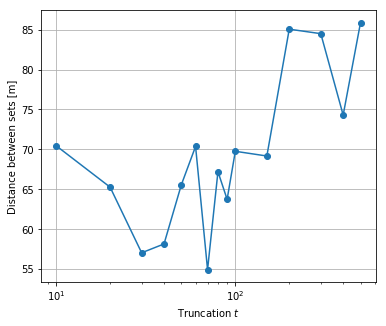
\includegraphics[height=0.33\linewidth]{figures/CompAlg/tsvd/dist_trunc_pressure}
%~
%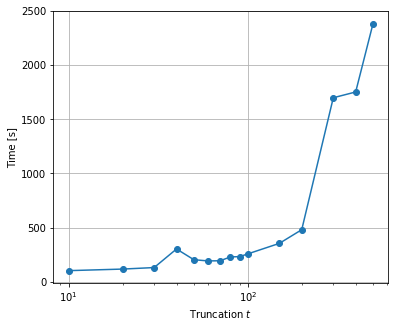
\includegraphics[height=0.33\linewidth]{figures/CompAlg/tsvd/time_trunc_pressure}
%\caption{TSVD Approximation: Distance and Time in function of $\tau$ - Pressure}
%\label{fig:small_set:tsvd:pressure}
%\end{figure}
%
%We have similar results compared to the \textit{Tracer} field. We choose a truncation parameter $\tau=25$, which has a good balance between computation time and accuracy. 

%%%%%%%%% OPTIMISATION %%%%%%%%

\section{Full Scale Optimisation Results}

After the analysis of different algorithm results on a smaller dataset, we are now going to use the most scalable algorithms with the appropriate parameters on the full dataset. The set of points used is the preselected dataset containing $23'643$ locations. \\

In this section, we will present the results of two optimisations, compare them in term of computation speed and proximity. 


%\subsection{Optimisation on Tracer Concentration}


\subsection{Local Kernel Algorithm} \label{sec:res:localK}

We first use the Local Kernel Algorithm \ref{alg:local}. The covariance between the points is computed using the OAS estimator. \\


For this experiment we used the previously defined value of threshold: $\epsilon = 10^{-6}$. Such that the number of points highly correlated to the last positioned sensor is $|N(y_{opt},\epsilon)| \leq d $. \\ 

The algorithm computes the following results in $23797.2$ seconds or $6.61$ hours. \\

We are computing for each iteration the size of this set. This number is directly linked to the size of the covariance matrix being inverted in the GPs. As we are placing 10 sensors, we have 10 values of this quantity that is computed at each iteration of the main loop. Results can be found in table \ref{tab:full:d_opt}. The average value is $4'374.7$. This shows that indeed the optimisation problem is solved in a reduced time as it doesn't use all the $23'643$ locations of our dataset, but $18.50$\% of it.   \\

\begin{table}[h]
    \centering
    \begin{tabular}{l|cccccccccc}
    \toprule
    Sensor & 1 & 2 & 3 & 4 & 5 & 6 & 7 & 8 & 9 & 10 \\     \midrule
        $|N(y_{opt},\epsilon)|$ & 4338 & 4938 & 5066 & 5362 & 4239 & 4164 & 3377 & 4632 & 3511 & 4120 \\     \bottomrule

    \end{tabular}
    \caption{Number of highly correlated points at each iteration}
    \label{tab:full:d_opt}
\end{table}


We visualise the position of the optimal set of sensor points $\A^*$ at different scales in Figure \ref{fig:full_set:position:zoom}. The coordinates of the points are expressed in the table \ref{tab:full:data}. \\


\begin{table}[h]
\centering
\footnotesize
\begin{tabular}{l|rrrrrrrrrr}
\toprule
$\A^*$ &  56588 &  52731 &  73959 &  43278 &  3078  &  19782 &  56257 &  55640 &  10357 &  54786 \\ \midrule
X &  41.61 &  61.31 &  30.32 &  22.79 &  77.31 &  38.75 &  91.19 &  50.10 &  62.13 &   1.62 \\
Y &  27.21 &  40.06 &  26.06 &  25.81 &  35.55 &  35.26 &  35.16 &  29.00 &  45.23 &  19.99 \\
Z &  16.73 &   1.52 &  11.19 &  11.79 &   1.45 &   1.80 &   1.82 &  16.41 &   1.64 &  13.81 \\
\bottomrule
\end{tabular}
\caption{Optimal Points Locations - Tracer}
\label{tab:full:data}
\end{table}



\begin{figure}[h!]
\centering
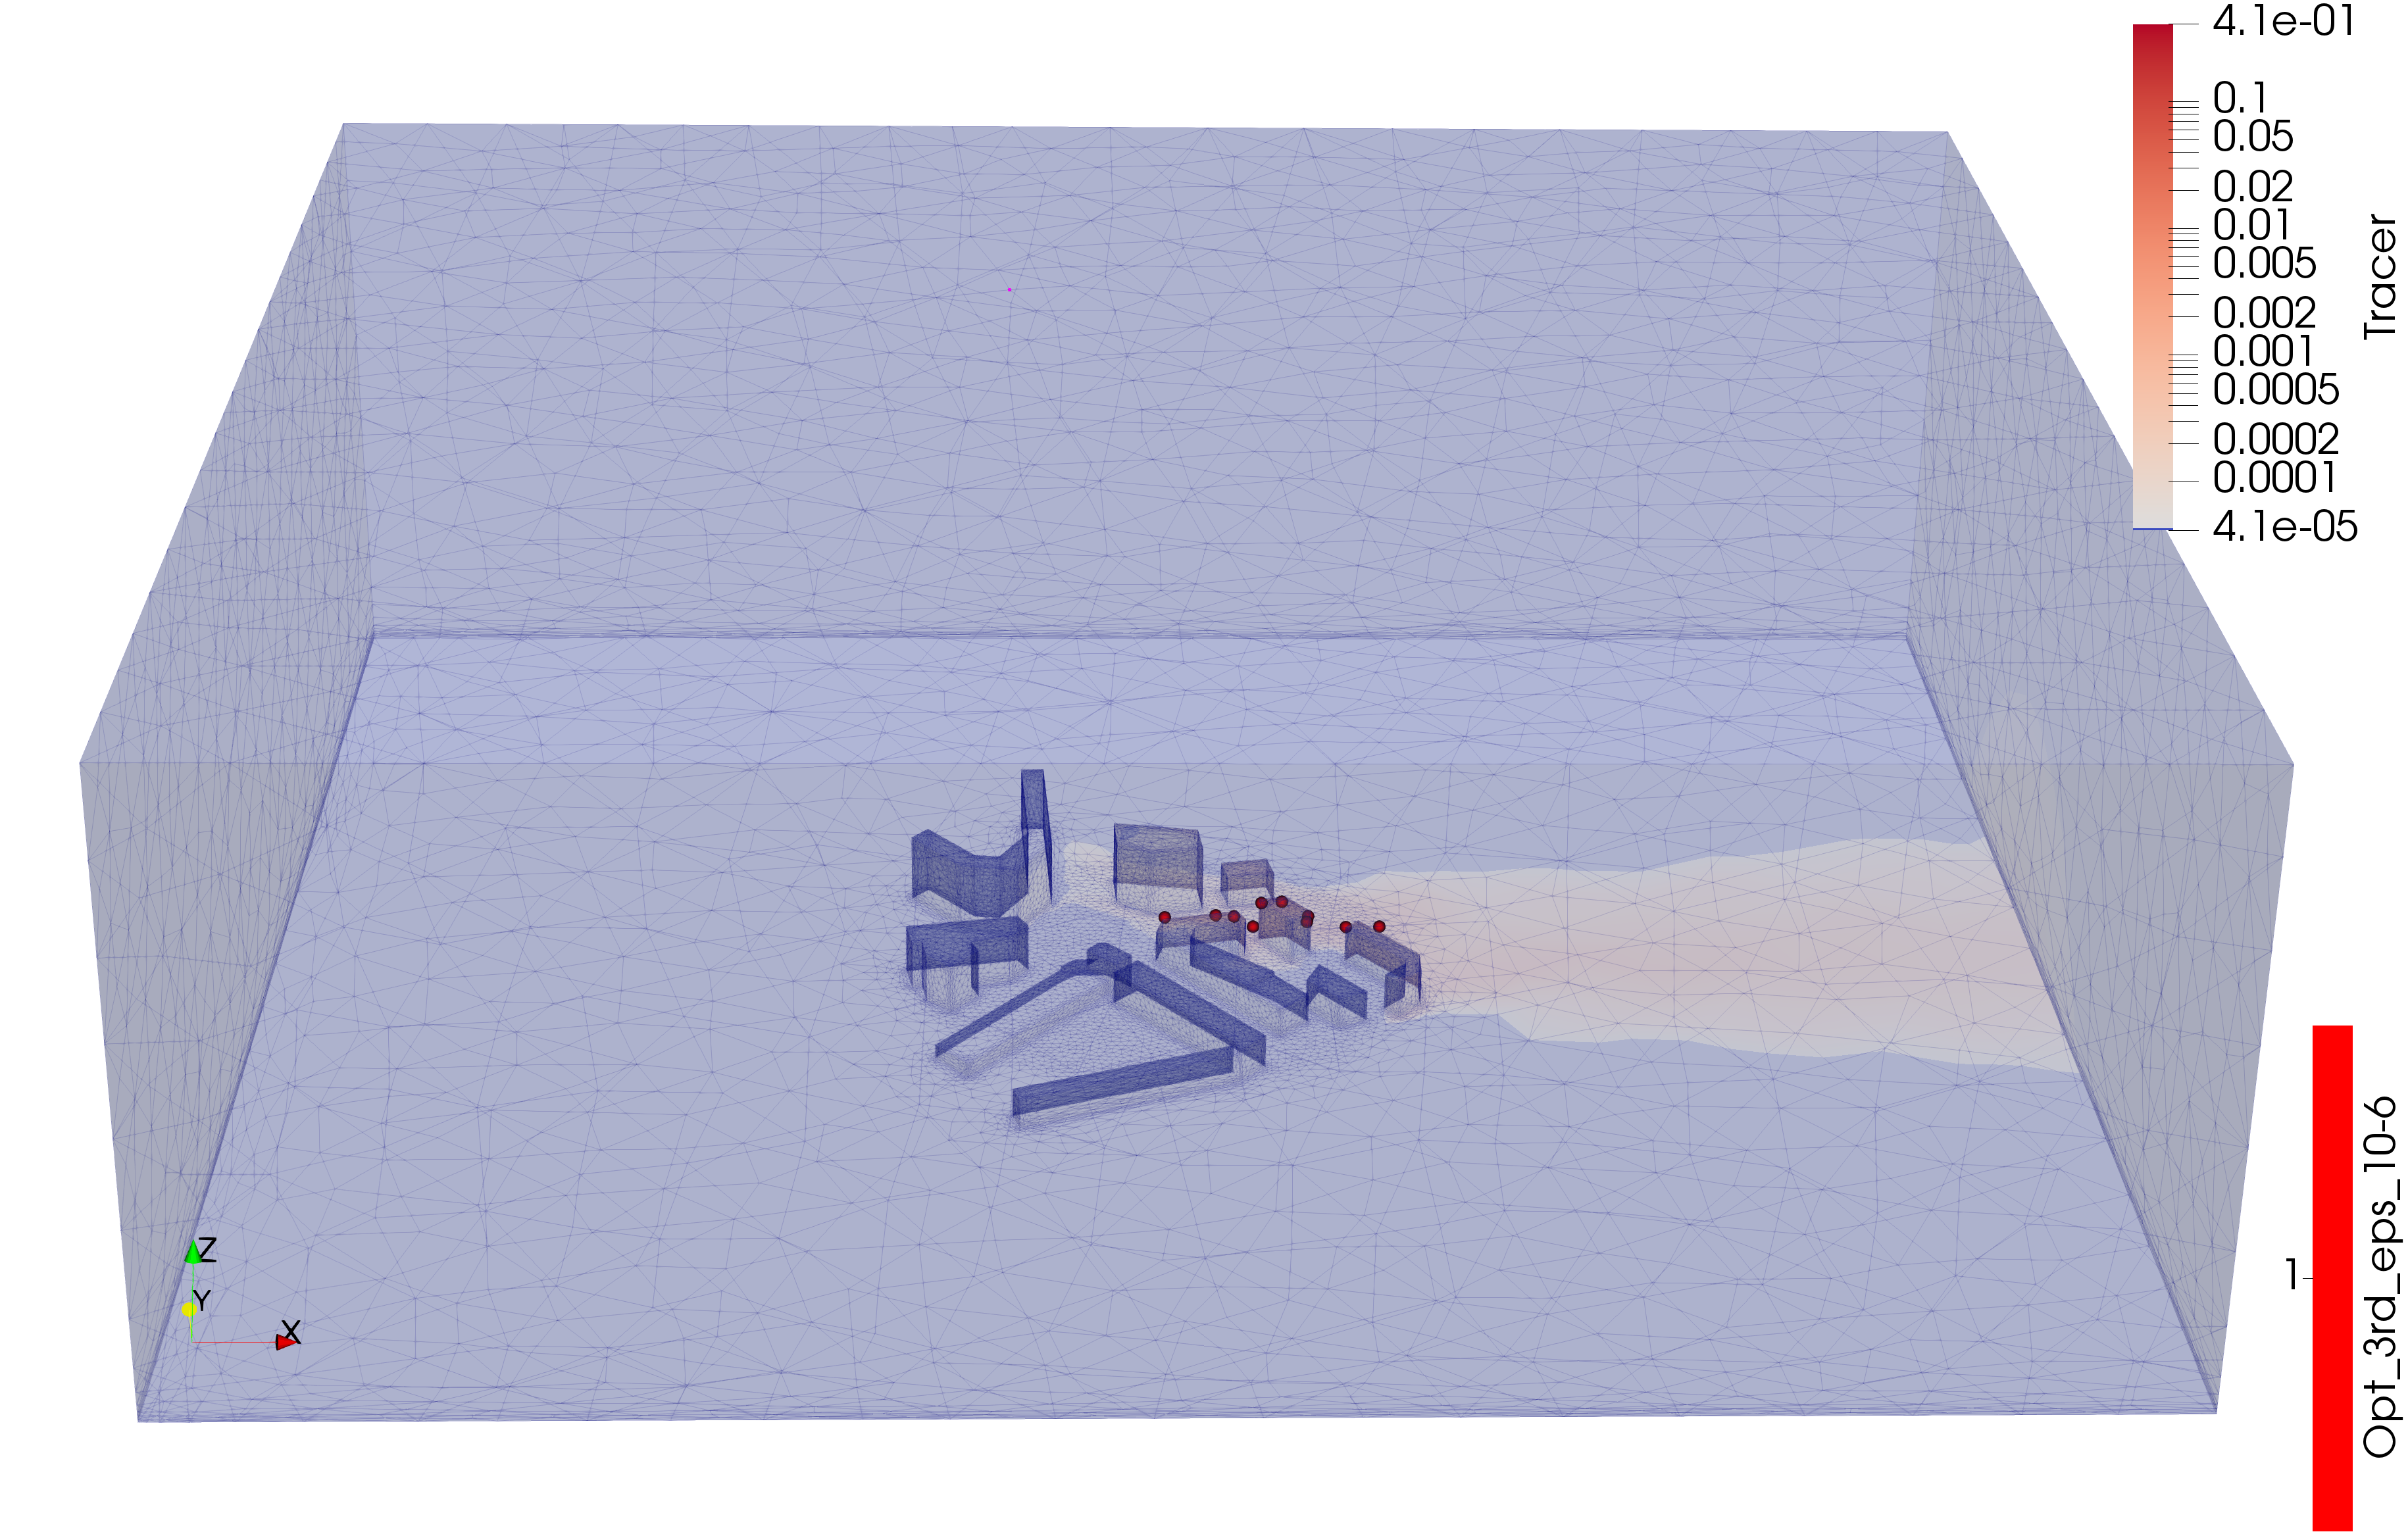
\includegraphics[width=0.7\linewidth]{figures/MainOptimResults/alg3opteps10-6_sideall_screenshot}
\smallbreak
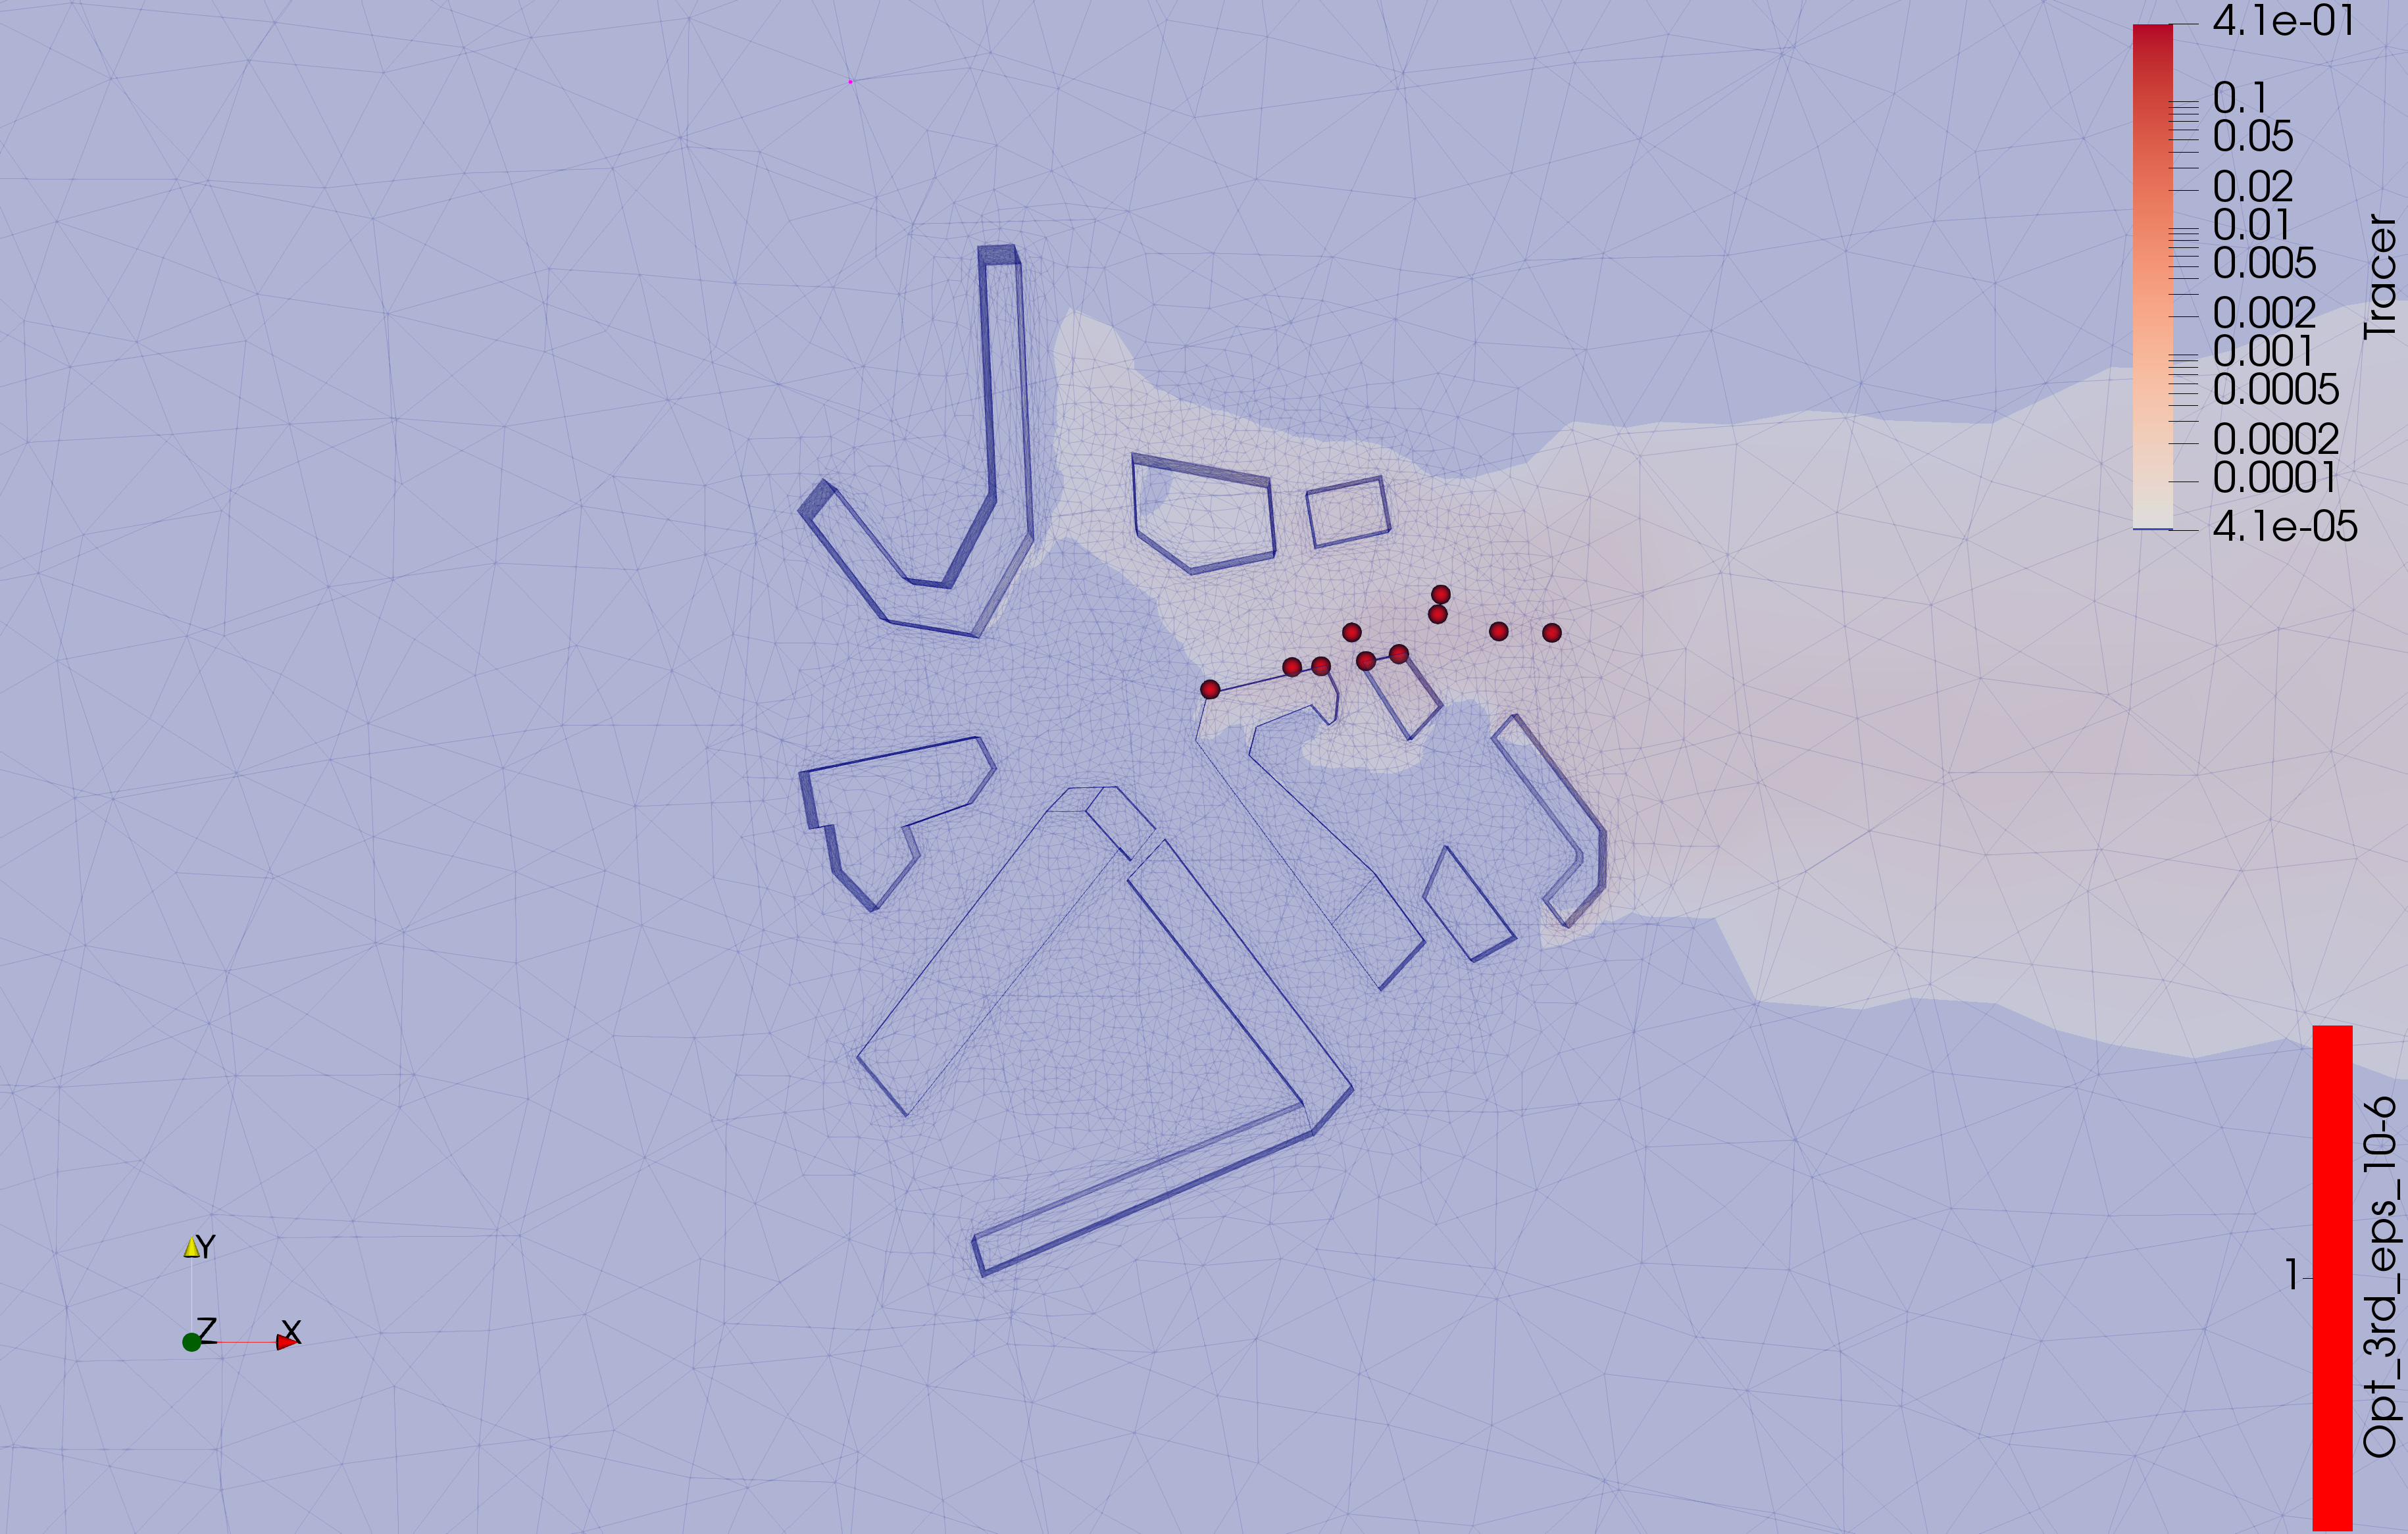
\includegraphics[width=0.7\linewidth]{figures/MainOptimResults/alg3opteps10-6_top_screenshot}
\smallbreak
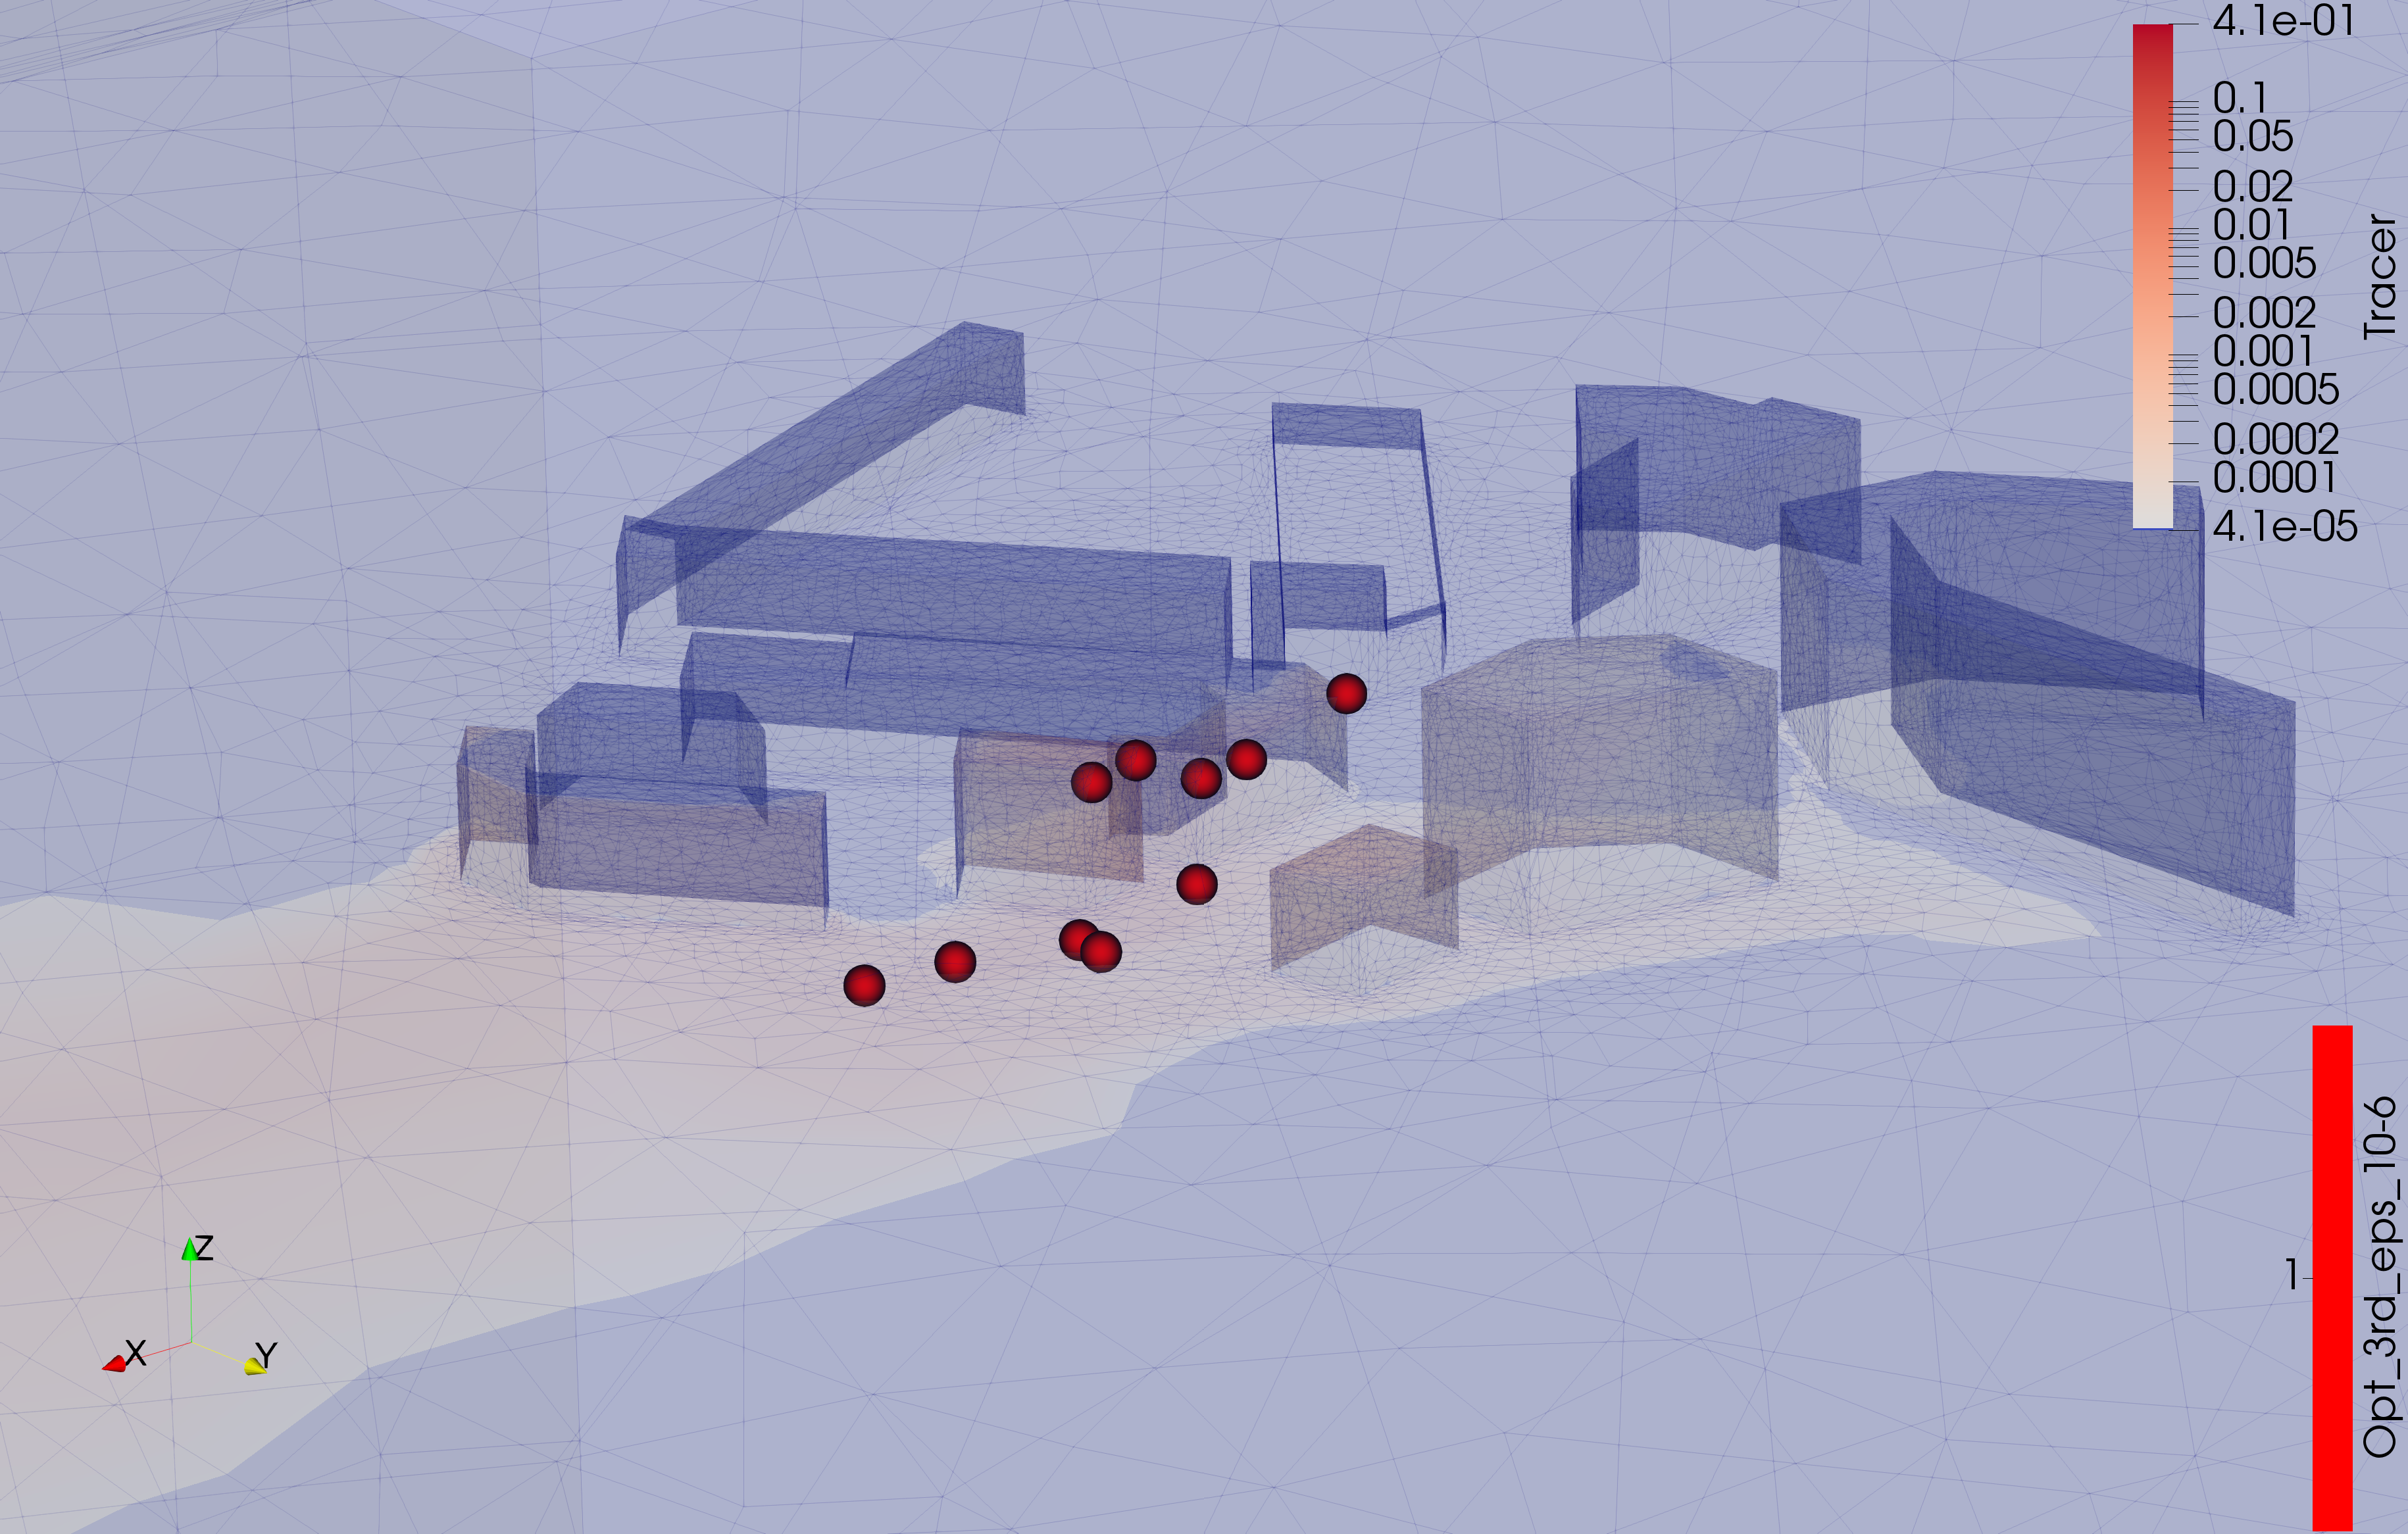
\includegraphics[width=0.7\linewidth]{figures/MainOptimResults/alg3opteps10-6_zoom_screenshot}
\caption{Position of the Optimal Set}
\label{fig:full_set:position:zoom}
\end{figure}


\paragraph{Description}

The location of our optimal set of points is split between points situated on the buildings (5 points) and around the ground level (5 points). They are situated in the middle of the tracer concentration beam and are close to the centre of the domain where the mesh density is maximal. \\ 

The points are roughly aligned in the wind direction, which is a good thing because the tracer is propagating itself from the centre of the domain, pushed by the wind in the east direction. Points along this direction are less correlated with each other than points perpendicular to this direction, as the tracer reaches them at the same time. Therefore it makes sense that the selected points are roughly along the wind direction as it will maximise the information retrieved during the propagation of the tracer. \\

Finally we observe the Mutual information gain $\delta_{y^*}$ for each placed sensor on Figure \ref{fig:full_set_Alg3:MIGAIN}. It confirms that our MI is sub-modular as here again the decreasing of the MI difference is monotonic. 
 \\


\begin{figure}[h]
\centering
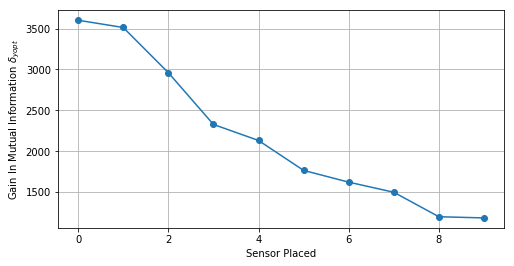
\includegraphics[width=0.6\linewidth]{figures/MainOptimResults/alg3opteps10-6_DeltaY}
\caption{Mutual Information Gain for each sensor - Algorithm 3}
\label{fig:full_set_Alg3:MIGAIN}
\end{figure}




\subsection{Lazy Algorithm with TSVD} \label{sec:res:TSVD}

We apply on the same dataset the 2nd Algorithm with the approximated GP that we defined earlier. We use the truncation parameter $\tau_{opt} = 25$. The results we obtain are displayed in table \ref{tab:tsvd:data} and Figure \ref{fig:full_set_tsvd:position:zoom}, along with the previous optimal results. \\ 
 
This algorithm computes the following results in $18083.87$ seconds or $5.02$ hours. 
 
 \paragraph{Description}

Here again, the location of our optimal set of points is split between points situated on the buildings (3 points) and around the ground level (7 points). The locations are more spread than the other set of points. Two locations are even at the border of the candidate dataset. The NN distance between this set and the previous one is $13.84$m,  which is not very important with regards to the size of the space.  \\ 




\begin{table}[h]
\centering
\footnotesize
\begin{tabular}{l|rrrrrrrrrr}
\toprule
$\A^*$ &  38726 &  14276 &  91348 &  5338  &  40994 &  29626 &  65851 &  65734 &  851   &  2293  \\
\midrule
X & -50.50 &  35.63 &  43.05 & 137.58 &  80.34 &  27.79 &  49.54 &  54.59 &  77.54 &  62.03 \\
Y &  48.85 &  58.69 &  27.51 &  55.78 &  76.20 &  26.24 &  28.88 &  25.42 &  34.82 &  41.92 \\
Z &  14.84 &   0.20 &   7.76 &   0.20 &   0.20 &  12.06 &  17.65 &   3.80 &   0.20 &   0.20 \\
\bottomrule
\end{tabular}
\caption{Optimal Points Locations TSVD - Tracer}
\label{tab:tsvd:data}
\end{table}


\begin{figure}[h!]
\centering
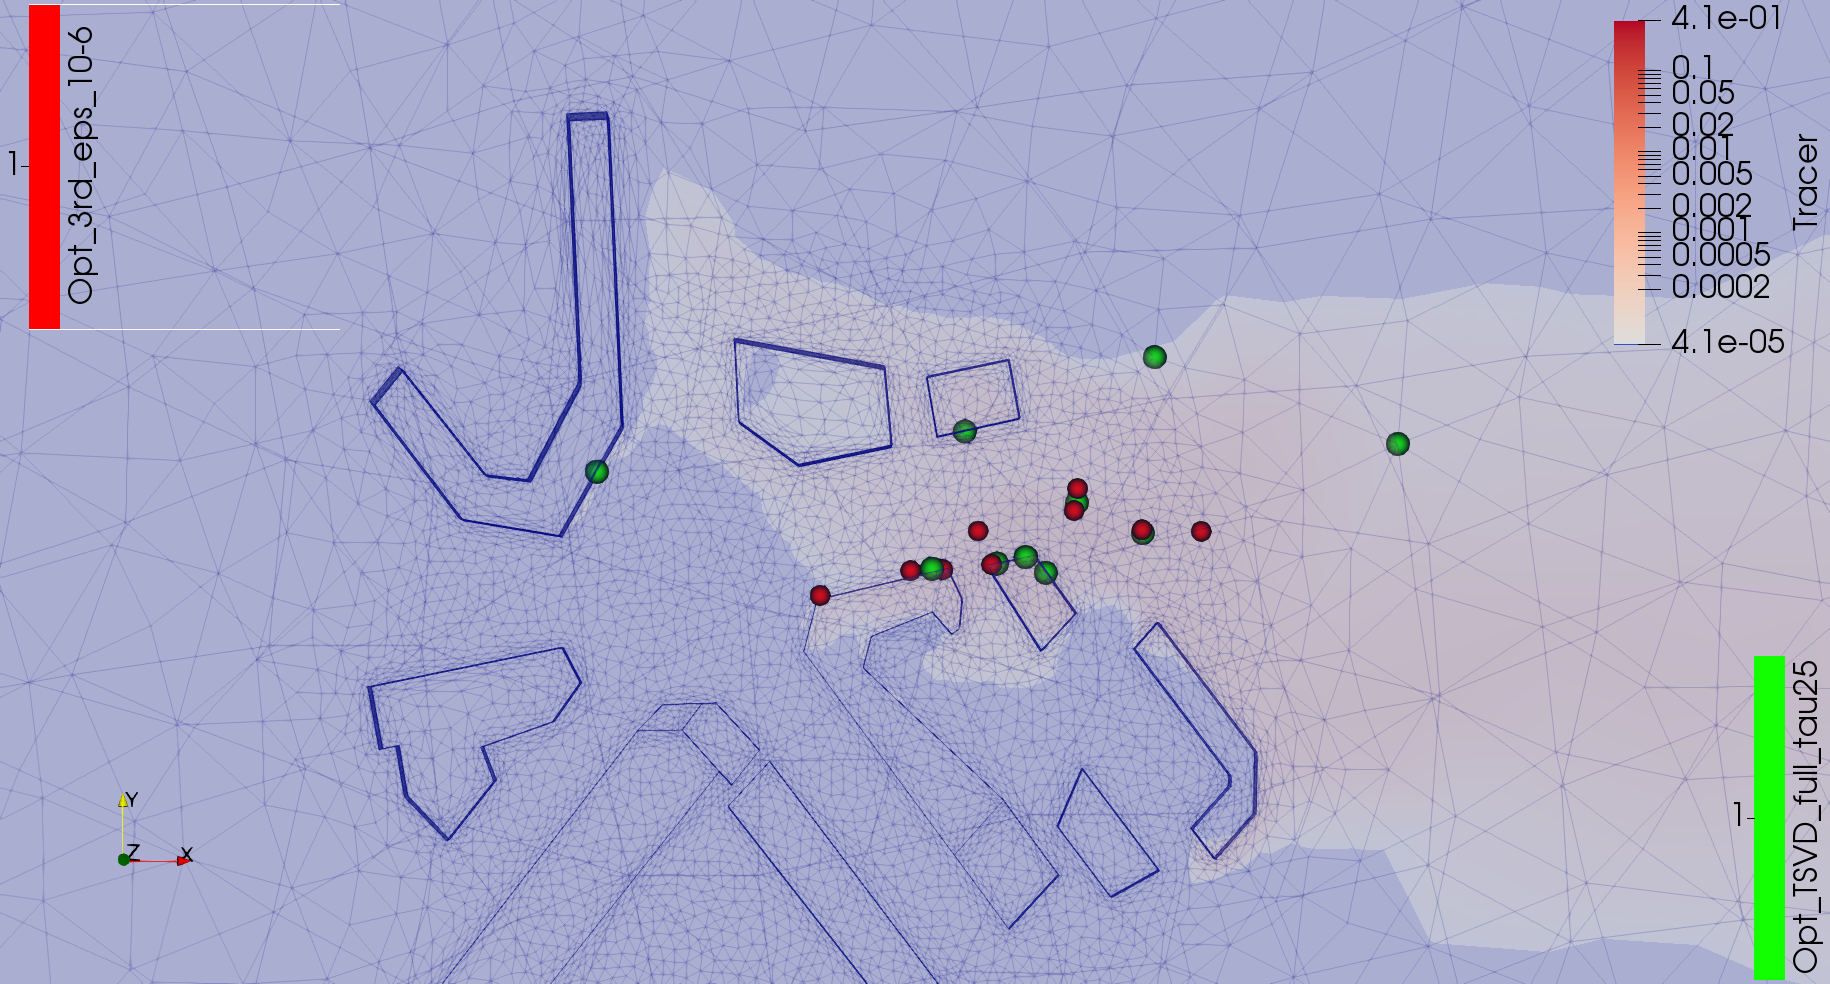
\includegraphics[width=0.7\linewidth]{figures/MainOptimTSVD/tsvd+3rd_position_top}
\smallbreak
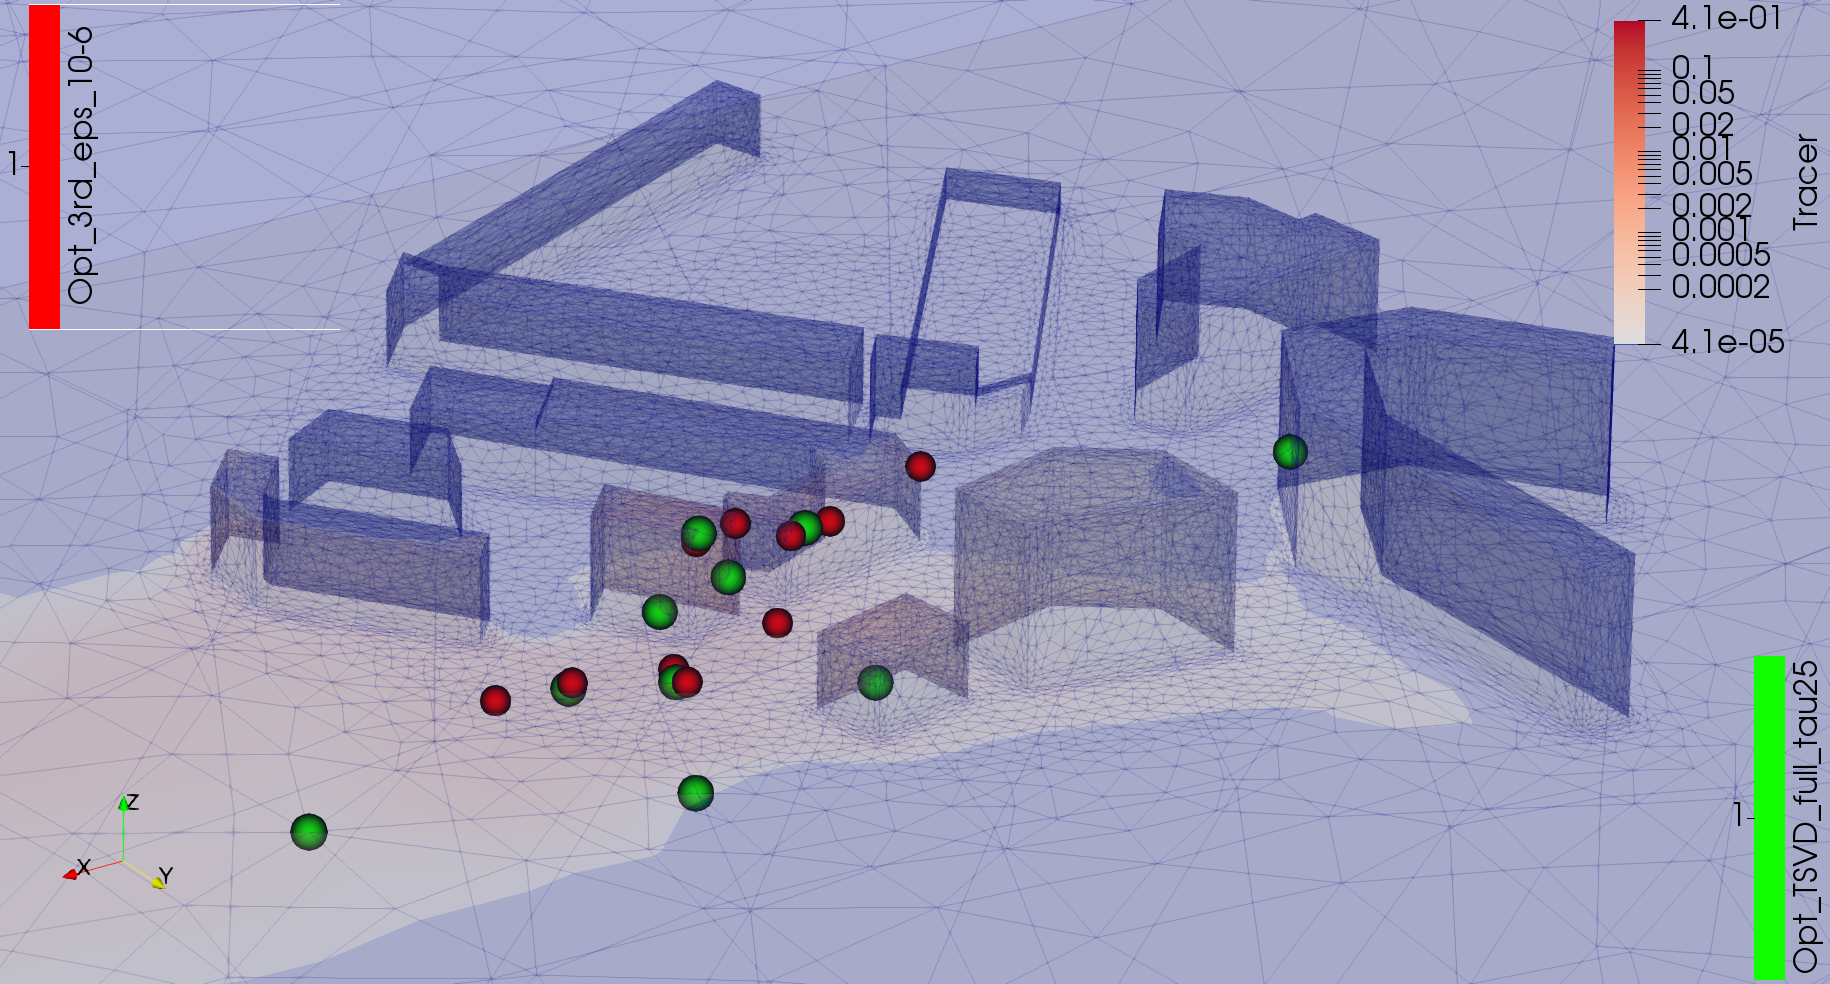
\includegraphics[width=0.7\linewidth]{figures/MainOptimTSVD/tsvd+3rd_position_side}
\caption{Position of the Optimal Set: Main View $\tau = 25$}
\label{fig:full_set_tsvd:position:zoom}
\end{figure}


Finally we observe the Mutual information gain $\delta_{y^*}$ for each placed sensor on Figure \ref{fig:full_set_tsvd:MIGAIN} is also constantly decreasing. However we can observe that it is not linear, as it was in the small set experimentation and in the Algorithm 3 optimisation. 
\\

\begin{figure}[h!]
\centering
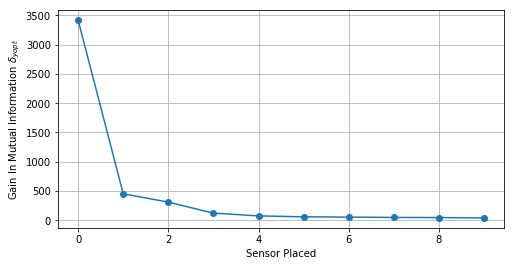
\includegraphics[width=0.6\linewidth]{figures/MainOptimTSVD/MIGain}
\caption{Mutual Information difference for each sensor - TSVD}
\label{fig:full_set_tsvd:MIGAIN}
\end{figure}




%
%\subsection{Optimisation on Pressure}
%
%
%
%\begin{table}[h]
%\centering
%\footnotesize
%    \begin{tabular}{l|rrrrrrrrrr}
%\toprule
%$\A^*$ &  72496 &  75832 &  85761 &  86497 &  26107 &  17851 &  36552 &  38178 &  3351  &  36551 \\
%\midrule
%X & -54.41 & -46.24 & -51.00 & -42.50 & -52.34 & -50.68 & -49.55 & -48.37 & -52.88 & -54.55 \\
%Y &  70.39 &  95.22 &  72.66 & 132.29 &  31.07 &  31.96 &  32.72 &  33.31 &  28.94 &  26.82 \\
%Z &   8.70 &   3.28 &  29.14 &   1.37 &   1.16 &   0.20 &   1.44 &   0.80 &   0.20 &   0.20 \\
%\bottomrule
%\end{tabular}
%\caption{\caption{Optimal Points Locations - Pressure}
%\end{table}
%
%\todo{Fill Pressure Data Optimisation}



%%%%%%%%% OPTIMISATION %%%%%%%%

\section{Application to Variational DA}


As we have seen, one way of applying the results to a real situation is to proceed to a Variational Data Assimilation of the points selected. By taking results of a simulation and applying DA on our selected points we can try to see if the results are usable in the context of the MAGIC project. 

\subsection{Parameters of the Experiment} 

For this experiment, we chose to consider the same simulation data than previously: the 3D smallLSBU.  We choose as the observation state, the step $988$ of the simulation, and as background state, the step $100$ of the simulation. \\

We compute the Variational DA on the 10 optimal points selected by the algorithms and compute the background error and the error after the DA procedure.  
%\subsection{VarDA on Tracer Concentration}
%
%First we apply our DA algorithm on the \textit{Tracer} Data. 

\subsection{VarDA on Local Kernel Results}

First, we run the VarDa Algorithm and obtain the following. 
\begin{table}[h]
\centering
    \begin{tabular}{c|c|c}
    \toprule
          MSE [xDA] & MSE [xB] &  Imp. [xDA / xB] \\ \midrule
         $7.7375 \cdot 10^{-17}$ &  $0.9923$ & $7.7975 \cdot 10^{-17}$ \\ \bottomrule
    \end{tabular}
    \caption{VarDA on Local Kernel Results. }
\end{table}

\paragraph{Comparison to Random}

To compare those results to another set of points, we proceed as follows. Around every single point of $\A^*$, we select randomly (uniformly) a point located within a radius of $R=10m$. This allows us to compare the results to some random set that is close to the optimum. We then proceed to $1'000$ different random selection and compute the average errors and their standard deviations, stated in table \ref{tab:varDa:random}. \\


\begin{table}[h]
\centering
\begin{tabular}{l|cc}
\toprule
               & Average & Std Dev \\ \midrule
MSE [xDA]      & $6.1008 \cdot 10^{-17}$  & $4.1680 \cdot 10^{-17}$  \\
MSE [xB]       & $0.6538$  & $0.1718$  \\
Imp. Ratio [xDA / xB]  &   $9.3313 \cdot 10^{-17}$  & - \\ \bottomrule
\end{tabular}
    \caption{VarDA on $1'000$ Near Random Points: Local Kernel Results}
    \label{tab:varDa:random}
\end{table}

\paragraph{Analysis}

We can see that the error of the optimal set $\A^*$ is very small on the DA results, almost negligible. The improvement form the pre-assimilation background error is of almost $100\%$. This shows that this set of points has some good properties for Data Assimilation. \\

By comparing those results to the $1'000$ random samples, we see that the average is very close to the error of the optimal set. However, the improvement from the background error is smaller for the random sets. In this way, we have better results for the optimal set of points.  



\subsection{VarDA on Gaussian Approximation Results}

We then run the same algorithm on the optimal set found with the lazy algorithm combined with TSVD GP approximation. 

\begin{table}[h]
\centering
    \begin{tabular}{c|c|c}
    \toprule
          MSE [xDA] & MSE [xB] &  Imp. Ratio [xDA / xB] \\ \midrule
        $9.8945 \cdot 10^{-17}$  &  $1.1354$ & $8.7145 \cdot 10^{-17} $ \\ \bottomrule
    \end{tabular}
    \caption{VarDA on TSVD Results. }
\end{table}

\paragraph{Comparison to Random}

To compare those results to another set of points we proceed as previously. The results for $1'000$ random sets sampled at a $10$m radius from each optimal points are given in table \ref{tab:TSVD:random}. 
 \\


\begin{table}[h]
\centering
\begin{tabular}{l|cc}
\toprule
               & Average & Std Dev \\ \midrule
MSE [xDA]       & $6.6843 \cdot 10^{-17}$  & $4.9458 \cdot 10^{-17}$  \\
MSE [xB]  & $0.6725$  & $0.2148$  \\
Improvement Ratio  [xDA / xB]  & $9.9381 \cdot 10^{-17}$  & - \\ \bottomrule
\end{tabular}
    \caption{VarDA on 500 Random Points: TSVD Results}
    \label{tab:TSVD:random}
\end{table}

\paragraph{Analysis}

We observe the same phenomenon than with the \textit{Tracer} Local Kernel results. The DA error is negligible and the Improvement is better with our optimal points. 


%\subsection{VarDA on Pressure}
%
%Now we apply the DA procedure to the \textit{Pressure} Data. 
%
%\subsubsection{VarDA on Local Kernel Results}
%
%\subsubsection{VarDA on Gaussian Approximation Results}
%




\subsection{Limitations of the Application}

Even if the error magnitude is not decreasing, we can see an improvement in the value of the computed ratio between the DA error and the background error. It has been shown by \citet{arcucci_optimal_2019}, that when the simulation is continued after DA, the an initial improvement is propagated and an initial better improvement leads to better results overall for both the sensors and un-monitored spaces. 

%As we have seen the results given by this simple VarDA application are not very satisfying. We observe clearly that the randomly selected points give results \textbf{as good as} the optimal points. \\

We are here measuring the error directly after the assimilation and only on the 10 assimilated points. As VarDA is an optimisation problem that minimises this error,  considering the small number of points and the fact that there is no dimensionality reduction of the deviation matrix, it is quite natural that this error is negligible.  \\

To draw more conclusions on the validity of our set of points, we would need to continue the simulation after the DA procedure and compare after some time the states of all the points of the space with different assimilated sets of points. \\



% Furthermore, we have to consider the DA as a simple application of our near-optimal sensor positioning algorithm. We have not proven any link between the Mutual Information criterion, that we had optimised to find the optimal points, and the optimality of the DA procedure. \\
 
% Not taking into account the dynamics of the space. Assumption of samples are independent and identically distributed and samples of the sample Gaussian probability distribution. 

% We have to keep in mind the DA Algorithm used is computing the MSE only on the 10 points of interest. We do not study here the propagation after the DA, so we are not able to see the impact of our selected set on the rest of the locations of the space. \\




%% TEMP %%% CHAPTER: progress
%%%%%%%%%%%%%%%%%%%%%%%%%%%%%%%%%%%%
\chapter{Progress}

This chapter exposes the work done until now in the project. It will focus on the choices I have made, the stages of developpment and the questions remaining. All the codes are available on the Github repository of the project.


\section{Data Exploration}

As the main dataset, we use the simulation results on an unstructured mesh of measurements with a very high density in the low middle part of the space. The simulation used has $100'040$ points over $988$ timestamps. For the purpose of testing our codes and algorithms,  we are going to use subset of the whole dataset containing a few hundreds to a few thousands of points. I have made the choice to first use a subset of the whole dataset containing $2'488$ point and created by cropping the space to a cube of $30\times30\times30\times$ at the center of the original space. 


 Several fields are present in the simulation : the \textbf{pressure}, the \textbf{tracer} concentration, the \textbf{background tracer} concentration and the \textbf{velocity}. We represent in the next figures, two cuts made to visualise the tracer and the tracer background. \\ 

The \textbf{tracer} represents the propagation of a pollutant generated from the centre of the domain at ground level. It aims a representing a busy intersection. \\

The \textbf{background tracer} represents pollution waves common in urban environment. Its characteristic generation equation is periodic and given by : 

\begin{equation}
	C(t)= \frac{1}{2} \left( \sin \left( \frac{2\pi t}{T} \right) + 1 \right)
\end{equation}



As we can see by observing the time propagation of those fields,  the wind is pushing the pollutants in a certain direction. Because of this, be observe that the \textbf{tracer} concentration is mainly visible downwind, in contrast of the \textbf{background tracer} which has visible propagation over the whole space. We can therefore already deduce that the \textbf{background tracer} contains much more information and should be used for optimising the sensor positions. 


\section{Implementation}

In this section I will quickly review the functionalities that I have implemented and that are working to this day. I relied on Python 3.7, various libraries that I ran my code on the cluster of the DSI.  \\

\subsection{Initialisation}
The raw data is contained in VTK files. I have implemented functions in python that allows the importation, the cropping of the space, the extraction of the fields and interest and the location of the points and the saving in files for making quicker the loading procedure. 

\subsection{Modeling}

I have implemented the full GP training and estimation directly using numpy. It this implementation I have chosen to use a kernel with arbitrary parameters in order to test the accuracy of the optimisation. \\

After this I have used the GPy library \citep{gpy_gpy:_2014} for its full GP implementation and its hyper-parameters optimisation functionalities. The kernel parameters here were optimised using the integrated methods and the model was trained on the full subset of data. \\

I have also implemented using GPy library a spare GP modelisation. GPy includes an optimised implementation of the \textbf{VFE} sparse GP. It enables the optimisation of the variational parameters and the hyper-parameters such as the position of the inducing points. 

\subsection{Optimisation}

I have used the previously trained GPs models in the algorithms described earlier. I have implemented in python two of the proposed optimisation algorithms. The naive greedy approach (algorithm \ref{alg:greedy} ). \\
The Lazy approach developed using python heaps. (algorithm \ref{alg:lazy}). This version is as expected much faster than the standard version.  \\ 

For illustration we plot in the following figure \ref{fig:k10_fullGP_results} the results obtained with full GP of a small subset of the space described earlier for a number of sensors $k=10$.  On this subspace, I have made the choice to compute an isotropic covariance matrix (Exponential kernel,  Matern 3/2 and 5/2) with a length-scale of $l=3$ for testing the performance of the optimisation algorithm. The sensors optimal positions are marked in red.  



\subsection{Display and Exportation}

In order to visualise the results of the optimisation, I have implemented function that saves the optimal locations in VTK files for an easier visualisation. I have also implemented function enabling visualisation with matplotlib of sections of the space. 

\section{Discussion}

In this section, I will try to show and justify the approach I have taken, as well as the remaining questions and problems to be solved. 

\subsection{Summary of the GP Sensor Optimisation}

The methods developed by \citet{krause_near-optimal_2008} are using the full Gaussian process in to greedily place sensors. The algorithm consists in the estimation of the best “new” sensor to add the set of existing sensor based on a mutual information gain criterion. This criterion can be computed with two Gaussian processes. One that estimates the covariance of the sensor candidate $y$ given the set of previously selected sensors $\A$ : $K_{y | \A}$. The other GP allows the computation of the covariance of the candidate $y$ given the rest of the locations in the space $\bar{\A} = \V \backslash ( \A \cup y )$ : $K_{y | \bar{\A}}$. We recall the problem that is to be solved is :

\begin{equation}
    y^* = {\arg \max}_{y \in \S \backslash A } \: \frac{K_{y | \A}}{K_{y | \bar{\A}}}
\end{equation}

This has to be computed theoretically for every candidate point of the dataset, and this for every sensor we add to A. The naive version is described in \ref{alg:greedy} and a lazy version of the algorithm is available at algorithm \ref{alg:lazy}.

\subsection{Covariance Estimation}

The GP estimation of the conditional covariances mentioned previously relies heavily on the initial joint covariance. 

\begin{equation}
    K_{y | \A} = K_{yy} - K_{y\A} K_{\A\A}^{-1} K_{\A y} \label{equ:cond_cov}
\end{equation}

This is why it is really important to have a proper way to estimate the covariance in our space of interest. 

Those are the three main approaches I have identified initially. 

\begin{enumerate}
    \item Use the sample covariance of the given data
    \item Use a non-stationary covariance that we learn with the data
    \item Use isotropic and stationary covariance and learn its parameters with the GP optimisation. 
\end{enumerate}

\subsubsection{Sample Covariance}
First, the use of the sample covariance as an estimator of the true covariance has proven not to work. The resulting covariance is singular and therefore can't be inverted for the use in \ref{equ:cond_cov}. Also, it is, in general, a poor estimator of the real covariance when the number of points is much larger than the number of samples. The memory needs to store such a full matrix is also not practical as on the cluster it used almost 75\% of all the memory. \\

\subsubsection{Non-Stationary Covariance}

Secondly, the use of non-stationary covariance estimator as suggested by \citet{krause_near-optimal_2008} is probably the best solution for our problem.

Several approaches have been developed in the literature about this specific subject. Many methods were design in the Geostatistical field where the main application is the interpolation a small number of sensor points to the whole space (kriging). 

There are also interesting studies on the estimation of sparse covariance matrixes. \\

\todo{Explain that I use the VFE only for predicting the canditate given the whole dataset. The other GP is tracktable because it is conditioned by the number of sensors already placed.}


%
%But the approach we need to have is quite different from the one they present. There are main differences : 
%
%\begin{itemize}
%    \item The data that they have is not a simulation with a very small time step. They are dealing with daily/hourly observations and not with steps of 30s as we have.      
%    \item They don't have a very dense network of sensors and are not ?? Relevant ??
%    \item Scalability. Not talking of hundreds of sensors, but 100000 points to explore. (not for covariance)
%\end{itemize}


%Propagation data ? very different ? 

\subsubsection{Isotropic Covariance}

For now, I have decided to keep the kernel stationary and isotropic  in order to focus on the scalability of the GPs and the algorithm. The main advantage of this kind of covariance is that is relies uniquely on parameters that can be optimised in the training of the GP, whereas data-driven covariance requires much more memory and computation. 

\subsection{Gaussian Process}

Initially I implemented the full GP version proposed in the paper of \cite{krause_near-optimal_2008}. For a small dataset it gives consistent results. \\

I have then explored ways of making GPs more scalable and focused on the VFE sparse Gaussian Process. For larger datasets I am able to optimise the hyperpameters and the positions of the induction points before using this model.  \\

I use the sparse GP 

\section{Implementation Details}

\subsection{Environment}

For this project the code was implemented using \textit{python 3.7} and the following list of libraries : 

\begin{itemize}
	\item numpy
	\item pandas
	\item matplotlib
	\item GPy
\end{itemize}

\todo{Update the list of packages using conda}
\todo{Make a table with the version number}

\subsection{Initialisation}

\todo{This is a copy paste of the previous section Initialisation section}

\paragraph{Data Preprocessing}

\todo{Update paragraph with new preprocessing}
In order to make the data usable for the rest of the project we apply some preprocessing of the previously selected dataset. \\

First we analyse the quantity of zero elements present in the data \textbf{in function of the time}. We count every point of data that has a value over $\tau = 10^{-4}$. This gives us the plot of figure \ref{fig:sumtime}. As we can see, it takes some initial time for the tracer to propagate to some kind of steady state, at around 33\% of the points. This is why we decide to use only the part of the data where the tracer concentration is steady across the space : we choose to cut the first 200 samples of the data (100s). \\

\begin{figure}[]
\centering
	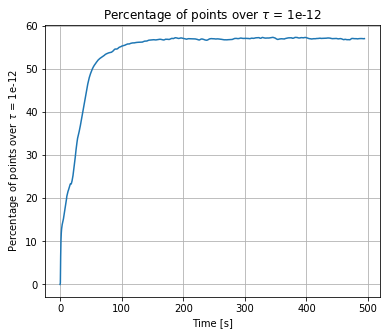
\includegraphics[width = 0.7 \textwidth]{figures/DataAnalysis/SumDataTime}
	\caption{Percentage of significant points in function of the time for $\tau = 10^{-4}$}
	\label{fig:sumtime}
\end{figure}


Furthermore, we decide to \textbf{round to zero} the values that are smaller than the previous threshold of $\tau = 10^{-4}$. This can be motivated by the fact that it will allow to use the sparsity of the data to make the algorithm faster. This means that we will approximatively set a 66\% of the tracer values to zero.\\

We try to find a trend in the data that we could exploit in the rest of the project. We plot for example the mean tracer value for each location in function to the distance to the origin of the tracer. This scatter plot can be seen on figure \ref{fig:tracerdistance}. 

\begin{figure}[]
\centering
	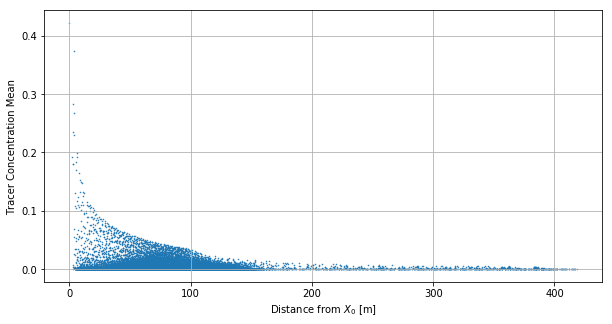
\includegraphics[width = 0.7 \textwidth]{figures/DataAnalysis/TracerMeanDistance}
	\caption{Mean value for each point in function of the distance to the tracer's origin}
	\label{fig:tracerdistance}
\end{figure}


As we can see there is no immediate trend that can be detected, so we proceed to a \textbf{centering of the Data} that will enable a faster processing of the covariance matrix. 



















%%%%%%%%%%% CHAPTER: CONCLUSION
\chapter{Conclusion}

In this report, we have stated some of the research that was done in order to solve the sensor position optimisation problem. \\ 

The biggest challenge here is to make the algorithm scalable for optimising over $100'000$ sensor locations. It requires to develop strategies to make the GPs scalable. The main other challenge is to find a method to accurately estimate the covariance matrix. \\

I have implemented some of the optimisation algorithm proposed on a smaller dataset and with a poor estimation of the covariance function. It has given consistent results and has proven that once the main challenges, described earlier are solved, we will have a good optimisation algorithm for that kind of setups. 



\appendix 

\chapter{Ethical and Professional Considerations}


Throughout this project, I wasn't confronted by any ethical questions and have therefore not checked any item of the ethical consideration list. My project explored the applications of a study proposing an algorithm for near-optimal sensor positioning. Optimising sensor positions is a very broad subject that has applications in most technical fields. I have applied those algorithms in an environmental context. By placing a reduced number of points optimally, we can help to improve the results of the simulations on pollution concentrations. We can also consider that such application can help to increase the number of similar studies by reducing the cost of actual sensor deployment. Our project can, therefore, be considered as respecting the ethical and professional considerations requirements. 

  



\chapter{Description of the Code}





%%%%%%%%%%%%%%%%%%%%%%%%%%%%%%%%%%%%
%\chapter{Further Developements}


%% bibliography
\bibliographystyle{apa}
\bibliography{bibliography}

\end{document}
